%%%%%%%%%%%%%%%%%%%%%%%%%%%%%%%%%%%%%%%%%%%%%%%%%%%%%%%%%%%%%%%%%%%%%%%%%%%%
%% Author template for Management Science (mnsc) for articles with no e-companion (EC)
%% Mirko Janc, Ph.D., INFORMS, mirko.janc@informs.org
%% ver. 0.95, December 2010
%%%%%%%%%%%%%%%%%%%%%%%%%%%%%%%%%%%%%%%%%%%%%%%%%%%%%%%%%%%%%%%%%%%%%%%%%%%%
\documentclass[mnsc,blindrev]{informs3}
%\documentclass[mnsc,nonblindrev]{informs3} % current default for manuscript submission

% \OneAndAHalfSpacedXI
%%\OneAndAHalfSpacedXII % Current default line spacing
%%\DoubleSpacedXII
\DoubleSpacedXI

% If hyperref is used, dvi-to-ps driver of choice must be declared as
%   an additional option to the \documentclass. For example
%\documentclass[dvips,mnsc]{informs3}      % if dvips is used
%\documentclass[dvipsone,mnsc]{informs3}   % if dvipsone is used, etc.

% Private macros here (check that there is no clash with the style)

%https://tex.stackexchange.com/questions/400692/different-height-of-tikz-subfigures-despite-same-axis-width-height
\usepackage{lscape}
\usepackage{booktabs}
\usepackage{array}%[=2016-10-06]
%\usepackage{tabu}
\usepackage{tabularray}
\usepackage{colortbl}

\newcolumntype{P}[1]{>{\centering\arraybackslash}m{#1}}
\usepackage{multirow,calc,amsmath}
\newlength\mylenA
\newlength\mylenB
\newlength\mylenC
\newlength\mylenD
\usepackage{tikz}
\usepackage{tcolorbox}
\usepackage{etoolbox}
%\documentclass{article}
\usepackage{booktabs}
\usepackage{siunitx}
\AtBeginEnvironment{tcolorbox}{\normalsize}

\usepackage{multirow}
\usepackage{placeins}
\usepackage{tabularx}
\usepackage{float}
\usepackage{pdflscape}
\usepackage{amssymb}
\usepackage{algorithm} 
\usepackage{algorithmicx}
\usepackage{algpseudocode}


\usepackage{adjustbox}[valign=t]

\tcbuselibrary{skins, breakable}

\makeatletter
\tcbset{
  tabular/.style={
    boxsep=\z@,top=\z@,bottom=\z@,leftupper=\z@,rightupper=\z@,
    toptitle=1mm,bottomtitle=1mm,boxrule=0.5mm,
    fontupper=\small,
    before upper={\arrayrulecolor{tcbcolframe}\def\arraystretch{1.1}%
      \tcb@hack@currenvir\tabular{#1}},
    after upper=\endtabular\arrayrulecolor{black}},
}
\makeatother

\makeatletter
\patchcmd{\ALG@step}{\addtocounter{ALG@line}{1}}{\refstepcounter{ALG@line}}{}{}
\makeatother

\usepackage{color, colortbl}
\usepackage{graphicx}
%\usepackage{subfigure}
\usepackage{caption}
\usepackage{subcaption}
%\usepackage{tcolorbox}

\usepackage{amsmath}
%\usepackage{amsthm}
\usepackage{dsfont}
%\usepackage{statmath}
\usepackage{mathtools}
\usepackage{physics}
\usepackage{xcolor}
\usepackage{hyperref}
\usepackage{makecell}
% \usepackage{pgfplots}
% \usepackage{tikzviolinplots}
% \usepgfplotslibrary{external}
% \tikzexternalize
% \usepackage{minted}
% \usemintedstyle{gruvbox-light}
% \usepackage{scontents}


 
% \newtheorem{theorem}{Theorem}[section]
% \newtheorem*{theorem*}{Theorem}[section]
% \newtheorem{corollary}{Corollary}[theorem]
% \newtheorem{lemma}[theorem]{Lemma}
% \newtheorem{proposition}[theorem]{Proposition}
% \newtheorem{remark}[theorem]{Remark}
% \newtheorem*{remark*}[theorem]{Remark}

\newcommand{\bx}{\mathbf{x}}
\newcommand{\bu}{\mathbf{u}}
\newcommand{\by}{\mathbf{y}}
\newcommand{\bA}{\mathbf{A}}
\newcommand{\bB}{\mathbf{B}}
\newcommand{\bX}{\mathbf{X}}
\newcommand{\bY}{\mathbf{Y}}
\newcommand{\bZ}{\mathbf{Z}}
\newcommand{\bI}{\mathbf{I}}
\newcommand{\bH}{\mathbf{H}}
\newcommand{\bW}{\mathbf{W}}
\newcommand{\bxi}{\boldsymbol{\xi}}
\newcommand{\bXi}{\boldsymbol{\Xi}}
\newcommand{\bS}{\boldsymbol{\Sigma}}
\newcommand{\bG}{\boldsymbol{\Gamma}}
\newcommand{\mD}{\mathcal{D}}
\newcommand{\mG}{\mathcal{G}}
\newcommand{\mM}{\mathcal{M}}
\newcommand{\mE}{\mathcal{E}}
\newcommand{\gray}{\rowcolor[gray]{.90}}
% Natbib setup for author-year style
\usepackage{natbib}
 \bibpunct[, ]{(}{)}{,}{a}{}{,}%
 \def\bibfont{\small}%
 \def\bibsep{\smallskipamount}%
 \def\bibhang{24pt}%
 \def\newblock{\ }%
 \def\BIBand{and}%
\def\pipeline{Explanation Pipeline}
\newcommand{\tw}[1]{\textcolor{black}{Tong: #1}}

\def\checkmark{\tikz\fill[scale=0.4](0,.35) -- (.25,0) -- (1,.7) -- (.25,.15) -- cycle;} 

% \newtheorem{theorem}{Theorem}
% \newtheorem{corollary}{Corollary}[theorem]
% \newtheorem{lemma}[theorem]{Lemma}
\newtheorem{thm}{Theorem}
\newtheorem{remark2}[thm]{Remark}
%\newtheorem{proof}{Proof}


%% Setup of theorem styles. Outcomment only one.
%% Preferred default is the first option.
\TheoremsNumberedThrough     % Preferred (Theorem 1, Lemma 1, Theorem 2)
%\TheoremsNumberedByChapter  % (Theorem 1.1, Lema 1.1, Theorem 1.2)
\ECRepeatTheorems

%% Setup of the equation numbering system. Outcomment only one.
%% Preferred default is the first option.
\EquationsNumberedThrough    % Default: (1), (2), ...
%\EquationsNumberedBySection % (1.1), (1.2), ...

% For new submissions, leave this number blank.
% For revisions, input the manuscript number assigned by the on-line
% system along with a suffix ".Rx" where x is the revision number.
\MANUSCRIPTNO{MS-0001-1922.65}

%%%%%%%%%%%%%%%%
\begin{document}
%%%%%%%%%%%%%%%%

% Outcomment only when entries are known. Otherwise leave as is and
%   default values will be used.
%\setcounter{page}{1}
%\VOLUME{00}%
%\NO{0}%
%\MONTH{Xxxxx}% (month or a similar seasonal id)
%\YEAR{0000}% e.g., 2005
%\FIRSTPAGE{000}%
%\LASTPAGE{000}%
%\SHORTYEAR{00}% shortened year (two-digit)
%\ISSUE{0000} %
%\LONGFIRSTPAGE{0001} %
%\DOI{10.1287/xxxx.0000.0000}%

% Author's names for the running heads
% Sample depending on the number of authors;
% \RUNAUTHOR{Jones}
% \RUNAUTHOR{Jones and Wilson}
% \RUNAUTHOR{Jones, Miller, and Wilson}
% \RUNAUTHOR{Jones et al.} % for four or more authors
% Enter authors following the given pattern:
%\RUNAUTHOR{}

% Title or shortened title suitable for running heads. Sample:
% \RUNTITLE{Bundling Information Goods of Decreasing Value}
% Enter the (shortened) title:
\RUNTITLE{The Risk of Extrapolation of Post hoc Explanations}

% Full title. Sample:
% \TITLE{Bundling Information Goods of Decreasing Value}
% Enter the full title:
%change title!!!
\TITLE{From Model Explanation to Data Misinterpretation: Uncovering the Pitfalls of Misusing Post Hoc Explainers for Machine Learning Models in Business Research}
\TITLE{The Curse of Rashomon Effects - From Model Explanation to Data Misinterpretation}
% \TITLE{The Risk of Inferring Data Insights from Post hoc Explanations of Machine Learning Models}

% Block of authors and their affiliations starts here:
% NOTE: Authors with same affiliation, if the order of authors allows,
%   should be entered in ONE field, separated by a comma.
%   \EMAIL field can be repeated if more than one author
\ARTICLEAUTHORS{%
\AUTHOR{Snidely Slippery}
\AFF{Department of Bread Spread Engineering, Dairy University, Cowtown, IL 60208, \EMAIL{slippery@dairy.edu}} %, \URL{}}
\AUTHOR{Marg Arinella}
\AFF{Institute for Food Adulteration, University of Food Plains, Food Plains, MN 55599, \EMAIL{m.arinella@adult.ufp.edu}}
% Enter all authors
} % end of the block

% palette for colorblindness https://davidmathlogic.com/colorblind/#%23000000-%23E69F00-%2356B4E9-%23009E73-%23F0E442-%230072B2-%23D55E00-%23CC79A7

\ABSTRACT{%
Machine learning models have been increasingly used in business research. However, most state-of-the-art machine learning models, such as deep neural networks and XGBoost, are black boxes in nature. Therefore, post hoc explainers that provide explanations for machine learning models by, for example, estimating numerical importance of the input features, have been gaining wide usage. Despite the intended use of post hoc explainers being explaining machine learning \textit{models}, we found a growing trend in business research where post hoc explanations are used to draw inferences about the \textit{data}. In this work, we investigate the validity of such use. Specifically, we investigate with extensive experiments \emph{whether} the explanations obtained by the two most popular post hoc explainers, SHAP and LIME, provide correct information about the true marginal effects of $X$ on $Y$ in the data, which we call data-alignment. We then identify \emph{what} factors influence the alignment of explanations. Finally, we propose a set of sensitivity analyses to improve the data-alignment of explanations and demonstrate their effectiveness with real-world data in an econometric context. In spite of this effort, we nevertheless conclude that it is often not appropriate to infer data insights from  post hoc explanations. We articulate appropriate alternative uses, the most important of which is to facilitate the proposition and subsequent empirical investigation of hypotheses. The ultimate goal of this paper is to caution business researchers \textit{against} translating post hoc explanations of machine learning \textit{models} into potentially false insights and understanding of \textit{data}.
%\textcolor{black}{add somewhere that we prove theoretical evidence that SHAP is unsuited for this task}
}%

% Sample
%\KEYWORDS{deterministic inventory theory; infinite linear programming duality;
%  existence of optimal policies; semi-Markov decision process; cyclic schedule}

% Fill in data. If unknown, outcomment the field
\KEYWORDS{post hoc explanation, explainable machine learning, XAI, interpretable machine learning} %\HISTORY{This paper was first submitted on April 12, 1922 and has been with the authors for 83 years for 65 revisions.}

\maketitle

% use statistics of the citation of the post hoc papers
% show how difficult it is to solve the problem, e.g., cite cynthia's paper
\section{Introduction}
    % Mention Marketing Science Institute "consistently identified attribution as a topmost research priority over the last few years" (from SHAP meets uniform paper)

% =========================== Tong ===========================
Over the past few decades, the surge in data volume and complexity has led to the widespread adoption of machine learning (ML) for business analysis \citep{kleinberg2015prediction,mullainathan17applied}. ML is commonly used in scenarios where researchers focus on predicting a particular variable of interest. This translates into formulating a supervised learning problem where the target variable is predicted by an ML model using explanatory variables (features) as inputs.

However, in business research, prediction alone is often insufficient. Researchers and practitioners are also interested in gaining insights about their data through ML models. In particular, they seek information about how explanatory variables are associated with the target variable, measured by some definition of feature importance. %\textcolor{black}{Such information is generally referred to as \emph{feature importance}}. %a relationship that can be described by the marginal effects of the explanatory variables.\footnote{Note that marginal effects are descriptive and do not directly indicate causality unless certain key assumptions, such as exogeneity, no omitted variable bias, etc., hold.} 
%\textcolor{black}{Feature importance can be formulated mathematically in various ways, but the phrase \emph{feature importance} is often undefined when used in research papers, with authors relying on researchers' common understanding of feature importance as a vague, prescientific concept.} \textcolor{black}{Given the lexical ambiguity of the term \emph{feature importance}, this paper undertakes the important and novel task of investigating SHAP and LIME's abilities to extract information in terms of different, common types of feature importance.}
Unfortunately, most ML models with high accuracy operate as black boxes\footnote{It is worth acknowledging that recent years have seen the emergence of inherently interpretable models that can attain comparable performance to black box models, sans the reliance on post hoc explanations. However, these models, which lie beyond the purview of this paper's discussion, will not be further delved into here.} that produce predictions without providing any information about the explanatory variables. Thus, researchers often cannot obtain data insights directly from their predictive models.


In response to the opacity of black box models, post hoc explainers have naturally garnered significant attention from business researchers. Explainers provide various types of explanations of black box models, such as feature importance \citep{ribeiro16lime,lundberg17shap}, partial dependence plots \citep{friedman01pdp}, counterfactual examples \citep{mothilal20dice}, etc. Many recent works in business research follow a two-stage pipeline that we will call the \emph{Explanation Pipeline}. The Explanation Pipeline, which is illustrated in Figure \ref{fig:pipeline}, consists of a first stage where a black box ML model is employed for a prediction task, and a second stage where the ML model is explained by a post hoc explainer. This pipeline enables researchers to gain some understanding of the model's decision-making process, such as the importance of different features.% \textcolor{black}{in terms of Shapley values}. % feature importance for the ML model,  from which they draw some conclusions on the features as if they are using $\boldsymbol{\beta}$s.

% \textcolor{black}{In this paper we will expose factors present in each stage of the explanation pipeline (model generation and explanation generation) that hamper attempts at understanding data through ML models.}

% \textcolor{black}{One very important factor in the fist stage, called the Rashomon effect, is a relatively new idea in ML that has been very impactful in XAI in recent years. Simply put, the Rashomon effect means that given a dataset we can train many models that are equally good at prediction, yet each represent a different hypothesis about how the input features determine the output. As a result, we cannot necessarily trust that a model's good predictive performance is indicative that the input features are important to the model in all of the same ways that the input features are important in the ground truth data generation process. Furthermore, we will also show that different properties of data, such as the presence of correlated or confounded features, are also problematic. These properties of the data are associated with undesirable properties of ML models that can manifest in different ways across the Rashomon set.} 


% \textcolor{black}{Since, given an input dataset, factors in stage 1 place a limit on how faithfully an ML trained on that dataset can represent the ground truth DGP, it is important to ask: \emph{Can we use post hoc explainers in stage 2 to extract the kernel of truth a model possesses about the DGP?}} 
Although post hoc explanations are intended to explain ML models, a growing number of research papers seem to rely on the expectation that such explanations can be extrapolated to understand the \textbf{data} rather than the model. This expectation is particularly pertinent for explainers that produce feature importance, such as Local Interpretable Model-Agnostic Explanations (LIME) \citep{ribeiro16lime} and Shapley Additive Explanations (SHAP) \citep{lundberg17shap}.
Indeed, recent literature increasingly adopts this problematic perspective. SHAP and LIME explanations of black box models have been extrapolated in diverse areas of business literature to make inferences about the marginal effects of the features. For instance, \cite{park2024extracting} claims that SHAP explanations provide guidance on what smartphone features customers prefer. \cite{jiang24churn} says that if a customer has a large value for a feature with large SHAP values, they are more likely to be churners, and \cite{sanchez2023role} claims that their SHAP explanations reveal what factors actually drive hotel guest satisfaction and and so hotel managers should plan their service strategies accordingly. Some recent work is quite optimistic about post hoc explanations - \cite{berger2023supply} advocates the use of the combination of an ML model and SHAP as an ``alternative to OLS."

\textcolor{black}{we may need to update this paragraph to reflect recent survey}
To gain a deeper understanding of the prevalent practice of employing post hoc explanations in business research, we conducted a thorough review of the literature. Specifically, we surveyed more than 700 papers from the business literature published between 2018 and 2024 \textcolor{black}{do we survey till 2024 or 2025?}  that cited SHAP or LIME\footnote{LIME was published in 2016, and SHAP was published in 2017. Considering the time it takes to write a business paper, we set the start time of our literature search to 2018 for papers that use either LIME or SHAP.}  and manually identify 150 that actually used SHAP or LIME to obtain post hoc explanations. 109 of them have been published in top journals.\footnote{We consider a journal a top journal if the 5-year impact factor is above 5 or the journal is an INFORMS journal. Note that SHAP and LIME are relatively new methods, and the business journal review processes are long. Therefore, many of the remaining papers are still under review and are not counted among the 109 top journal papers we reviewed.} The remaining 41 papers include papers from SSRN that have yet to complete the long review process of business journals. We have meticulously analyzed these 150 papers and found that among them, 42\% used the post hoc explanations to draw inferences about the \textit{data}, rather than the ML \textit{model} being explained. Their conclusions and putative insights can be roughly categorized into \textcolor{black}{uses of four} dominant types \textcolor{black}{of feature importance}. 

\textcolor{black}{These first three} claims aim to describe or partially describe the marginal effect of $X$ on $Y$ in the data. 
First, papers make claims about the qualitative relationships between $X$ and $Y$, most commonly about whether an $X$ has a positive or negative relationship with $Y$. They use language like ``$X_j$ has a positive/negative impact on $Y$,'' when the explainer provides a positive/negative feature importance for feature $X_j$. Second, papers infer the relative importance of the features from post hoc explanations. They use language like ``$X_1$ is more important to $Y$ than $X_2$ is" if the feature importance of $X_1$ is larger than that of $X_2$. Third, some papers would use post hoc explanations to identify the most influential features and use language like ``$X_{j_1}, X_{j_2}$, and $X_{j_3}$ are the most important to $Y$" when the feature importance for $X_{j_1}, X_{j_2}$, and $X_{j_3}$ are greater in magnitude than the others. Such use of explainers suggests an emerging paradigm shift in which, through post hoc explanations, ML models are used not only for prediction but also to gain understanding of data. However, the validity of using explainers for this purpose remains unjustified. 

\textcolor{black}{In addition to interpreting \emph{feature importance} in terms of marginal effects, researchers also interpret/understand the importance of a feature in terms of how it affects different outcomes related to ML models. Specifically, a feature can be viewed as important because predictive performance seems to be sensitive to the inclusion of that feature. This is the fourth type of claim. The fifth and final type of claim occurs when research assert that a feature is important because varying it allows them to construct counterfactual instances.}


  % \citep{lorentzen2020peeking}. 
      \begin{figure}[t]
        \centering
        %\fbox{
\includegraphics[width = \textwidth,trim=250 500 150 250 mm, clip=true]{Figures/pipeline.pdf}}
        
\includegraphics[trim={4.75cm 7.5cm 1.125cm 4.25cm},clip, width = 0.9\textwidth]{Figures/pipeline_flow_new.pdf}
        \caption{Explanation Pipeline: the pipeline of using post hoc explainers to explain a machine learning model. Additionally inferring information about the actual marginal effects of the features constitutes mistaken usage of the pipeline.}
        \label{fig:pipeline}
    \end{figure}
     % They build a black box ML model for a complicated task, which could have many variables, or strong interactions of variables, or include unstructured data, such that canonical econometric methods do not easily apply. Then a post hoc explainer is used to generate feature importance for the ML model,  from which they draw some conclusions on the features as if they are using $\boldsymbol{\beta}$s. 
 

 
 % In addition, there are many types of feature importance \citep{AchenChristopherH1982Iaur}. However, except for \citep{lorentzen2020peeking}, the works cited in the previous paragraph did not provide a formal definition of feature importance and justify that the explainer(s) used were actually providing that type of feature importance. Similarly, the basic question of why Shapley values are appropriate feature importance measures is never addressed in these works\footnote{It is argued in \citep{kumar20shap} that Shapley values are not conducive to human understanding of feature importance.}. 


%Therefore, the goal of this paper is to urge the research community to approach post hoc explanations with skepticism and a more critical eye. 
% We argue in this paper that there exist fundamental flaws in using post hoc explanations to elicit information on $\boldsymbol{\beta}$s. 
Therefore, the goal of this paper is to conduct a thorough investigation into this new and emerging trend of research methodology. We aim to directly answer the question, 
``\emph{Can SHAP and LIME explanations \textcolor{black}{correctly characterize the relationship between $X$ and $Y$ in the data in terms of different popular notions of feature importance?}}''
with both empirical and theoretical evidence.  

\textcolor{black}{To begin, we investigate whether the SHAP and LIME explanations align with the true marginal effects using simulated data from a simulated linear ground truth model. We do this because in such cases the ground truth marginal effects are easy to derive and understand.} For this purpose, we design three \textit{new} metrics that assess post hoc explanations in terms of capturing correct information about the true marginal effects. %The first metric evaluates whether an explanation's feature importance values have the same signs as the corresponding marginal effects. We call it the \textbf{directionality} of an explanation, since it represents how well an explanation identifies the directions in which features influence the target. The second metric evaluates how much the ranking of features by a post hoc explanation agrees with the ranking induced by the marginal effects. We call it the \textbf{concordance} of an explanation. The last metric evaluates whether a post hoc explanation identifies the most important features. We call it the \textbf{relevance} of the explanation.
These metrics assess the extent to which the explanations are consistent with the marginal effects in terms of the sign, the ranking of features, and the identification of the most important features. %We call the evaluation of these three metrics the test of \textbf{data-alignment}.
%We evaluate the data-alignment of post hoc explanations using simulated data where we know and can control the ground truth marginal effects in the data. We set our ground truth models to be linear because the extent an explainer can produce data-aligned explanations of simple linear models is  indicative of its potential for data-alignment in more general scenarios -- if an explainer cannot give data-aligned explanations of simple linear phenomena, it is very likely unable to be able to explain the complex processes underlying practical datasets. 
Unfortunately, our findings reveal that SHAP and LIME explanations typically \textit{do not align} with the marginal effects, not even qualitatively (directionality), and the alignment further drops as the feature dimension increases. This misalignment is evident even in straightforward business scenarios with a linear ground truth model and when the black box model being explained demonstrates high predictive performance on data containing all relevant features to $Y$, all of which are mutually independent. 

\textcolor{black}{We then investigate more general cases where the ground truth may be a nonlinear function and the intended notion of feature importance may not be in terms of marginal effects. Specifically, we consider the possibilities that \emph{feature importance} may be given in terms of 1) global ranking 2) instance-level ranking 3) predictive power 4) usefulness for counterfactual generation. We delve into the causes of this misalignment, discovering that various factors within the explanation pipeline affect the explainers' ability to extract information about each of the four kinds of feature importance.} These include having correlated features in the data, the predictive performance of the black box model, and specific settings of explainer model parameters. %We corroborate the initial presentation of our results by showing that misalignment pervades an additional 100 simulations where we explain models produced using AutoML that were trained on datasets with varying numbers of features, rows, and label noise.

\textcolor{black}{We also offer various theoretical justifications for data misalignment}.
\textcolor{black}{Our central claim is that the \emph{Rashomon effect}, in which there exists a multiplicity of distinct models with equivalent (near-optimal) performance, makes use of the explanation pipeline questionable at the outset.} Additionally, we show that SHAP explanations inherently fail to align with the marginal effects, making Shapley values fundamentally inappropriate for any definite claims regarding marginal effects. We show that SHAP estimates situational importance~\citep{StrumbeljErik2014Epma}, 
 which expresses the consequence of a feature taking on a value different from its mean. Although the computation of situational importance for a feature involves its marginal effect, the information it contributes can be destroyed in the process. Furthermore, we present theoretical grounds for conditions under which LIME might achieve a high degree of data-alignment.

% \textcolor{black}{I think we should say SHAP and LIME separately. }

% We then demonstrate another critical issue of post hoc explanations: inconsistency. Inconsistency refers to the difference in explanations produced by different configurations within the Explanation Pipeline. Using the same simulated data, we show that varying choices along this pipeline can lead to significantly divergent, and occasionally opposing, explanations. It then follows from the view that the purpose of science is to identify phenomena that occur without fail that post hoc explainers have very limited utility to researchers.


Finally, we propose a set of sensitivity analyses for explanations provided by SHAP and LIME. Although our theoretical and empirical findings suggest that it is not possible to fully eliminate the issue of data-misalignment, they nevertheless reveal opportunities for improvement, which we address. For instance, for SHAP, the most immediate way to increase data-alignment is to divide its Shapley values by the differences between the corresponding feature values and their means; for LIME, increasing some hyperparameters will significantly increase the alignment with the data.
Another strategy that showed promise involves averaging the explanations derived from a family of accurate models. We also observe that when the training data used by a black box model include all relevant features, all of which are independent, the alignment of explanations of the black box's predictions with the ground truth tends to increase. This suggests that the underlying data quality and structure play a significant role in the effectiveness of post hoc explanations.
However, other intuitive strategies we tested, such as combining explanations from both SHAP and LIME for a single black box model, did not yield effective results. This highlights the complexity of the issue and the need for more nuanced solutions.
\textcolor{black}{It is also important to note that our sensitivity analyses degrees are limited by XYZ...} Consequently, post hoc explainers should be used with great caution by business researchers, and the appropriate uses of these tools must be clarified.


Overall, our paper identifies and cautions against a growing trend of the inappropriate use of post hoc explanations to draw inferences about data, leading to data misinterpretation. We argue that post hoc explanations should not be used to \textbf{validate} hypotheses about data; instead, their role in gathering knowledge about data should be limited to \textbf{proposal} of hypotheses. To gain an accurate understanding of the underlying relationships  the data, we emphasize the need for more rigorous and comprehensive follow-up analyses, both quantitatively and qualitatively. This distinction is essential to ensure the prevention of the overestimation of the reliability and validity of insights derived from post hoc explainers in business research.


    The paper is organized as follows. We will review related work pertaining to SHAP, LIME, and their weaknesses in Section \ref{sec:related_work}. Section \ref{sec:use_in_b_research} focuses on the use of SHAP and LIME in business literature, showing the prevalence of inappropriate usage. Then we use a simulated dataset with ground-truth models that we created to demonstrate the Explanation Pipeline and its vulnerabilities in Section \ref{sec:pipeline_demo}.  We provide theoretical and empirical analyses on why post hoc explanations are not suitable to infer information about marginal effects in Section \ref{sec:linear_case}. 
    We then showcase some sensitivity analyses for SHAP and LIME in Section \ref{sec:mitigation_strategies} and subsequently gauge how beneficial they are over baselines in reproducing the findings of an econometric study carried out using real loan application data in Section \ref{sec:case_study}. The paper concludes in Section \ref{sec:discussion} with a summary of our findings and final remarks on post hoc explanations and their appropriate use in business research. In the appendix, we provide additional details about our experimental designs and  corroborate results of Section \ref{sec:causes_of_misalignment} by repeating the experiment on another dataset.% \tw{do we have mitigation tested on a new dataset as well? if so we should say it}

    \textcolor{black}{experiments centers around three pillars: i) data; ii) intended estimand; iii) evaluation metric. Need to focus more on population level (aggregated)}
\section{Related Work}
    \label{sec:related_work}
    This section introduces the Rashomon effect, SHAP and LIME, and then reviews the prior literature that discusses their weaknesses from perspectives different from our paper. %Weaknesses discussed include intrinsic (theoretical) issues due to how the explainers are designed, and practical issues users may face due to those intrinsic issues. 

    
    \subsection{Rashomon Sets and The Rashomon Effect}
        \textcolor{black}{Initially given a data-scientific meaning by Leo Breiman, the \emph{Rashomon Effect} in data science refers to the phenomenon in classification where there is a collection of models with roughly equivalent (near-optimal) predictive performance, but each model in the collection has a unique way of using the input features to produce predictions~\cite{donnelly2023rashomon,rudin2024amazingthingscomehaving} As a result, feature importance is different for each model.\footnote{To see the idea, consider for the sake of argument a scenario where an astrologer and a CPA are equally accurate at predicting whether individuals will owe money or receive a refund on their yearly taxes.} Paes et al.~showed that the Rashomon effect always occurs when only finite data is available~\cite{paes23inevitable}. Although  models in a Rashomon set have roughly equivalent performance, they need not agree on individual predictions and so explanations of models on unseen/unlabeled data is even more treacherous~\cite{hsu2022rashomon}. }  

    \subsection{Post Hoc Explainers - SHAP and LIME}
     SHAP \citep{lundberg17shap} and LIME \citep{ribeiro16lime}  are the two most widely used model-agnostic post hoc explainers. %Model agnosticism refers to the ability to explain any ML model without the access to the internals of the ML model, i.e., only using the input and output of a model. Attributive explainers explain the predictions of a predictive ML model by attributing numerical feature importance values to each input feature. Both SHAP and LIME represent feature importance using the coefficients of an additive feature importance model. %Counterfactual explainers such as WachterCF\citep{wachter17wachtercf} and DiCE\citep{mothilal20dice} are of secondary importance and explain an output of an ML model by providing a contrasting input that cause the model to produce a different output. 
        We use SHAP and LIME as representatives for post hoc explainers in this paper because they are also the dominant choices for post hoc explainers in business research.

        % Counterfactual explainers explain an output of an ML model by providing a contrasting input that cause the model to produce a different output. It is desirable for the contrasting input to be as close to the original as possible in order to identify a minimal change that yields a different output. Examples of counterfactual explainers include WachterCF\citep{wachter17wachtercf} and DiCE\citep{mothilal20dice}.
        
     %SHAP and LIME are model-agnostic attributive post hoc explainers. They are model-agnostic in the sense that they can explain any ML model.  Standard implementations of SHAP and LIME can explain both classification and regression models using tabular, text, or image data as input.


SHAP (SHapley Additive exPlanations) is a groundbreaking approach in the field of interpretable machine learning that offers a unified measure of feature importance. Developed by Lundberg and Lee in 2017, it builds on the concepts of game theory, particularly the Shapley value, to assign an importance value to each feature for a particular prediction. The fundamental idea behind SHAP is to assess the contribution of each feature to the difference between the actual prediction and the average prediction over the dataset. One of the unique aspects of SHAP is its consistency and local accuracy. The method guarantees that if a model changes in a way that makes a feature more important, the SHAP value of that feature will not decrease. Local accuracy ensures that the contributions of all features sum up to the actual prediction minus the average prediction, providing a detailed and accurate decomposition of the prediction. Note that LIME does not have this local accuracy property. There are several variants of SHAP, such as Kernel SHAP \citep{lundberg17shap}, TreeSHAP \citep{lundberg2018consistent} and DeepSHAP \citep{lundberg17shap}. Each variant retains the core principles of SHAP while adjusting the computational strategy to suit the specific model architecture, ensuring that the interpretability benefits of SHAP can be realized across a wide range of machine learning models.
    % SHAP's additive feature importance model differs from LIME's in that the coefficient of each feature represent the Shapley value~\citep{shapley97shapley} of that feature. SHAP surrogate models are not fit on sampled training data instances directly like LIME's, but rather on sampled coalition vectors (binary vectors indicating presence of each feature). Shapley values were originally a game-theoretic notion meant to quantify how much each player contributed to the final score of a game. In the context of SHAP, the Shapley values (surrogate model coefficients) represent how much the value of the feature to which they correspond contributes to the final value of the black box model's prediction. 

    
 % Underlying LIME explanations are ridge regressors fitted on data sampled around the input datum being explained. 
Although not used as widely as SHAP in business research, LIME is the very first model-agnostic post hoc explainer. It was developed by \citet{ribeiro16lime}. LIME trains a ridge regressor on a synthetic dataset constructed by sampling uniformly around the input datum. The coefficients of the ridge regressors indicate the importance of each feature. LIME discretizes numerical features into quartiles to avoid dealing with problems associated with differing scales of features and ensure users do not get confused when interpreting negative weights for negative valued features. The ridge regression's optimization weighs the sampled data with an exponential kernel and includes an $L_1$ (LASSO) penalty. LIME uses the $L_1$ regularization so that the regressor it produces is sparse in the sense that, rather than including all features, only a subset of features that are most influential for predictions near the instance being explained are included. This makes LIME's explanations more concise than they would be otherwise. The ridge regressors are called surrogate models because they are trained to approximate the predictions of the black box model.
    
    LIME's ridge coefficients are meant to represent marginal effects, but depending on the LIME variant and the model being explained, they are not the gradient of the black box model at the input being explained. \citet{garreau2020looking} proved that the original LIME formulation's coefficients did not, in general, equal the gradient of the black box model at the input being explained. Instead, each feature importance value is proportional to the partial derivative of the black box at the input datum and the proportionality constants differ by feature. \citet{agarwal21clime} showed that a simpler variant of LIME called C-LIME that does not discretize input features and does not perform weighted ridge regression produced coefficients that are proportional to the gradient of the black box model. %Removing discretization allows C-LIME to recover the gradient because otherwise, local information about the black box's decision boundary is destroyed.
    In discretizing features, the data used in LIME's regression problem consists of binary features indicating which bins (quantiles) the feature values of sampled data fall into, which destroys the gradient since the local information about the black box's decision boundary is lost. Moreover, C-LIME drops the ridge penalty because enforcing sparsity opposes the goal of recovering the gradient. In the specific case where the model being explained is linear, C-LIME recovers the coefficients of the linear model. This being the case, in this paper, we choose to disable the discretization setting of LIME throughout the paper to improve the quality of LIME explanations.



    \subsection{The Evaluation of Post hoc Explanations}
        \label{sec:cs_critique}
        The alarm for post hoc explanations had first gone off in the field of machine learning, as researchers questioned the correctness and validity of post hoc explanations. However, the notions of correctness and validity in the ML literature differ from the point of view we take in this paper. The ML community's attention has mainly focused on explanation quality \textbf{with respect to the ML model} since the primary goal of the machine learning field is to develop new models that make better or faster predictions. In addition, they consider factors relating the ability of humans to interpret the explanations, most of which do not fall within the scope of our critique. Thus, the way the ML community evaluates explainers is different from how we evaluate them in this paper.

    
        That post hoc explainers misrepresent the black boxes they explain is a pillar of the ML community's critique. The terms \emph{fidelity} and \emph{faithfulness} are used interchangeably and generally represent the maxims of completeness and soundness outlined by \cite{zhou21evaluating}. An explanation is complete if it is a full characterization of the black box's behavior. An explanation is sound if its characterization is correct.\footnote{In this paper, however, we characterize faithfulness in reference to the ground truth instead of the black box model because we are interested in obtaining insights about reality, not about black box models. In Section \ref{sec:evaluating_faithfulness}, we define metrics that capture our notion of faithfulness.} 
    \cite{garreau2020looking} and \cite{han22which} consider soundness from a function approximation perspective, directly measuring the difference between an explainer  and the black box model. \cite{garreau2020looking} shows that LIME's approximation error is always bounded away from 0. \cite{han22which} analyzes kernelSHAP and LIME relying on a view of KernelSHAP and LIME as kernel weighted linear regression models whose input data are sampled by perturbing the input by random noise. They remark that the choice of noise distribution made by kernelSHAP and LIME prevents them from being able to recover the gradient of linear models they explain as feature importance values. It follows that KernelSHAP and LIME cannot necessarily be expected to reliably perform their intended task of interpreting black box model behaviors. 
Other fidelity/faithfulness metrics measure particular approximation properties such as the extent to which an explainer assigns zero importance to features the model does not depend on are used as metrics in \cite{nguyen2020quantitative}. Metrics such as Deletion and Insertion metrics are based on the idea that features said to be important by an explainer should have significant effects on black box output \citep{deyoung20eraser,nguyen2020quantitative,alvarez18robustness,luss2021leveraging}. \textcolor{black}{And \citet{slack19fooling} demonstrate that post hoc methods like LIME and SHAP are vulnerable to adversarial manipulation, allowing model explanations to be deliberately distorted through targeted attacks.Moreover, \citet{fernandez20explaining} focus on explaining AI decision-making processes, contrasting counterfactual explanations with feature-importance methods like SHAP and LIME, and highlighting conditions under which the former better captures how features influence decisions.} However, all previously mentioned papers study the fidelity with respect to the \textit{ML model}, rather than the data, as we do in this paper. Nevertheless, the aforementioned studies partially answer our research question -- if a black box explainer has difficulty even being faithful to an ML model, it would be even more challenging for it to provide correct data insights.
%The underlying supposition of Deletion and Insertion metrics is that removing or adding features said to be important to a prediction by an explainer should change the prediction to change substantially \citep{deyoung20eraser,nguyen2020quantitative,alvarez18robustness,luss2021leveraging}. %Some works evaluate explainers by taking advantage of contexts where feature importance information of a model is known. \cite{blunsom2019can} evaluates explainers of a white box recurrent model by quantifying the explainers' error rates with respect to identifying important tokens in inputs. \cite{carmichael21framework} evaluates additive explainers by calculating the Jaccard index between the sets of effects present in neural networks and GAMs and the effects and associated contributions of features given by explainers for those models. 
    
  The ML community has also largely focused on other aspects of post hoc explanations, such as interpretability or understandability of the explanations. Explainers which satisfy desiderata related to interpretability should be able to provide a description of the behavior of a black box model in a form which can be easily understood by humans. For example, explanations should be simple enough to be intelligible but complex enough so that the explanation is still complete and sound. Parsimony \citep{nguyen2020quantitative} and clarity \citep{lakkaraju2017interpretable,montavon2018methods,alvarez18robustness} metrics, for example, measure the simplicity and ambiguity of explanations, respectively\footnote{We use the terminology of \cite{markus2021role} here.}. \cite{jacovi2023diagnosing} further requires that the form of explanations match what the psychology literature identifies as natural for human understanding.  Simplicity of explanations beyond the per-feature importance values given by attributive explainers is not desirable in our application because, e.g. artificial enforcement of sparsity could encourage explanations to omit information about the marginal effects and become incomplete and unsound as a result. %For example, LIME's use of a LASSO penalty to make its explanations sparse is undesirable because it could cause a feature to have zero importance when the $\beta_j$ for that feature is non-zero. %Futhermore, stability metrics quantify how different explanations of nearby inputs are. The size of the local Lipschitz constant of the function underlying the explainer is one such example \citep{alvarez18robustness}. Stable explanations can be desirable because an explainer's explanations for two similar inputs being very dissimilar could engender mistrust of the explainer or arouse unwarranted suspicion of unfairness in the underlying decision process. These factors, however, are not within the scope of our discussion.

    
   
    
    
    \section{Use of SHAP and LIME in Business Research}
        \label{sec:use_in_b_research}
% \textcolor{black}{This needs to be strengthened, some tables might be helpful. 

% The goal here is to prove that 1) it is a prevalent problem; 2) Even top journals have papers that make this mistake

% => show both the breadth (in terms of the number of papers, number of journals, number of fields within business research), depth (the number of top journals）

% }
% \textcolor{black}{find papers that use post hoc explanation to get insights that resemble $\boldsymbol{\beta}$ (explaining G). Also mention that some papers only use post hoc explainer on M. It is the intended use of the post hoc explanations, but even that faces severe criticism from the ML community discusses explanations for M}

% \textcolor{black}{Move the appendix here}

\textcolor{black}{A small but growing body of research has begun to question the reliability of post hoc explanation methods such as LIME and SHAP. Among them, \citep{slack19fooling} highlight their vulnerability to adversarial manipulation, showing that model explanations can be deliberately distorted through attacks. However, such work typically assumes that explanations are valid under normal conditions. In contrast, our study investigates how these explainers are used in business research even in non-adversarial settings. We argue that many papers misinterpret model explanations as insights about the underlying data-generating process—such as marginal effects or causal relationships—thus misapplying SHAP and LIME beyond their intended scope.}

As part of our literature review process, we cataloged papers at the intersection of business and explainable machine learning. We used Web of Science as the primary source to search for publications citing at least one of LIME \citep{ribeiro16lime} or SHAP \citep{lundberg17shap}, and containing either “LIME” or “SHAP” in the body of the paper. The results were filtered by topics relevant to business, including management, economics, supply chain \& logistics, and operations research \& management science. More than 700 papers were identified.

\begin{figure}[ht]
\centering

\includegraphics[width=.5\textwidth]{Figures/citation_count_new.pdf}
\caption{Year-by-year breakdown of number of papers citing either LIME or SHAP that belong to business-adjacent Web of Science categories.}
\label{apx_tab:citation_count_graph}
\end{figure}

We then iterated through the resulting papers one by one, collecting those that actually used SHAP or LIME to explain machine learning models (many papers only mentioned them in the context of related or future work), until we compiled a set of 150 distinct papers. Among these, 91\% used SHAP and 14\% used LIME to generate explanations, with 5\% using both.

We closely examined these 150 papers and categorized their use of post hoc explanations through a systematic procedure. First, we assessed whether authors correctly understood that SHAP and LIME are intended to explain model behavior, not the underlying data. For those that failed this criterion, we recorded problematic language indicative of misinterpretation and compiled direct quotations. Not all papers exhibited such issues; some clearly restricted the use of SHAP and LIME to model-level explanations.

Based on this assessment, we classified papers into three categories: (1) controversial papers that clearly extrapolated explanations to draw inferences about marginal effects; (2) ambiguous papers with language that could imply such extrapolation; and (3) proper papers that correctly limited explanation to the model outputs.

Our findings indicate that 42\% of the papers were controversial, clearly misusing explanations to infer data-level relationships. An additional 15\% of papers fell into the ambiguous category. Together, over half of the reviewed papers exhibited problematic language. Furthermore, 76\% of the controversial papers appeared in top-tier journals, highlighting a growing trend of misinterpretation in high-impact research.

\textcolor{black}{
While our Web of Science review captures a broad cross-section of the literature, we further sought to assess whether this pattern of misuse extends to the most influential academic outlets. To this end, we conducted a targeted review of top-tier journals in business and management. Specifically, we identified three prominent groups of business-related journals: the UTD 24, the FT50, and journals published by the INFORMS society. While these journal groups overlap, our statistics treat each group independently, meaning journals appearing in multiple lists are counted in each relevant category.}

\textcolor{black}{Using the search functionalities on each journal’s official website, we identified all articles published from 2017 onward that contained the keywords “LIME” or “SHAP”. This process initially produced more than 800 results, from which we manually selected 74 papers that made substantive use of these explainers to interpret machine learning models. As shown in Table \ref{tab:literature_review}, these papers were distributed across the three journal groups, with SHAP being adopted much more frequently than LIME. Importantly, the table also indicates that a substantial proportion of these papers involved controversial usage, underscoring that such practices are not confined to a handful of outlets but appear consistently across leading journals.}

% \begin{figure}[htbp]
%     \centering
%     \begin{subfigure}[b]{0.48\textwidth}
%         
\includegraphics[width=\textwidth]{Figures/journal_group_dis_1.png}
%         \caption{Number of papers using LIME or SHAP in each journal group.}
%         \label{fig:dist_1}
%     \end{subfigure}
%     \hfill
%     \begin{subfigure}[b]{0.48\textwidth}
%         
\includegraphics[width=\textwidth]{Figures/journal_group_dis_2.png}
%         \caption{Number of distinct journals using LIME or SHAP in each journal group.}
%         \label{fig:dist_2}
%     \end{subfigure}
%     \caption{Distribution of SHAP/LIME Papers and Journals Across Top Journal Groups \hl{maybe we should use tables rather than figures. too many figures in this section. combine with table 2}}
%     \label{fig:combined_dist}
% \end{figure}

% \begin{figure}[ht]
% \centering
% 
\includegraphics[width=.8\textwidth]{Figures/field_dist.png}
% \caption{Field distribution of the top journal papers.}
% \label{fig:field_dist}
% \end{figure}

\textcolor{black}{To evaluate the extent of such controversial usage, we classified each paper following the same criteria applied earlier in our Web of Science review, namely whether SHAP or LIME was interpreted as evidence about the data-generating process or used to justify causal claims. Based on this classification, the statistics in Table \ref{tab:literature_review} reveal two key patterns. From the perspective of \textit{papers}, on average more than 40\% of the reviewed articles across the three journal groups engaged in controversial use of post hoc explainers. From the perspective of \textit{journals}, on average more than 60\% of the outlets represented in each group had published at least one paper with controversial usage. Together, these results provide strong evidence that the inferential misuse of SHAP and LIME is not only common across business research but also persistent even in the most reputable academic venues. 
}

\textcolor{black}{We developed a taxonomy of explanation usage to support this classification, which distinguishes categories such as Directionality, Concordance, Explaining Data, and Causality Claims, among others. For transparency, the complete taxonomy along with representative quotations is provided in Appendix E (Table \ref{tab:explanation_categories}). Figure \ref{fig:category_dist} further illustrates the distribution of papers across these categories. As shown in the figure, while the majority of papers employed post hoc explainers to interpret model behavior or to characterize the directionality and concordance of feature importance, a non-negligible fraction of papers used these methods to make claims about the data-generating process or to support broader causal interpretations. This pattern underscores that the most problematic uses, though not dominant, are still sufficiently frequent to warrant concern.}

\begin{table}[htbp]
\centering
\caption{Statistical Summary of LIME and SHAP Usage in 74 Reviewed Papers Across Journal Sets}
\label{tab:literature_review}
\begin{tabular}{lccc}
\toprule
\textbf{Journal Sets} & \textbf{UTD24} & \textbf{FT50} & \textbf{INFORMS} \\
\midrule
\multicolumn{4}{l}{\textbf{Paper Statistics}} \\
\quad Total Papers Reviewed & 57 & 65 & 38 \\
\quad Papers Using LIME & 12 & 15 & 11 \\
\quad Papers Using SHAP & 48 & 54 & 32 \\
\quad Papers with Controversial Use of LIME & 2 & 2 & 1 \\
\quad Papers with Controversial Use of SHAP & 24 & 24 & 14 \\
\quad Papers with Any Controversial Usage & 26 & 26 & 15 \\
\quad Controversial Usage (\%) & 45.6\% & 40.0\% & 39.5\% \\
\midrule
\multicolumn{4}{l}{\textbf{Journal Statistics}} \\
\quad Journals Represented in Review & 17 & 25 & 10 \\
\quad Journals with LIME Use & 8 & 11 & 7 \\
\quad Journals with SHAP Use & 15 & 22 & 8 \\
\quad Journals with Controversial Usage & 14 & 14 & 6 \\
\quad Controversial Usage (\%) & 82.4\% & 56.0\% & 60.0\% \\
\bottomrule
\end{tabular}

\smallskip
\footnotesize
Note: Statistical summary based on a comprehensive review of 76 papers across three journal sets. 
"Journals Represented in Review" indicates the number of distinct journals from each set that were included in the review.
\end{table}

\begin{figure}[ht]
\centering

\includegraphics[width=.8\textwidth]{Figures/category_dist.png}
\caption{Distribution of the top journal papers across use categories.}
\label{fig:category_dist}
\end{figure}

\textcolor{black}{These findings reinforce our central argument: the inferential misuse of post hoc explainers such as SHAP and LIME is not only prevalent across a wide range of business research, but also persistent even in the most reputable academic venues. By combining a large-scale Web of Science review with a focused analysis of top-tier journals, we offer robust evidence that such misinterpretations represent a widespread methodological concern in the field.}

Building on these findings, we further examine how SHAP and LIME are used in the controversial papers identified above. Specifically, we observe that their interpretations of feature importance values often fall into two categories: (1) identifying the directionality of each feature’s impact (i.e., the sign of importance), and (2) ranking features by relative importance.% and (3) selecting a subset of the most important features. 
Table 2 presents representative quotations illustrating these three usage patterns. In Section 6.1, we introduce quantitative metrics to assess the degree to which explainers can reliably support these interpretive tasks. We refer to these metrics as directionality and concordance, respectively.




%         As part of our literature review process, we cataloged papers at the intersection of business and explainable machine learning.
        
%         We searched for papers from three sources. First,  we used Web of Science %and SSRN\footnote{We searched on SSRN because business journal papers usually take a few years to get published so there are many preprints available on SSRN.} 
%         to search for publications citing at least one of LIME~\citep{ribeiro16lime} or SHAP~\citep{lundberg17shap} and have either ``LIME" or ``SHAP" appear in the body of the paper. The results were filtered by topics related to business, such as management, economics, supply chain \& logistics, operations research \& management science, etc. More than 700 papers were identified. See Figure \ref{apx_tab:citation_count_graph} for a breakdown of the number of papers by year.
%                \begin{figure}[ht]
%             \centering
%             
\includegraphics[width=.5\textwidth]{Figures/citation_count_new.pdf}
%             \caption{Year-by-year breakdown of number of papers citing either LIME or SHAP that belong to business-adjacent Web of Science categories.}
%             \label{apx_tab:citation_count_graph}
%         \end{figure} %\tw{I don't like the bar plot. Change the bar plot to gray (black edges and gray fills) }
%         The second source of papers is INFORMS journals. We searched with the same keywords on the INFORMS journal portal. Finally, we searched on SSRN for papers that are not published yet. Because business journal papers usually take a few years to get published, there are many preprints available on SSRN. The total number of papers from these three sources that matched our keywords was over 700. 
        
%         We then iterated through the resulting papers one by one, collecting papers that actually used SHAP or LIME to explain a machine learning model (many papers only mentioned SHAP or LIME in the context of related work or future work) until we had a total of 150 different papers. 
%         Out of these papers, 91\% used SHAP and 14\% used LIME to generate explanations for their models, including 5\% using both of them.


        
%         We took a close look at these papers and characterized their use of post hoc explanations by the following procedure. We first searched for evidence that it was understood that the intended use of SHAP and LIME is to explain model outputs (rather than the data). On those that fail this screening, we identified problematic language indicative of inappropriate use of post hoc explanations and recorded quotations of problematic sentences.
%         Not all papers contained such language; in some papers it was clear or made explicit that authors used SHAP and LIME only within the scope of model explanation. Having identified any quotations which we deemed problematic, we then divided the papers into three categories: the \textit{controversial} papers that clearly extrapolated explanations to glean information about the marginal effects, the \textit{ambiguous} papers whose wording could suggest extrapolation, and the \textit{proper} papers that only used explanations for model interpretation (the intended use).% Note again, though, that both SHAP and LIME fall short for their indented purpose and face intense scrutiny from the ML community \cite{kumar20shap,garreau2020looking}.

% %\textcolor{black}{add a summary of the findings \&statistics from the 116 papers}
% %\textcolor{black}{double check and update the numbers}
%         We found that 42\% of the papers are controversial - they clearly extrapolated explanations to gain insight into the marginal effects in the data. In addition to that, there is another 15\% ambiguous papers that at least used unclear language such that readers could interpret their findings as being made about the marginal effects. This means that \textbf{more than half} of the papers we sampled had some problematic language. Further, \underline{76\% of the controversial papers were from top journals}.\footnote{A journal was considered a ``top journal" if it is an INFORMS journal or its most recent 5-year impact factor according to Clarivate's Journal Citation Reports (JCR) was at least 5.0 at the time of writing (June 2024).}
%         %Given the popularity of SHAP and the idea that the presence of this problem in publications from top journal is indicative of the pervasiveness of the problem, we also separately surveyed papers from the INFORMS family of journals that used SHAP to explain a machine learning model. About 25\% of these papers had clear extrapolations, and 17\% could be construed as having extrapolated. Thus it was still the case that about half of the papers using SHAP contained problematic language.
%         We believe that this result is indicative of a rising trend of using SHAP or LIME to gain data insights.

%         The interpretation of SHAP and LIME feature importance values in the controversial papers fell into three categories: 1) identifying the directionality of impact of each feature (i.e., feature importance sign), 2) ranking features by relative importance, and 3) identifying a subset of the most important features. Table \ref{tab:metric_examples} below records prototypical ways in which authors expressed their desire to perform these tasks. In Section \ref{sec:evaluating_faithfulness}, we define metrics to characterize the ability of an explainer to perform these tasks. We call them directionality, concordance, and relevance, respectively. 



% ANONYMIZED VERSION
% \begin{table}[htbp]
% \small
% \caption{Correspondence Between Paper Language and Our Metrics. Statements appearing in angle braces $\langle \cdot \rangle$ 
% are meant to make the statements more general. The $X_j$ represent data features and $Y$ represents the outcome of interest.}
% \begin{tabu} to 1\linewidth {  P{3cm} | X[l,m]  }
% \toprule
% \textsc{Purpose} & \textsc{Examples} \\
% \hline
% \textbf{Identifying How Features Impact the Target (Directionality)}
% & ``...Positive SHAP values indicate that the variable has a facilitative effect on $\langle Y\rangle$, while negative values indicate a suppressive effect..." \\ 
% & \vspace{-.8cm}``...Individuals whose predictions received larger SHAP values for this feature are more likely to have $\langle Y=1\rangle$..."\\
% & ``...Choosing features with positive mean SHAP are recommended options because they have positive effects on $\langle Y\rangle$..." \\
% \hline
% \textbf{Ranking the Features by Relative Importance (Concordance)}
% & ``...This study provides insights for planning the design of $\langle X\rangle$ by assessing the relative importance and associated rankings of the $\langle X_j\rangle$ in predicting $\langle Y\rangle$..."\\\smallskip
% & \vspace{-1.3cm}``...The use of Shapley values enables us to identify and rank relevant $\langle X_j\rangle$ for the investigated $\langle Y\rangle$.."\\\smallskip
% & \vspace{-.7cm}``...Our feature rankings and visualizations of impact patterns provide policy makers with evidence for strategies to improve $\langle Y\rangle$..." \\
% \hline
% \textbf{Identifying the Most Important (Top-$k$) Features (Relevance)\hspace{3cm}}
% & ``...That $\langle X_1$, $X_2$, and $X_3\rangle$ have the top-3 SHAP values and that their SHAP values are positive reveals that increasing $\langle X_1$, $X_2$, and $X_3\rangle$ would lead to larger $\langle Y\rangle$..."\\\smallskip
% & \vspace{-.8cm}``...We use SHAP explanations of an XGBoost Classifier to identify the key features which contributing to the risk $\langle Y\rangle$..."\\\smallskip
% & ``...By using XAI to identify the most important factors and indicators that contribute to $\langle Y\rangle$, their values and fluctuations can then be monitored over time..." \\
% \hline
% \textbf{Other Usage}
% & (\textbf{OLS Alternative}) ``...The combination of a black box algorithm and SHAP provides similar economic insights as provided by pooled OLS..."\\\smallskip
% & (\textbf{Theory Confirmation}) ``...SHAP is used to interpret the quantitative associations found by XGBoost; our results provide empirical support for prior theoretical findings..."\\\smallskip
% & (\textbf{Recourse Advocacy}) ``...Since $\langle X_1$, $X_2$, and $X_3\rangle$ have high SHAP importance and substantial effects on $\langle Y\rangle$, $\langle X_1$, $X_2$, and $X_3\rangle$ should be given attention by policy makers to increase $\langle X_1$, $X_2$, and $X_3\rangle$..." \\
% \bottomrule
% \end{tabu}
% \label{tab:metric_examples}
% \end{table}


\begin{table}[htbp]
\small
\caption{Correspondence Between Paper Language and Our Metrics. Statements appearing in angle braces $\langle \cdot \rangle$ 
are meant to make the statements more general. The $X_j$ represent data features and $Y$ represents the outcome of interest.}
\centering

    \begin{tblr}{width=1.0\textwidth, colspec={X[c,m,3cm]|X[l,m]}}
%X@{} | X[l,m]  }
%\toprule
\textsc{Purpose} & \textsc{Examples} \\
\hline
\textbf{Identifying How Features Impact the Target (Directionality)} & {$\bullet$ ``...Positive SHAP values indicate that the variable has a facilitative effect on $\langle Y\rangle$, while negative values indicate a suppressive effect..." \\ 
$\bullet$ ``...Individuals whose predictions received larger SHAP values for this feature are \\ more likely to have $\langle Y=1\rangle$..."\\
$\bullet$ ``...Choosing features with positive mean SHAP are recommended options \\ because they have positive effects on $\langle Y\rangle$..." \\} \\ \hline
\textbf{Ranking the Features by Relative Importance (Concordance)}
& \makecell[l]{$\bullet$ ``...This study provides insights for planning the design of $\langle X\rangle$ by assessing the \\ relative importance and associated rankings of the $\langle X_j\rangle$ in predicting $\langle Y\rangle$..."
\\$\bullet$ ``...The use of Shapley values enables us to identify and rank relevant $\langle X_j\rangle$ \\for the investigated $\langle Y\rangle$..."
\\$\bullet$ ``...Our feature rankings and visualizations of impact patterns provide \\policy makers with evidence for strategies to improve $\langle Y\rangle$..."} \\ \hline 
% \SetCell{m} \textbf{Identifying the Most Important (Top-$k$) Features (Relevance)}
% & \makecell[ml]{$\bullet$ ``...That $\langle X_1$, $X_2$, $X_3\rangle$ have the top-3 SHAP values and that their SHAP \\values are positive reveals that increasing $\langle X_1$, $X_2$, $X_3\rangle$ would lead to larger $\langle Y\rangle$..."\\
% $\bullet$ ``...We use SHAP explanations of an XGBoost Classifier to identify the key \\features which contributing to the risk $\langle Y\rangle$..."\\
% $\bullet$ ``...By using XAI to identify the most important factors and indicators that \\contribute to $\langle Y\rangle$, their values and fluctuations can then be monitored over time..."} \\ \hline
 \SetCell{m} \textbf{Other Usage}
 & \makecell[ml]{(\textbf{OLS Alternative}) $\bullet$ ``...The combination of a black box algorithm and SHAP \\provides similar economic insights as provided by pooled OLS..." \\
 (\textbf{Theory Confirmation}) $\bullet$ ``...SHAP is used to interpret the quantitative \\associations found by XGBoost; our results provide empirical support \\ for prior theoretical findings..." \\
(\textbf{Recourse Advocacy}) $\bullet$ ``...Since $\langle X_1$, $X_2$, and $X_3\rangle$ have the highest SHAP importance \\and substantial effects on $\langle Y\rangle$, $\langle X_1$, $X_2$, and $X_3\rangle$ should be given attention by \\ policy makers to increase $\langle X_1$, $X_2$, and $X_3\rangle$..."} \\
%\bottomrule
\end{tblr}

\label{tab:metric_examples}
\end{table}



\section{Explanation Pipeline}
    \label{sec:pipeline_demo}
    \tw{we should combine this with 5.2 and not mention loan approval as R2 suggested}
In this section, we formulate an Explanation Pipeline based on the approaches commonly employed in the business literature to obtain explanations using post hoc explainers. We then use a simulated dataset to demonstrate how this pipeline is typically applied.
    
An explanation pipeline consists of two stages. In the first stage, which we call the \emph{prediction stage}, a machine learning model $\mathcal{M}$ is trained on data $\mathcal{D}$. This stage addresses the prediction problem, with the resulting predictions being evaluated using various metrics such as accuracy, ROC, and others. Evaluations with respect to these metrics are often the primary results in many business papers that solve a prediction task. In the second stage, which we call the \emph{explanation stage}, an explainer model (e.g., SHAP or LIME), denoted by $\mathcal{E}$, is applied to $\mathcal{M}$ to generate explanations. We denote the $\mathcal{E}$-importance of feature $X_j$ in $\mathcal{M}$'s prediction for the $i^{\text{th}}$ data instance $\mathbf{x}^{(i)}$ as $e_{\mathcal{E}}(x^{(i)}_j)$. This stage provides a simple model interpretation via feature importance weights. % We will also use the notation $\mathbf{x}^{(i)}$ to represent test set instance $i$. % building a machine learning
    
    We illustrate the Explanation Pipeline with a simulated loan approval dataset, described in the next section.\footnote{Real datasets are less suitable for the experiments in this paper because we require access to the ground truth in order to evaluate the faithfulness of the post hoc explanations.} %%However, in Section \ref{sec:case_study}, we will conduct a case study using a real loan application dataset and use the results of a published econometric study using that dataset as the ground truth.} Our simulation models the task of predicting whether an individual will be approved for a loan based on their demographic features and credit-related features. We define a model for generating the target variable so that the ground truth is known and controllable. We also define the ground truth model to be linear, such that the explanation task is relatively easier for the post hoc explainers. %Some of the features are not independent. We demonstrate in Section \ref{sec:role_of_correlation} that the lack of feature independence effects data-alignment. This being the case, we test our sensitivity analyses in Section \ref{sec:mitigation_strategies} using a variant of the data generation process where all features are mutually independent in order to control for the effect of feature correlation and focus on the effect of our mitigations.                                       
    In the next section, we will describe how we generate our data and then apply the pipeline to a sample dataset using SHAP for demonstration. %For consistency, we will be using this dataset and its variant Section \ref{sec:linear_case} as well. 
    However, in Section \ref{sec:evaluating_faithfulness} we will begin using more sophisticated means of generating data and ground truth models in order to investigate the general task of extracting a measure of ground truth feature importance from an ML model.

 \subsection{Linear Data Generation Process}
 \label{sec:data_generation}
 % \paragraph{Data Generator $\mathcal{G}$}
 %In this section, we will introduce a simulated dataset, variants of which will be used throughout the paper.  
 % thus the coefficients in the linear model are used for the ground truth. %The ground truth model is linear, so we can evaluate local explanations with respect to the ground truth's global explanation. 
 Our linear data generation process simulates a process of deciding whether loan applications are approved. In it, applicants have a total of ten features: four demographic features and six credit-related features. Table \ref{tab:simulated} in Appendix X summarizes how each feature is generated. 
 %The credit score feature is generated based on a partial FICO credit scoring model \citep{ligons_fico} and is given by the following formula: $\text{Credit Score}= 650 + (10 + 2.5\cdot \text{Credit History}) + (70 - 15 \cdot \text{Inquiries}) + (35 - 4 \cdot \text{Delinquencies}) + (105 - 100 \cdot \text{Utilization})$.  ``Cosigner" is positively correlated with ``Married" in that the probability of having a cosigner is given by $\sigma(2\cdot \text{Married} + 1 + \epsilon)$ where $\epsilon \sim \mathcal{N}(0,\frac{1}{2})$.
 %% TODO: Move to appendix
% \begin{table}[ht]
% \centering
% \resizebox{\textwidth}{!}{%
% \begin{tabular}{l|l|l}
% \toprule
% \textsc{Feature} & \textsc{Meaning}                           & \textsc{Formula}       \\ \toprule
% Age              & Applicant Age                                   & Uniform(18,100)        \\ 
% Sex              & Applicant Sex                                   & Bernoulli(.5)          \\
% Married          & Applicant Marital Status                        & Bernoulli(.5)          \\ 
% Income           & Applicant Income                                & Normal(40,000, 30,000) \\ 
% Inquiries        & Number of credit inquiries                      & Uniform(0,6)           \\ 
% Cosigner         & Indicator of presence of loan cosigner & Function of Married         \\ 
% Utilization      & Proportion of total credit utilized            & Uniform(0,1)           \\ 
% Delinquencies    & Number of delinquent  payments in last 2 years & Uniform(0,24)          \\ 
% Credit Score     & Credit score based on FICO scoring & FICO credit scoring model  \citep{ligons_fico}            \\ \bottomrule
% \end{tabular}%
% }
% \caption{Description of features for simulated loan data.}
% \label{tab:simulated}
% \end{table}


  % As aforementioned, we designed the underlying true model $\mathcal{G}$ that determines whether individuals are approved for a loan. The decision is based on all features but the unobserved social support feature. Social support is an unobserved confounder of ``Cosigner." In subsequent sections, we will adapt the dataset depending on what is needed for each experiment. In one experiment, for example, we will compare what happens to explainers when their dataset does and does not have an unobserved feature. 

   We define a model linear model $\mathcal{G}(\bx)=\beta^T\bx$ and compose it with a sigmoid function $\sigma(\cdot)$ to generate applicants' labels, \textit{approved}, or \textit{rejected}. By doing this, we have a ground truth model that we can use to evaluate the quality of explanations from the explainers. This ground truth model represents the underlying decision-making process that is never observed.  %We define $\mathcal{G}$ as a linear model and then compose it with a logistic sigmoid function to generate the labels. The true marginal effects $\boldsymbol{\beta}$ are defined using $\mathcal{G}$\footnote{Note, however, that under our definition of marginal effects, the coefficients in $\mathcal{G}$ can differ from $\boldsymbol{\beta}$ because the $\beta_j$ for a feature which influences other features is defined to be the total derivative of the response with respect to that feature.} below; it is the ground truth we compare the feature importance values provided by SHAP and LIME against.
    %%$\mathcal{G}$ is defined as the following linear model taking standardized features as input. 
    % \textcolor{black}{$\mathcal{G}$ has to use all features somewhere in the paper, if not section 3 then section 4 and 5 for demonstrating some issues. If there are features in Table 2 not used by G ever, remove it}
    %\begin{tcolorbox}%[title = Ground Truth Model $\mathcal{G}$]
   We then create a dataset $\mathcal{D}$ with 5000 data points by sampling from the distributions of features to simulate applicant profiles ($\mathbf{X}$) and using $\mathcal{G}$ to create the labels ($Y$).  
   %%\textcolor{black}{In the following, we apply the Explanation Pipeline to demonstrate how one can obtain different explanations of a decision making process by explaining two equally accurate models using SHAP. This example serves to illustrate a basic problem related to the Rashomon Effect.}


\subsection{Applying the Explanation Pipeline with a Linear Ground Truth}
\label{sec:applying_to_simulated}
The Explanation Pipeline consists of two stages, the \emph{prediction stage} in which an ML model $\mathcal{M}$ is built using $\mathcal{D}$, and the \emph{explanation stage} $\mathcal{M}$'s outputs are explained with an explainer $\mathcal{E}$. 

To demonstrate the pipeline \textcolor{black}{and illustrate the issues arising in both stages, we apply it to two models $\mathcal{M}$, one neural network (NN) and one XGBoost.}%we choose $\mathcal{M}$ to be a neural network (NN) with 100 hidden layer nodes.
We perform a standard 80-20 train-test split of the 5000 applicants. Both the NN and the XGBoost have the same test set accuracy of 0.86.
%The accuracy of $\mathcal{M}$ is 0.86 and the AUROC is 0.93 on the test set. 
We choose $\mathcal{E}$ to be SHAP for demonstration purpose since SHAP is used much more often than LIME is. %Unless otherwise stated later in the paper, this model is what $\mathcal{M}$ refers to. 
%Then we use SHAP to explain $\mathcal{M}$'s decision on one applicant.% in hopes of learning about the marginal effects underlying the data, i.e., the coefficients in $\mathcal{G}$.% We do not allow LIME to discretize the input features to give it a better chance of recovering $\boldsymbol{\beta}$ (recall from Section \ref{sec:related_work} the comparison of default LIME and C-LIME)\footnote{We show in the Appendix that allowing discretization makes LIME's results demonstrably worse.}. %Since LIME builds a linear model locally for the focal instance being explained, the coefficients of LIME's linear model and the ground-truth coefficients can be compared to evaluate how faithful LIME is to the ground truth.
We demonstrate a SHAP explanation using one applicant that we will call John. %%John is a 61-year-old married male who makes approximately \$66,000/year, has a credit score of 761, 6 credit inquiries in the past 6 months, and utilizes 19\% of his 28-month old line of credit. He also has a cosigner and no delinquent payments in the last two years. John's application was accepted, that is, $Y = 1$. Since we design the data generation model $\mathcal{G}$, we know the ground truth marginal effect of each feature in obtaining John's application outcome, following formula (\ref{eqn:gt}), shown in the left panel of Figure \ref{box}. 
John's feature values are shown in Table \ref{tab:shap_ex_feat}. %We denote them by $e_\text{SHAP}(x_j)$. %For the most part, it was because their credit score is too low. We will now see if LIME can produce this insight.

 % \begin{figure}[ht!]
 %     \centering
 %     \includegraphics[width=.48\textwidth]{Figures/shap_ex.png}
 %     \caption{}
 %     \label{fig:shap_ex}
 % \end{figure}
\settowidth\mylenC{\textbf{$\mathcal{M}=\text{\textbf{XGBoost}}$}} 
% determine usable width of cols 2 and 3:
%\setlength\mylenD{(.3\linewidth-3\tabcolsep)/3}
\settowidth\mylenD{\$66,000}
\newcolumntype{R}[2]{%
    >{\adjustbox{angle=#1,lap=\width-(#2)}\bgroup}%
    l%
    <{\egroup}%
}
\newcommand*\rot{\multicolumn{1}{R{45}{1em}}}% no optional argument here, please!

%     \begin{figure}[ht!]
%     \small
%         \centering
%             %\begin{subfigure}[t]{.35\textwidth}
%               \centering
%               %\includegraphics[height=.5\linewidth]{Figures/shap_ex_feat.png}%}%{Figures/feng_fig/acc_increase_iter_2.png}
%                 \begin{tabular}[b]{l|l}
%                 \toprule
%                 \textbf{Feature} & \textbf{Value} \\ \hline
%                 Credit Score     & 761            \\
%                 Income           & \$66,000       \\
%                 Credit History   & 28 months      \\
%                 Cosigner         & Yes            \\
%                 Married          & Yes            \\
%                 Age              & 61             \\
%                 Sex              & Male \\
%                 Inquiries        & 6              \\
%                 Delinquency      & 0              \\
%                 Utilization      & 19\%           \\
%                 \bottomrule
%                 \end{tabular}
%                 \normalsize
%               \caption{John's feature values}
%               \label{fig:shap_ex_feat}
%             %\end{subfigure}%
% %            \hfill%#space{1cm}
% %            \begin{subfigure}[t]{.6\textwidth}
% %              \centering
% % \begin{tcolorbox}[tabular = {*{9}{wc{\mylenD}}}, hbox,center,label = {pipelines_3_ex}]
% % \\%\midrule
% % \noalign{\vspace{-\normalbaselineskip}}
% % \multicolumn{3}{c}{\textsc{$\mathcal{G}$}} & \multicolumn{3}{c}{\textsc{Pipeline: }$\mathcal{M}=\text{\textsc{NN}}$}  & \multicolumn{3}{c}{\textsc{Pipeline 2: }$\mathcal{M}=\text{\textsc{XGBoost}}$} 
% % \tabularnewline \cmidrule(lr){1-3}\cmidrule(lr){4-6}\cmidrule(lr){7-9}
% % \multicolumn{3}{c}{\textsc{Ground Truth}} & \multicolumn{1}{wc{\mylenD}}{$\mathcal{E}$} & \multicolumn{1}{wc{\mylenD}}{\textsc{Accuracy}} & \multicolumn{1}{wc{\mylenD}}{\textsc{AUC}}\tabularnewline%\midrule
% % \multicolumn{3}{c}{} & \multicolumn{1}{wc{\mylenD}}{\textsc{SHAP}} & \multicolumn{1}{wc{\mylenD}}{$.86$} & \multicolumn{1}{wc{\mylenD}}{$.93$}\tabularnewline\midrule
% % \multicolumn{3}{c}{\textsc{Ground Truth}} && &\multicolumn{1}{c}{$\mathcal{E}$} & \multicolumn{1}{c}{\textsc{Accuracy}} & \multicolumn{1}{c}{\textsc{AUC}} & \multicolumn{1}{wc{\mylenD}}{$\mathcal{E}$} &\multicolumn{1}{wc{\mylenD}}{\textsc{Accuracy}} & \multicolumn{1}{wc{\mylenD}}{\textsc{AUC}}\tabularnewline\midrule
% %  %& & & \multicolumn{1}{wc{\mylenD}}{SHAP} &\multicolumn{1}{wc{\mylenD}}{.86} & \multicolumn{1}{wc{\mylenD}}{.93} %& \multicolumn{1}{wc{\mylenD}}{SHAP} &\multicolumn{1}{wc{\mylenD}}{.86} & \multicolumn{1}{wc{\mylenD}}{.97}\tabularnewline %\midrule
% % \multicolumn{3}{c|}{\begin{minipage}{.45\textwidth}
% %       
\includegraphics[width=\linewidth]{Figs/g_ex.png}
% %     \end{minipage}} & \multicolumn{3}{c}{\begin{minipage}{.45\textwidth}
% %       
\includegraphics[width=\linewidth]{Figures/shap_mlp_ex.png}
% %     \end{minipage}}  %& \multicolumn{3}{c}{\begin{minipage}{.3\textwidth}
% %      % 
\includegraphics[width=\linewidth]{Figs/shap_xgb_ex.png}
% %     %\end{minipage}} 
% %     \tabularnewline \midrule
% % \end{tcolorbox}
% % \noindent\begin{minipage}{\textwidth}
% % \captionof{figure}{Ground truth feature importance along with qualitatively different explanations for John obtained by SHAP. %In the second pipeline, SHAP is used to explain an XGBoost model with similar performance. Feature importances are illustrated using diverging bar charts.
% % }\label{box}
% % \end{minipage}
% %\vspace{-4mm}
%               %\caption{Ground truth and SHAP explanation for John}
%               %\label{box}
%             %\end{subfigure}
% %        \caption{John's demographics along with a plot of the SHAP values obtained by explaining $\mathcal{M}$'s prediction for John, compared against the ground truth from $\mathcal{G}$.}
% %        \label{fig:shap_ex_full}
%         \end{figure}
\newcolumntype{C}[1]{>{\centering\arraybackslash}p{#1}}
\begin{table}[ht!]
    \centering
\begin{tabularx}{\textwidth}{XXXXXXXXXXX}
%\toprule
\textbf{Feature} & \rot{\makecell{Credit  Score}} & \rot{Income} & \rot{\makecell{Credit History}} & \rot{Cosigner} & \rot{Married} & \rot{Age} & \rot{Sex} & \rot{Inquiries} & \rot{Delinquency} & \rot{Utilization} \\
\hline
\textbf{Value} & 761 & \$66,000 & 28 mo. & Yes & Yes & 61 & Male & 6 & 0 & 19\% \\
%\bottomrule
\end{tabularx}
    \caption{John's feature values}
    \label{tab:shap_ex_feat}
\end{table}


            \begin{figure}[t]
              \centering
\begin{tcolorbox}[tabular = {*{9}{wc{\mylenD}}}, hbox,center,label = {pipelines_3_ex}]
\\%\midrule
\noalign{\vspace{-\normalbaselineskip}}
\multicolumn{3}{c}{\textsc{$\mathcal{G}$}} & \multicolumn{3}{c}{\textsc{Pipeline: }$\mathcal{M}=\text{\textsc{NN}}$}  & \multicolumn{3}{c}{\textsc{Pipeline 2: }$\mathcal{M}=\text{\textsc{XGBoost}}$} 
\tabularnewline \cmidrule(lr){1-3}\cmidrule(lr){4-6}\cmidrule(lr){7-9}
%\multicolumn{3}{c}{\textsc{Ground Truth}} & \multicolumn{1}{wc{\mylenD}}{$\mathcal{E}$} & \multicolumn{1}{wc{\mylenD}}{\textsc{Accuracy}} & \multicolumn{1}{wc{\mylenD}}{\textsc{AUC}}\tabularnewline%\midrule
%\multicolumn{3}{c}{} & \multicolumn{1}{wc{\mylenD}}{\textsc{SHAP}} & \multicolumn{1}{wc{\mylenD}}{$.86$} & \multicolumn{1}{wc{\mylenD}}{$.93$}\tabularnewline\midrule
\multicolumn{3}{c}{\textsc{Ground Truth}} &\multicolumn{1}{c}{$\mathcal{E}$} & \multicolumn{1}{c}{\textsc{Accuracy}} & \multicolumn{1}{c}{\textsc{AUC}} & \multicolumn{1}{wc{\mylenD}}{$\mathcal{E}$} &\multicolumn{1}{wc{\mylenD}}{\textsc{Accuracy}} & \multicolumn{1}{wc{\mylenD}}{\textsc{AUC}}\tabularnewline\midrule
 %& & & \multicolumn{1}{wc{\mylenD}}{SHAP} &\multicolumn{1}{wc{\mylenD}}{.86} & \multicolumn{1}{wc{\mylenD}}{.93} %& \multicolumn{1}{wc{\mylenD}}{SHAP} &\multicolumn{1}{wc{\mylenD}}{.86} & \multicolumn{1}{wc{\mylenD}}{.97}\tabularnewline %\midrule
\multicolumn{3}{c|}{\begin{minipage}{.3\textwidth}
      
\includegraphics[width=\linewidth]{Figs/g_ex.png}
    \end{minipage}} & \multicolumn{3}{c}{\begin{minipage}{.3\textwidth}
      
\includegraphics[width=\linewidth]{Figures/shap_mlp_ex.png}
    \end{minipage}}  & \multicolumn{3}{c}{\begin{minipage}{.3\textwidth}
      
\includegraphics[width=\linewidth]{Figs/shap_xgb_ex.png}
    \end{minipage}} 
    \tabularnewline \midrule
\end{tcolorbox}
% \noindent\begin{minipage}{\textwidth}
% \captionof{figure}{Ground truth feature importance along with qualitatively different explanations for John obtained by SHAP. %In the second pipeline, SHAP is used to explain an XGBoost model with similar performance. Feature importances are illustrated using diverging bar charts.
% }\label{box}
% \end{minipage}
\vspace{-4mm}
              \caption{Ground truth and SHAP explanations for John that illustrate Rashomon effects.}
              \label{box}
            \end{figure}
 

 Following how post hoc explanations are interpreted in the literature, we now inspect the $e_\text{SHAP}(x_j)$ coefficients to try to infer some information about the marginal effect of each feature. At first glance of the NN's SHAP explanation, a user may adduce that the SHAP value of ``Credit History" being positive and also the second largest of all the features means that having an old line of credit is, in actuality, very important for one's chances of having their loan approved. \textcolor{black}{However, the fact that there is a small negative importance allocated to ``Credit History'' by SHAP's explanation of XGBoost puts this claim into doubt since the NN and the XGBoost have the same accuracy. %(having the same accuracy is evidence for the claim that we should not suppose that one of the models is a significantly better reflection of $\mathcal{G}$ than the other). 
 The generalization performance of a model is the primary basis upon which we can judge, inductively, how well the model represents reality. So, if two models have the same generalization performance but suggest conflicting states of affairs, we are forced into a stalemate.}
 
 %We should like to be able to use the sign of the coefficients to infer the directionality of the impact of features. For example, we may deduce that the negative SHAP coefficient of ``Married'' in Figure \ref{box} for the NN implies that if an applicant is married, the likelihood of loan approval decreases. We could use this proposition to infer that being married has a negative relationship with loan approval in reality. \} Second, we can use SHAP coefficients to make inferences about the relative importance of features. For example, ``Delinquency" has the largest positive impact, while ``Married" has the largest negative impact. Finally, we can use the magnitudes of the features to identify the most influential features. In this case, ``Delinquency," ``Credit History" and ``Income" are the three most important features. 

%We inspect the quality of the SHAP explanations by comparing the $e_\text{SHAP}(x_j)$ with the $\beta_j$ because  the $\beta_j$ govern the ground truth relationship between explanatory variables and the target variable. Feature importance according to $\mathcal{G}$ and SHAP are shown in the left and right plots (Pipeline: $\mM=$NN) in Figure \ref{box} respectively.

Furthermore, the above model explanations lead to significant data misinterpretation -- the  explanation differs significantly from the true marginal effects in every way, not just in value, but even in sign and relative importance. For example, the most important feature (largest $\beta_j$) should be ``Credit Score'' but SHAP's explanation of the NN suggests ``Delinquency'' is the most important. In addition, being married should have a positive impact on getting a loan application approved, and yet SHAP implies that the impact is negative. %This example underscores the inherent pitfalls in relying on post hoc explanations to deduce the true marginal effects in the data, offering a stark illustration of how their application can yield misleading interpretations. 

%Beyond the evident misalignment, the inconsistency of the explanations further compounds the problem. Repeating the pipeline with alternative selections for $\mathcal{M}$ while maintaining all other parameters constant yields divergent SHAP explanations, as shown in the right plot of Figure \ref{fig:shap_ex}. These explanations vary greatly; the only point of agreement is that ``Credit Score" and ``Income" are important features assigned positive Shapley values. 
%%\textcolor{black}{This demonstration of the \textit{Rashomon effect} and the associated \textit{misalignment} %and \textit{inconsistency} 
%%of post hoc explainers  motivates the main thrust of this paper.} That is, we want to find out why post hoc explainers are misaligned, what resulting harm could be done to researchers using such explainers, and what sensitivity analyses could be employed for recourse. 
%%The ensuing sections will explicate the risks associated with employing post hoc explanations to make inferences about marginal effects. We aim to provide a detailed theoretical foundation for their limitations and a thorough critique backed by empirical evidence, revealing the dangers of this approach.
%   We see from the difference in relative magnitudes of the coefficients from $e(x_j)$ in Figure \ref{fig:shap_ex} and the ground truth in Equation \ref{eqn:gt} that the explanation for John's approval is unfaithful.


%\subsection{Inconsistency Across Pipelines}
    % We simulate this scenario and show the results obtained by the two researchers in \ref{box}. We also compare the LIME explanations they receive with the ground truth. The plots at the bottom left, bottom middle, and bottom right show the importance of each feature. The features are vertically ordered from most to least important to $\mathcal{G}$. Feature importance values for the NN and XGBoost models come from LIME's explanation of the models' decisions to approve John. They are max-normalized. The feature importance values for the ground truth are represented as the max-normalized coefficients of $\mathcal{G}$ from Equation \ref{eqn:gt}. We use max-normalization because the feature importance values of LIME and the coefficients of $\mathcal{G}$ occur on different scales. In the left and middle panels, the feature importance plots being visualized are for the ground truth and NN from the previous section. For the right panel, we trained an XGBoost model with 3 estimators that achieves about an $85\%$ test set accuracy. Although they had similar accuracies, the NN and XGBoost models may have captured different correlations in the data because the explanations of the NN and XGBoost models were quite different from each other. The explanations of both black boxes were unfaithful and both had distinct errors (otherwise all three feature importance plots would look nearly identical). To see this, note that in pipeline 1 credit inquiries are implied to be the most important even though credit score is actually the most important. Also note that although credit score was correctly identified as the most important in pipeline 2, all the other features, except income, were incorrectly implied to be negligible. The explanations of pipelines 1 and 2 are also contradictory in that in pipeline 1 being male (sex$=1$) has a positive impact on approval chances while in pipeline 2 being male has a negative impact. 
     




%\section{Misalignment of Post Hoc Explanations}
\section{Identifying Marginal Effects of Linear Ground Truth Models}
\label{sec:linear_case}
% 1. The data related properties
% 2. The rashomon effect
% 3, The multiplicity of the explanation

  In this section, we study the research problem in more depth. We first describe how we evaluate explanations in Section \ref{sec:evaluating_faithfulness} and show the generality of the problem of misalignment in Section \ref{sec:pervasive}. 
  Then, in Section \ref{sec:causes_of_misalignment}, we identify properties of the data $\mD$, model $\mM$, and explainer $\mE$ in a pipeline that lead to misaligned explanations and demonstrate how each property affects an explanation.  %%The experiments in this section all use our running example of explaining loan application decisions, where the ground truth model is a linear model. 

\subsection{New Metrics for Assessing Marginal Effect Extraction}
   \label{sec:evaluating_faithfulness}
  Both SHAP and LIME provide an importance measurement for each feature $j$, which we denote by $e_\mE(x^{(i)}_j)$, where $\mE$ represents the explainer.
   Our first goal is to investigate whether $e_\mE(x^{(i)}_j)$ can be used to provide correct information about the marginal effect of feature $j$ in a linear ground truth model. To this end, we propose two new metrics that capture different aspects of explanations, each motivated by practical uses of explanations in the literature: sign, and importance ranking.%, and relevance. 
     
     First, we give a more detailed definition of the true marginal effects $\boldsymbol{\beta}$ so that the estimand we are using in this section is clear. Our characterization of $\boldsymbol{\beta}$ captures both the correlative effect that each explanatory variable has on the response variable individually as well as any effects that one variable can have on the target through other variables that depend on it. This is accomplished by setting $\beta_j := \dv{Y}{X_j}$ when $X_j$ depends on any other feature, and $\beta_j := \pdv{Y}{X_j}$ otherwise. %considering two cases in our definition. If a feature $X_j$ depends on any other feature, we define $\beta_j$ to be the total derivative $\dv{Y}{X_j}$. Otherwise, we define $\beta_j = \pdv{Y}{X_j}$. Therefore, for linear models, the marginal effects equal the model coefficients.



         
         % The metrics we propose are motivated by how the post hoc feature importances are used in business research.
          We design two metrics to evaluate data-alignment  considering the practical use case of the explanations. Researchers using SHAP and LIME typically use the feature importance values in three main ways: 1) inspect the sign of the feature importance values to identify how the features impact the outcome they are interested in and %For example, in \citep{park2024extracting} says that the quad-core feature of smartphones having a negative SHAP value also indicates a negative effect on consumer choices. 
         2)  identify the relative importance of features %This type of analysis is exemplified in \citep{zhang2023explainable}, which advocates for managers to use the top most important features from the ranking they obtained via SHAP as early indicators of financial risk in manufacturing companies. 
         %%and 3) identify the most influential features. %cite kovvuri
    %To capture how well SHAP and LIME can do these things, we use three metrics. 
    \textcolor{black}{Additional details about the metrics can be found in Appendix XYZ.}

    Therefore, we define the first metric, \textbf{directionality}, to measure whether post hoc explainers can at least identify the correct \textit{sign} of a feature's influence on the outcome. It evaluates an explanation only qualitatively. We calculate directionality by determining the percentage of instances where the sign of $e_\mE(x^{(i)}_j)$ matches that of $\beta_j$ for feature $j$ across $M$ instances in the test set. %However, when $\beta_j$ is sufficiently small, checking the sign agreement would be too strict. Thus, we relax the definition and instead check if $\mid e_\mE(x^{(i)}_j)\mid $ is also very small relative to the largest feature importance value $\max_{j^\prime} \mid e_\mE(x^{(i)}_{j^\prime}) \mid $.
    % Given the ground truth $\beta_j$ and feature importance values $e_\mE(x^{(i)}_j)$ from an explainer, we denote the accuracy for the $j^{\text{th}}$ feature as follows. 
    % Note that this definition is  made in reference to the entire test set $\{x^{(i)}\}_{i=1}^n$ but considers only one feature index $j$.  %The notation $\hat{\beta}^{(i)}$ represents a feature importance vector for the $i^{\text{th}}$ test set instance. 
    \begin{equation}
        \label{eq:acc}
        \texttt{directionality}(\{e_\mE(x^{(i)}_j)\}_{i=1}^M,\beta_j) = \frac{1}{M} \sum_{i=1}^M s_j( e_\mE(x^{(i)}_j),\beta_j)
    \end{equation}
    where 
    \begin{equation*}
        s_j(e_\mE(x^{(i)}_j),\beta_j) = \begin{cases*}
                    \mathbf{1}_{\mathbb{R}^+}(\beta_j \cdot e_\mE(x^{(i)}_j)) & if  $\mid \beta_j\mid > \epsilon_1$  \\
                     \mathbf{1}_{(0,\epsilon_2)}\left(\frac{\mid e_\mE(x^{(i)}_j)\mid }{\max_{j'} \mid e_\mE(x^{(i)}_{j'})\mid}\right) & otherwise
                 \end{cases*}
    \end{equation*}

    %%% MOVE BELOW COMMENTS TO APPENDIX
    %Here $\mathbf{1}_S(z)$ is an indicator function that returns 1 if $z$ is in the set $S$ and outputs 0 otherwise. 
    $s_j(e_\mE(x^{(i)}_j),\beta_j)$ is designed to facilitate a relaxed version of accuracy by checking if $\beta_j$ and $e_\mE(x^{(i)}_j)$ have the same sign only when $\beta_j$ is not very small, i.e., larger than some $\epsilon_1> 0$ in magnitude. %When $\beta_j$ is small, $s_j$ instead checks if $e_\mE(x^{(i)}_j)$ is small relative to the other $e_\mE(x^{(i)}_{j^{\prime}})$, where $j^\prime \neq j$. In particular, the ratio of $\mid e_\mE(x^{(i)}_j)\mid $ and $\max_j^\prime \mid e_\mE(x^{(i)}_{j^\prime})\mid$ should be small. We check this using a variable threshold $\epsilon_2$. In our experiments, we use $\epsilon_1=1e-2$ and $\epsilon_2=1e-2$. This definition uses a relaxed conception of accuracy because, for example, if a ground truth marginal effect is 0.001 and the explanation returns -0.001, we would consider the explanation to correct, even if the signs do not agree, because both correctly identify that the feature has a very small impact on $Y$ relative to the most important feature.
    
      The second metric, \textbf{concordance}, measures how accurately explanations recover the \textit{relative importance} of features compared to the ground truth ranking induced by $\boldsymbol{\beta}$. Given the $e_\mathcal{E}(x^{(i)}_j)$, we rank the features from least to most important and calculate the \emph{Spearman Rank Correlation} \citep{spearman1904proof} between this ranking and a ranking of the $\beta_j$. While the directionality metric is computed using the entire test set per feature, concordance is computed per instance.

    % The Spearman rank correlation is defined as follows. 
    \begin{equation}
       \texttt{concordance}(e_\mE(\mathbf{x}^{(i)}),\boldsymbol{\beta}) = 1 - \frac{6\sum_{j=1}^D (\text{rank}(\beta_j) - \text{rank}(e_\mE(x^{(i)}_j)))^2}{D(D^2-1)},
    \end{equation}
    Above, $D$ is the number of features and $\text{rank}(\beta_j)$ and $\text{rank}(e_\mE(x^{(i)}_j))$ denote the rank of the $j^{\text{th}}$ feature according to the coefficients of $\boldsymbol{\beta}$ and explanations $e_\mE(\mathbf{x}^{(i)})$, respectively. %If an explainer's rankings are 100\% correct, then this correlation should be 1. Any value less than 1 indicates an error in the rankings (which can lead users to misinterpret the importance of some features).
    
% Third, motivated by the fact that researchers may only be interested in identifying a small set of features that have the highest impact, we define the third metric, \textbf{relevance}, based on the ranking of features. Our metric, denoted $\text{relevance}_k$, measures how many of the top $k$ most important features according to $\mathcal{E}$  are among the top $k$ largest  marginal effects, both in magnitude. Denote by $I_k^+(e_\mE(\mathbf{x}^{(i)}))$ and $I_k^+(\boldsymbol{\beta})$  the set of feature indices among the top $k$ most highly ranked according to $e_\mE(\mathbf{x}^{(i)})$ and $\boldsymbol{\beta}$, respectively. Then we define 
%     \begin{equation}
%         \texttt{relevance}_k(e_\mE(\mathbf{x}^{(i)}), \boldsymbol{\beta}) = \frac{\mid I_k^+(\boldsymbol{\beta}) \cap I_k^+(e_\mE(\mathbf{x}^{(i)}))\mid}{k}.
%     \end{equation}
%      Like the concordance metric, $\text{relevance}_k$ is also computed at the instance level. 
%     In our experiments, we compute $\text{relevance}_k$ for each $k$ and plot the means and standard errors over $M$ instances. $\text{relevance}_k(e_\mE(\mathbf{x}^{(i)}), \boldsymbol{\beta})$ represents the recall for the identification of features among the top-$k$ largest marginal effects according to $\mathcal{E}$.       
    
   
        



                    \begin{figure}[ht!]
            \centering
            \begin{subfigure}[t]{.28\textwidth}
              \centering
              \captionsetup{justification=centering}
                  \raisebox{.2cm}{
\includegraphics[width=\textwidth]{Figures/sec4_1-figure0.pdf}}%{Figures/lime_shap_Spearman_magnitude.png}
              \caption{Directionality}%Spearman rank correlations of feature importance magnitudes from SHAP and LIME against the true ranking from $\mathcal{G}$. }
               \label{fig:lime_shap_sign_accs}
            \end{subfigure}%
            \hspace{1cm}%\hfill
            \begin{subfigure}[t]{.28\textwidth}
              \centering
               \captionsetup{justification=centering}
              \raisebox{.05cm}{
\includegraphics[width=\textwidth]{Figures/sec4_1-figure1.pdf}}%{Figures/lime_shap_Spearman_signed.png}
              \caption{Concordance}%Spearman rank correlations of signed feature importance from SHAP and LIME against the true ranking from $\mathcal{G}$.}
               \label{fig:lime_shap_Spearman_signed}
            \end{subfigure}
            % \hspace{1cm}%\hfill
            % \begin{subfigure}[t]{.28\textwidth}
            %   \centering
            %    \captionsetup{justification=centering}
            % 
\includegraphics[width=\textwidth]{Figures/sec4_1-figure2.pdf}%
            % \caption{Relevance}
            % \label{fig:avg_recall}
            % \end{subfigure}
            \caption{Illustration of the three aspects of data-alignment evaluation. The total number of features is 10.}
           \label{fig:beta_alignment}
        \end{figure}    
 
  We call the dual evaluation of the directionality and concordance the evaluation of \textbf{data-alignment}. We evaluate the data-alignment
 for SHAP and LIME on $M=100$ applicants randomly selected from the test set and report the results in Figure \ref{fig:beta_alignment}. 
 We find that neither SHAP nor LIME achieves satisfying results on any of the three dimensions. Most notably, in spite of the fact that SHAP is strongly favored over LIME by researchers (91\% vs 14\% from the papers we surveyed), SHAP performs significantly worse than LIME in all three dimensions. \textbf{SHAP cannot even identify the correct directionality of the features}, let alone the concordance.% and relevance. 
 To have a better understanding of the data-alignment of SHAP, we also simulate a \emph{random} explainer that randomly draws its feature importance values $e_\text{random}(x^{(i)}_j)$ from a standard normal distribution for each $j$ and $i$. We find that \emph{SHAP explanations do not have better data-alignment than random explanations  with respect to directionality and concordance.}         


\subsection{Pervasiveness of Data-Misalignment - a Large Scale Evaluation}
    \label{sec:pervasive}
    So far, we have only used one simulated dataset to demonstrate the misalignment of SHAP and LIME explanations. To study how pervasive the issue is, % We show that data-misalignment is a general property of SHAP and LIME. In doing this, the implications of Section \ref{sec:causes_of_misalignment} are corroborated and the scope of their validity is widened. We do this by evaluating the data-alignment of 
    we evaluate the SHAP and LIME explanations using 100 simulated datasets.



        Since the number of features differs between the datasets, we report the results for our two metrics in the following fashion, conditioned on the number of features. %For directionality, for each $d$, we report the mean directionality for the actual most important feature over 100 test set instances from the datasets with dimension $d$. 
        For each dataset, we compute feature-wise mean directionality and mean concordance over $M$ test instances.%, and mean relevance for $k=3$ over $M$ test instances. 
        This gives us a single measurement of both metrics for each dataset. We partition the results for each dataset based on which of the five equal width bins of [1,100] the associated $D$ falls into. Finally, we report the means within each bin for both metrics in Figure \ref{fig:lime_shap_vary_d}.  %We report the information similarly for the number of rows $n$ rather than $d$ below.   

    
    Our experimental results imply that SHAP and LIME explanations do not in general produce faithful information about marginal effects, and also that explanation quality further decreases as the number of features increases. Indeed, Figure \ref{fig:lime_shap_vary_d} shows that, generally when $D$ exceeds $20$, mean directionality for SHAP is actually under $.5$ which is worse than random guessing. LIME's mean directionality for $D> 20$ is not much better as it is still generally close to $.5$. This is an alarming sign because the two most popular post hoc explainers can not even get a correct qualitative estimation of the true marginal effect --- even the sign is wrong! In addition, the mean concordances are very low, especially when there are more than 20 features. %%It is also notable that the more features there are, the more challenging it is for the two explainers to correctly identify the contributions of each feature, as there exist more possible mappings from the input to the output that could be different from that of $\mG$ and there is no control over which one $\mM$ uses. Overall, we noticed a negative association between $D$ and each of our metrics. 

      \begin{figure}[ht!]
      \captionsetup{labelfont=footnotesize,textfont=footnotesize}
      \captionsetup[subfloat]{labelfont=scriptsize,textfont=scriptsize,justification=centering}
      \centering
      \subfloat[Mean Directionality]{%
        \hspace{0mm}
        \raisebox{0cm}{
\includegraphics[width=0.28\textwidth]{Figures/lime_shap_synthetic-figure0.pdf}\quad}%
        \label{fig:shap_vary_d_accs}%
      }\hspace{1cm}%\hfill
      \subfloat[Concordance]{%
        \raisebox{0cm}{
\includegraphics[width=0.28\textwidth]{Figures/lime_shap_synthetic-figure1.pdf}}%
        \label{fig:shap_vary_d_spearmans}%
      }
      %\hspace{1cm}%\hfill
      % \subfloat[Top-3 Relevance]{%
      %   \raisebox{0cm}{
\includegraphics[width=0.28\textwidth]{Figures/lime_shap_synthetic-figure2.pdf}}%
      %   \label{fig:shap_vary_d_rels}%
      % }\\
      \caption{Relationship of number of features $D$ with feature-wise mean directionality, concordance}
      \label{fig:lime_shap_vary_d}
    \end{figure}




  
    %\subsection{Contributing Factors to  Misalignment}
    \subsection{Challenges in Marginal Effect Estimation}
        \label{sec:causes_of_misalignment}
        \textcolor{black}{The previous section gave an empirical demonstration of SHAP and LIME's misalignment in the rather simple task of recovering the marginal effects of a linear ground truth model. In this section, we will discuss why SHAP and LIME fail in this simple case. In Section 6 we will show how the same problems manifest during general use of the prediction pipeline.} 

        %We investigate factors in the pipeline that contribute to misalignment. Our aim is to provide both theoretical and empirical evidence for why post hoc explanations should not be used to make inferences about the actual input-output relationships underlying data. Our investigation will examine both stages of the explanation pipeline (the prediction stage and the explanation stage). % We first investigate SHAP and LIME in the explanation stage to show how their inherent model design contributes to misalignment. 
        %We work under the assumptions that domain knowledge about the data generation process is unavailable. Due to the space limit, we show our experiments on one dataset. However, as robustness check, we repeat each experiment again on a different dataset in the Appendix. %The experiments in this section involve first training an ML model $\mathcal{M}$ and then building an explainer model $\mathcal{E}$ to produce explanations. % training data to build a machine learning model and then and explanations of predictions of those NNs on instances from the remaining 20\% of data reserved as a test set.
    \subsubsection{Stage 1: Predictive Power of $\mathcal{M}$ }
        \label{sec:role_of_predictive_power}
           % The goal of the explanation pipeline is to unveil the underlying $\boldsymbol{\beta}$ within the unobservable structure $\mathcal{G}$. 
           The first aspect of stage 1 we study is the predictive power of machine learning model $\mathcal{M}$. Because $\mathcal{G}$ is unavailable in practice, any explainer $\mathcal{E}$ must be applied to a model $\mathcal{M}$ trained on data derived from $\mathcal{G}$. Consequently, it is reasonable to infer that the the extent that accurately $\mathcal{M}$ reflects the true structure of $\mathcal{G}$ significantly influences the data-alignment of explanations. %%This fidelity can be reflected by the predictive performance of $\mM$.  

           However, it is important to point out that high predictive accuracy of $\mathcal{M}$ does not unequivocally confirm an accurate apprehension of $\mathcal{G}$, since factors such as multicollinearity might lead to $\mathcal{M}$ making accurate predictions without faithfully capturing the training data's underlying dynamics. %Nevertheless, this nuance does not fully eliminate the reliability of predictive performance as an indicator of $\mathcal{M}$'s quality. Specifically, 
           While high accuracy does not guarantee an accurate apprehension of $\mathcal{G}$, low accuracy definitively signals that $\mathcal{M}$ fails to represent $\mathcal{G}$ accurately. Therefore, predictive accuracy stands as a limited but reliable measure for assessing $\mathcal{M}$'s quality.
 
            
            We investigate the relationship between the predictive power of $\mathcal{M}$ and the alignment of explanations of $\mM$ by comparing SHAP and LIME explanations of NNs $\mathcal{M}_1$  with ROC AUC approximately equal to $0.60$ and $\mathcal{M}_3$ with AUC equal to $0.99$. We also use the NN with AUC $.93$ from Section \ref{sec:evaluating_faithfulness} as an intermediate model $\mathcal{M}_2$. When training $M_1$ and $M_3$, they start out as the same model (through random seed initialization) but are trained for sufficiently many epochs to achieve their corresponding AUCs of .6 and .93, respectively. Moreover, we follow Equation \ref{eqn:shap_gt} and normalize the SHAP values in this experiment, thereby bypassing SHAP's inherent data-misalignment and enabling us to show how increasing model AUC can aid the usage of SHAP. 
            
            Our experimental results, visualized in Figure \ref{fig:mlp_auc_increase}, validate both sides of our intuition. Although there is a clear positive association between model performance and data-alignment, it is notable that in spite of $\mathcal{M}_3$'s near perfect performance neither, neither SHAP nor LIME were able to obtain perfect or near perfect data-alignment. %%They consistently struggled to identify even the fundamental qualitative relationships among variables, such as directionality. This implies that in practical scenarios, even an ML model with perfect accuracy may not enable researchers to interpret the significance—or even the direction—of feature importance in relation to the true marginal effects.  
     
     %%Our results here highlight a significant risk that features presumed to positively influence the outcome may, in fact, have a detrimental effect. This is because ML models are trained to produce the correct \emph{predictions}, but not necessarily the correct \emph{mapping} from the input to the predictions, i.e., how features contribute to the predictions could be different from that in the ground truth $\mathcal{G}$. In fact, there may exist many possible mappings that lead to the same or similarly good predictions, according to the Rashomon set theory \citep{semenova22rashomon}. This also explains the results in Figure \ref{fig:lime_shap_vary_d} from Section \ref{sec:pervasive}. As the number of features increases, the number of possible mappings from the input to the predictions grows. This lowers the chance that a machine learning model will capture the correct relationship. 
      %%Consequently, the crucial insight here is that while constructing an accurate ML model is beneficial, it \emph{does not guarantee} utility in understanding the true relationships in the data. 

        \begin{figure}[t!]
            \subfloat[SHAP Dir.]{%
                \raisebox{.2cm}{
\includegraphics[width=.235\textwidth]{Figures/sec4_4_mlp_auc_shap-figure0.pdf}}%
                \label{subfig:mlp_auc_shap_sign_accs}%
            }\hspace{.25cm}
            \subfloat[SHAP Conc.]{%
                 \raisebox{.05cm}{
\includegraphics[width=.235\textwidth]{Figures/sec4_4_mlp_auc_shap-figure1.pdf}}%
                \label{subfig:mlp_auc_shap_spearmans}%
            }\hspace{.25cm}
            % \hspace{1cm}
            % \subfloat[SHAP Relevance]{%
            %     
\includegraphics[width=.28\textwidth]{Figures/sec4_4_mlp_auc_shap-figure2.pdf}%
            %     \label{subfig:mlp_auc_shap_recalls}%
            % }
            %\\
            \subfloat[LIME Dir.]{%
                \raisebox{.2cm}{
\includegraphics[width=.235\textwidth]{Figures/sec4_4_mlp_auc_lime-figure0.pdf}}%
                \label{subfig:mlp_auc_lime_sign_accs}%
            }\hspace{.25cm}%\hfill
            \subfloat[LIME Conc.]{%
                \raisebox{.05cm}{
\includegraphics[width=.235\textwidth]{Figures/sec4_4_mlp_auc_lime-figure1.pdf}}%
                \label{subfig:mlp_auc_lime_spearmans}%
            }
            %\hspace{1cm}
            % \subfloat[LIME Relevance]{%
            %     
\includegraphics[width=.28\textwidth]{Figures/sec4_4_mlp_auc_lime-figure2.pdf}%
            %     \label{subfig:mlp_auc_lime_recalls}%
            % }
            \\
            \caption{Comparisons of results for our two metrics for SHAP and LIME when explaining $\mathcal{M}_1$ with AUC=.6, $\mathcal{M}_2$ with AUC=.92, and $\mathcal{M}_3$ with AUC=.99}
            \label{fig:mlp_auc_increase}
        \end{figure}

    
    %https://stats.stackexchange.com/questions/15011/generate-a-random-variable-with-a-defined-correlation-to-an-existing-variables
    
    
    
    \subsubsection{Stage 1: Rashomon Effect}
        Since the previous section demonstrated the intuitive idea that models with better predictive performance can yield better post hoc marginal effect estimates, a logical next step is to investigate the phenomenon of misalignment among collections of models with very good predictive performance. This is tantamount to investigating the relationship between the Rashomon effect and variation in post hoc marginal effect estimation.

        To illustrate this relation empirically, we trained 10 NNs, 10 XGBoost models, and 10 AdaBoost models all with at least $90\%$ test set accuracy, and recorded the mean absolute SHAP values of the features (over the test set) for each model. To visualize the results, we took the logarithm of the mean absolute SHAP values to make differences in small values more apparent, and plotted the results in Figure \ref{fig:rashomon_fimp_placeholder}. The important thing to notice in this Figure is that overlap between the boxplots for a pair of features $X_i,X_j$ indicates the possibility that, according to SHAP, $X_i$ can be more important than $X_j$ or $X_j$ can be more important than $X_i$ depending on the model you train. In short, even for models with strong predictive performance, the feature importance they suggest is not unambiguous. 

    \begin{figure}
        \centering
        
\includegraphics[width=0.5\linewidth]{Figures/log_mabssv.png}
        \caption{Distribution of log of mean absolute SHAP values of each feature over 30 models with at least 90\% accuracy}
        \label{fig:rashomon_fimp_placeholder}
    \end{figure}

    Next, to give some theoretical insight into the relation between the Rashomon effect and feature importance ambiguity, we show that in the simple case of recovering a ground truth logistic regression model from data, the error in the estimated marginal effects of the learned model has lower bounds proportional to its errors in prediction probability. 

    \textcolor{black}{
        \begin{theorem}{(TENTATIVE - Connecting Predictive Performance and Decision Process)}
            Suppose a logistic regression $P(\bx) = \sigma(\hat{\beta}^T \bx)$ is trained on data with $d$ features which are sampled from are i.i.d. standard normal random variables and whose labels are Bernoulli sampled from probabilities given by a ground truth logistic regression $G(\bx)=\sigma(\beta^T \bx)$. 
            Then, for any fixed $\bx\neq \mathbf{0}$, %there exists a constant $L_{\bx}$ such that 
            the following relation between the feature importance error $\norm{\hat{\beta}-\beta}$ and the prediction error of $P$ at $\bx$ holds:
            \begin{equation*}
                \norm{\hat{\beta} - \beta}_2 \geq \frac{4\mid P(\bx) - G(\bx)\mid}{\norm{\bx}_2}
            \end{equation*}
        \end{theorem}
}
    % \proof{Proof.}
    %     % Consider the function $F(B_1,\ldots,B_2,x_1,\ldots,x_d) = \sigma((\beta + B)^T$, so that for $B=0$, $F(0,x) = G(x)$ and for some $B=\hat{\beta}-\beta$, $F(B,x)=P(x)$. 
    %     % We have 
    %     % \begin{gather*}
    %     %     \pdv{F}{B_i} = \sigma'((\beta+B)^Tx)\cdot x_i \\
    %     %     \pdv{F}{x_j} = \sigma'((\beta+B)^Tx)\cdot (\beta_j + B_j)
    %     % \end{gather*}
    %     % Since the derivative of the sigmoid ($\sigma'$) is uniformly bounded by $1/4$, we have $\norm{\nabla F}_\infty \leq \max\{\norm{x}_\infty / 4, \norm{\beta + B}_\infty/4\}$. Hence $F$ is locally Lipschitz. It follows that for any fixed $x$, there exists a constant $L_x$ such that
    %     % \begin{equation*}
    %     %      \mid \sigma(\hat{\beta}^T x) - \sigma(\beta^Tx)\mid \leq L_x \norm{\hat{\beta} - \beta}_\infty
    %     % \end{equation*}
    %     Viewing the logit as a function of the $\beta$ coefficients instead of $\bx$, the gradient of $\sigma(\beta^T \bx)$ is $\nabla \sigma(\beta^T \bx) = \sigma(\beta^T \bx) (1-\sigma(\beta^T \bx)) \cdot \bx$. For fixed $\bx$ the gradient is bounded by $\frac{1}{4}\norm{\bx}$, so the logit, viewed as a function of $\beta$, is Lipshitz. This means that for any fixed $\bx$ there exists a constant $L_{\bx}$ such that:
    %     \begin{equation*}
    %         \mid \sigma(\hat{\beta}^T \bx) - \sigma(\beta^T \bx)\mid \leq L_{\bx} \norm{\hat{\beta} - \beta}
    %     \end{equation*} $\square$
    % %     Define $L := \sup_x L_x$. Then for any $x$ we have $\mid \sigma(\hat{\beta}^T x) - \sigma(\beta^Tx)\mid \leq L \norm{\hat{\beta} - \beta}$. Thus $L \norm{\hat{\beta} - \beta}$ is an upper bound of $\mid P(x)-G(x)\mid$. By definition of $\delta$ being the \emph{least upper bound} of these quantities, it follows that:
    % %     \begin{equation*}
    % %         \norm{\hat{\beta}-\beta} \geq \frac{\delta(P,G)}{L}
    % %     \end{equation*}
    % %\end{proof}
    
    This theorem means that error in estimated feature importance (in terms of marginal effect) that a logistic regression can have is, at each point, proportional to its error in prediction probability at that point. Since the given bound is a lower bound, the theorem suggests that of two logistic regressions that have comparable prediction probability errors, one's error in estimated feature importance can be much larger. 
    %%Note, however, that the feature importance error is limited by the standard error of the logistic regression coefficients. The $1-\alpha$ confidence interval for a logistic regression coefficient is $\mid \hat{\beta}_j - \beta_j\mid \leq 2 z(\alpha/2) \hat{\text{se}_j}$ (where $\hat{\text{se}_j}$ is the standard error of the $j$th coefficient). Thus, with probability $1-\alpha$, we have $\norm{\hat{\beta}-\beta}_\infty \leq 2z(\alpha/2) \max_j \hat{\text{se}_j}$.%\footnote{Finding a bound on the vector of standard errors is not straightforward using standard tools from concentration of measure as the standard errors are distributed as square roots of inverse-chi squared random variables.} 
    %%Additionally, it is important to note that since the $\norm{\bx}_2$ term is dominant in the RHS of the bound given in Theorem 1, the minimum coefficient error for logistic regression at a point $\bx$ is inversely related to $\norm{\bx}_2$. A result from the theory of Gaussian concentration states that $\frac{d}{\sqrt{d+1}}\leq \mathds{E}_{\bx}[\norm{\bx}_2] \leq \sqrt{d}$. So, for very large $d$ (e.g.~400), we can start to expect that the minimum coefficient error will be small simply due to the high dimensionality of the data.\footnote{A central result from concentration of measure is that in high dimensions all points are approximately equidistant.} %$\norm{\bx}_2$ term. 
         % \begin{equation*}
         %     %\frac{\delta(P,G)}{L} \leq  \norm{\hat{\beta}-\beta}_\infty \leq 2z(\alpha/2) \max_j \hat{\text{se}_j}
         % \end{equation*}
    
     \subsubsection{Stage 1: Correlated Features}
         \label{sec:role_of_correlation}
        
         The primary goal of training routines for predictive machine learning algorithms is to construct a mapping from the inputs of a dataset to the outputs that correctly labels unseen data. However, a side effect of this focus on predictive performance is that ML models tend to overvalue features that provide information about multiple other features, as these are strong predictors of the target \citep{scholkopf2021toward}. Therefore, the dependence of features can skew their perceived importance in a model, and this importance may be estimated by an explainer and subsequently used to draw incorrect conclusions about the data.

    %     %%In real-world scenarios, features are typically not mutually independent. Thus, while an ideal model might rely predominantly on some features to determine the correct label, the $\mathcal{M}$ you train might rely more on other features. Consequently, different models can arrive at the same predictions through an alternate mapping. Post hoc explainers then interpret the importance of such features in various ways, further muddying the understanding of features within an ML model.


          

    %      %%% TODO: MOVE TO APPENDIX:
    %      %Specifically, in this revised dataset, ``Credit Score" is independent of all other features rather than being derived from ``Credit Utilization," ``Credit Inquiries," ``Delinquencies," and ``Credit History." Additionally, ``Cosigner"  is now modeled as a Bernoulli-distributed random variable which is independent of ``Married." In this case, the marginal effects $\boldsymbol{\beta}$ of $\mathcal{G}$ match the coefficients from Equation (\ref{eqn:gt}).

         To demonstrate how interdependent features can impact data-alignment, we generate a modified version of the dataset from Section \ref{sec:data_generation} with mutually independent features.\footnote{Details on how this dataset was constructed can be found in Appendix XYZ.} We proceed by comparing explanations of models trained on the revised dataset and the original dataset. Our comparison considers both overall data-alignment and alignment with respect to ``Married." The point of the latter comparison is to give an example of how alignment with respect to a feature can be worse if that feature is made to be highly correlated with other features.
        
        Our experiments showed that by making ``Credit Score" and ``Cosigner" independent, data-alignment increased overall and with respect to ``Credit Score" and ``Cosigner" in particular. Figures \ref{fig:shap_corr_accs} and \ref{fig:lime_corr_accs} show that directionality improved for both SHAP and LIME's with respect to several features, including ``Married" and ``Cosigner." The most notable result comes from the significant increases in concordance for both SHAP and LIME.
        \begin{figure}[ht]
            \subfloat[SHAP Dir.]{%
                \raisebox{.2cm}{
\includegraphics[width=.235\textwidth]{Figures/sec4_3_corr_shap-figure0.pdf}}%
                \label{fig:shap_corr_accs}%
            }\hspace{.25cm}%\hfill
            \subfloat[SHAP Conc.]{%
                \raisebox{.05cm}{
\includegraphics[width=.235\textwidth]{Figures/sec4_3_corr_shap-figure1.pdf}}%
                \label{fig:shap_corr_spearmans}%
            }\hspace{.25cm}
            % \hspace{1cm}%\hfill
            % \subfloat[SHAP Relevance]{%
            %     
\includegraphics[width=.28\textwidth]{Figures/sec4_3_corr_shap-figure2.pdf}%
            %     \label{fig:shap_corr_recalls}%
            % }
           \subfloat[LIME Dir.]{%
                \raisebox{.2cm}{
\includegraphics[width=.235\textwidth]{Figures/sec4_3_corr_lime-figure0.pdf}}%
                \label{fig:lime_corr_accs}%
            }\hspace{.25cm}%\hfill
            \subfloat[LIME Conc.]{%
                \raisebox{0cm}{
\includegraphics[width=.235\textwidth]{Figures/sec4_3_corr_lime-figure1.pdf}}%
                \label{fig:lime_corr_spearmans}%
            }
            % \hspace{1cm}%\hfill
            % \subfloat[LIME Relevance]{%
            %     
\includegraphics[width=.28\textwidth]{Figures/sec4_3_corr_lime-figure2.pdf}%
            %     \label{fig:lime_corr_recalls}%
            % }
            \\
            \caption{Comparison of faithfulness of explanations of models trained on data with independent features versus data with two strongly correlated features.}
            \label{fig:lime_shap_colinear}
        \end{figure}
         %%It is evident from our results that the interdependence of features obfuscates explainers and leads to incorrect feature importance.    
    %\paragraph{Lower Alignment For Correlated Features In Particular}
    %         %We showed that, when explaining predictions of models with similar predictive performance trained on two similar datasets that differ by virtue of their features being mutually independent (or not), the explanations of the model trained on the data with mutually independent features were more data aligned. One of the differences between the two datasets was that in the original, being married increased the chance that an applicant had a cosigner, while in the variant they were independent. In this experiment, we will show how an example of how marital status influencing cosigner posession, a more important feature for loan approval, is associated with lower data-alignment of explanations with respect to marital status in particular.
    %         Moreover, the bar plots in Figure \ref{fig:marital_sign_accs} show that the addition of dependencies between features is associated with a loss of the ability to give ``Married" the correct sign for both SHAP and LIME. Figure \ref{fig:marital_rank_diff} shows that for both SHAP and LIME, the average ranking error for ``Married" is much smaller when the features are mutually independent than otherwise. %%These results suggest that it may be more difficult for explainers to extract correct information about the individual marginal effects of interdependent features.
    %         \begin{figure}[ht!]
    %             \centering
    %             \begin{subfigure}{.235\textwidth}
    %               \centering
    %               \captionsetup{justification=centering}
    %               
\includegraphics[width=\textwidth]{AppendixFigures/apx_marital-figure1.pdf}
    %               \caption{SHAP}
    %                \label{fig:marital_sign_accs_shap}
    %             \end{subfigure}%
    %             \hspace{.25cm}
    %             \begin{subfigure}{.235\textwidth}
    %               \centering
    %                  \captionsetup{justification=centering}
    %               
\includegraphics[width=\textwidth]{AppendixFigures/apx_marital-figure0.pdf}
    %               \caption{LIME}
    %                \label{fig:marital_sign_accs_lime}
    %             \end{subfigure}
    %             %%\caption{Bar charts showing how SHAP and LIME (almost) never can correctly identify the sign of ``Married" when it is used to determine ``Cosigner."}
    %             %%\label{fig:marital_sign_accs}
    %         %%\end{figure}
    %         %%\begin{figure}[ht!]
    %             %%\centering
    %             \begin{subfigure}{.235\textwidth}
    %               \centering
    %               \captionsetup{justification=centering}
    %               
\includegraphics[width=\textwidth]{AppendixFigures/apx_marital-figure2.pdf}%{Figures/fig_age_col.pdf}%{Figures/lime_spearman_colinear.png}
    %                             %\includegraphics[width=.9\linewidth]{Figures/lime_shap_Spearman_magnitude.png}
    %               \caption{SHAP}%Spearman rank correlations of ranked feature importance magnitudes from LIME against the true ranked magnitudes from $\mathcal{G}$.}
    %                \label{fig:marital_rank_diff_shap}
    %             \end{subfigure}%
    %             \hspace{.25cm}
    %             \begin{subfigure}{.235\textwidth}
    %               \centering
    %                  \captionsetup{justification=centering}
    %               
\includegraphics[width=\textwidth]{AppendixFigures/apx_marital-figure3.pdf}%{Figures/fig_score_col.pdf}%{Figures/shap_spearman_colinear.png}
    %               %\includegraphics[width=.9\linewidth]{Final_Figures/fig9b.png}%{Figures/shap_spearman_colinear.png}
    %               \caption{LIME}%Spearman rank correlations of signed feature importance magnitudes from SHAP and LIME against the true ranking from $\mathcal{G}$.}
    %                \label{fig:marital_rank_diff_lime}
    %             \end{subfigure}
                
    %             \caption{Violin plots showing the differences between the given rank and true rank of ``Married" depending on whether ``Married" influences ``Cosigner." Lower is better.}%rankings of age and credit score change from when being independent to when credit score becomes a function of age}
    %             \label{fig:marital_rank_diff}
    %         \end{figure}
    
   
    
   
    
 
   
    \subsubsection{Stage 2: Explainers May Inherently Be Misaligned}
    \label{sec:theoretical_considerations}
   Having investigated stage 1, we now investigate how explainers themselves contribute to misalignment by deriving and analyzing equations for their explanations of linear models. To exclude other factors in the explanation pipeline, we assume here that we have access to the ground truth model $\mathcal{G}$ and that explainers are applied to $\mathcal{G}$ rather than $\mathcal{M}$. Thus, the explanations are solely based on the explanation stage. We suppose that $\mathcal{G}$ is a simple linear function of $D$ features and SHAP and LIME explain the output of $\mathcal{G}$ at a point $\boldsymbol{\xi}$.% that is, $\mathcal{G} = \boldsymbol{\beta}^T \mathbf{x}$ where $\mathbf{x} \sim \mathcal{N}(\mathbf{0}_D,\bI_{D\times D})$ and $\boldsymbol{\xi}$ is a realization of $\mathbf{x}$. Below, we derive mathematical representations of SHAP and LIME explanations, and investigate their relationships with the marginal effects $\boldsymbol{\beta}$.

  This section focuses on SHAP because it is the most popular explainer. However we also analyze LIME in the Appendix. In short, our Theorem \ref{thm:} in Appendix \ref{thm:} suggests that it may necessary to increase LIME's kernel bandwidth parameter $\nu$ and number of sample points $N$ beyond their default values in order to maximize the data alignment that can be obtained when using LIME. 

         %\paragraph{$e_{\text{SHAP}}$ when Explaining a Linear Model}
              %SHAP does \emph{not} recover $\boldsymbol{\beta}$ and should not be relied upon for this purpose. 
              Bringing our focus back to SHAP, we first note that The importance of the $j^{th}$ feature of the $i^{th}$ data sample $\xi^{(i)}_j$ in a SHAP explanation is the Shapley value for that feature in that sample. The Shapley value reduces to the following expression when SHAP is used to explain a linear model according to \cite{StrumbeljErik2014Epma,lundberg17shap}. 
             \begin{equation}
                \label{eqn:shap_gt}
                e_\text{SHAP}(\xi^{(i)}_j) = \beta_j (\xi^{(i)}_j - \bar{x}_j).
             \end{equation}

            
The SHAP explanations outlined by Equation \ref{eqn:shap_gt} exhibit several undesirable properties that can limit their practical application. For example, when $\boldsymbol{\xi}=\bar{\mathbf{x}}$, the SHAP values $e_\text{SHAP}$ reduce to 0, leading to all features being deemed unimportant. Moreover, Shapley values generally cannot be used to infer the signs of the marginal effects because when $\xi^{(i)}_j - \bar{x}_j$ is negative, the signs of $e_{\text{SHAP}}(\xi^{(i)}_j)$ and $\beta_j$ are opposite. Another consequence of Equation (\ref{eqn:shap_gt})  is that the expected SHAP values average to zero, rendering them generally uninformative about the marginal effects. Some authors address this in their search for global feature importance by instead considering empirical averages of absolute SHAP values \citep{lenaers23rent,maeng23vr,guenther2023useful}. However, this comes at the cost of losing information about directionality.

             Following Equation (\ref{eqn:shap_gt}), we propose to mitigate SHAP's inherent misalignment for linear models by using what we will refer to as \emph{normalized SHAP values}: $e_{\text{SHAP}}(\xi^{(i)}_j) / (\xi^{(i)}_j - \bar{x}_j)$. \textcolor{black}{This adjustment is only applicable when $\xi^{(i)}_j \neq \bar{x}_j$ since otherwise, $e_{\text{SHAP}}(\xi^{(i)}_j) = 0$}. Although this is a straightforward adjustment that can be made in order to approximate the marginal effects using SHAP, we are not aware of its use in prior literature.  
             
             Our comparison of normalized and traditional SHAP values suggests that SHAP value normalization may be useful for marginal effect estimation. It is clear from Figure \ref{fig:shap_dividex_corr} that normalized SHAP values more frequently exhibit correct sign alignment and generate concordant feature rankings. %%Directionality for features related to ``Credit Score" improved remarkably, as shown in Figure \ref{fig:shap_dividex_accs}. However, directionality for the features related to cosigner access (``Married" and ``Cosigner") decreased. The improvements to feature rankings are evident from Figures \ref{fig:shap_dividex_spearmans} and \ref{fig:shap_dividex_recalls}; we can see that mean concordance rose from near 0 to about .6.% and relevance was improved substantially for $k=2,3,4,5$. 
              %%Normalizing SHAP values evidently gives an advantage.
             
            
             Given the effectiveness of the SHAP normalization scheme and our evidence that unmodified SHAP explanations are theoretically  data-misaligned, \textbf{we will adopt this normalization approach for all subsequent experiments in this paper}. This is vital as we explore the impacts of $\mathcal{M}$'s predictive performance and feature independence in subsequent sections.%% (\ref{sec:role_of_predictive_power} and \ref{sec:role_of_correlation}). %For example, we will use it in the following subsections on the roles of $\mathcal{M}$'s predictive performance and feature independence (\ref{sec:role_of_predictive_power} and \ref{sec:role_of_correlation}). We wish to show that increasing the predictive performance of $\mathcal{M}$ and using independent training data features may increase data-alignment, so the normalization scheme is necessary because otherwise SHAP's explanations are similar to random ones and thus will be unaffected by external effects. 
           \begin{figure}[ht!]
            \centering
            \begin{subfigure}[t]{.28\textwidth}
              \centering
              \captionsetup{justification=centering}
                  \raisebox{.2cm}{
\includegraphics[width=\textwidth]{Figures/sec4_1_dividex-figure0.pdf}}%{Figures/lime_shap_Spearman_magnitude.png}

              \caption{Directionality}%Spearman rank correlations of feature importance magnitudes from SHAP and LIME against the true ranking from $\mathcal{G}$. }
               \label{fig:shap_dividex_accs}
            \end{subfigure}%
            \hspace{1cm}%\hfill
            \begin{subfigure}[t]{.28\textwidth}
              \centering
               \captionsetup{justification=centering}
              \raisebox{.05cm}{
\includegraphics[width=\textwidth]{Figures/sec4_1_dividex-figure1.pdf}}%{Figures/lime_shap_Spearman_signed.png}
              \caption{Concordance}%Spearman rank correlations of signed feature importance from SHAP and LIME against the true ranking from $\mathcal{G}$.}
               \label{fig:shap_dividex_spearmans}
            \end{subfigure}
            % \hspace{1cm}%\hfill
            % \begin{subfigure}[t]{.28\textwidth}
            %   \centering
            %    \captionsetup{justification=centering}
            % 
\includegraphics[width=\textwidth]{Figures/sec4_1_dividex-figure2.pdf}%
            % \caption{Relevance}
            % \label{fig:shap_dividex_recalls}
            % \end{subfigure}
            \caption{Comparison of SHAP explanations without and with SHAP value normalization}
           \label{fig:shap_dividex_corr}
        \end{figure}   
\tw{reviewer mentioned the number of features, did we remove it?}
    \subsection{Discussion - \textcolor{black}{NEED TO REVISE}}
            Since researchers cannot directly access the ground truth model $\mathcal{G}$ and can only interact with an intermediary machine learning model $\mathcal{M}$, the process of explanation is bifurcated into two distinct stages: the prediction stage and the explanation stage. To generate explanations that accurately reflect the marginal effects, one must navigate challenges that may arise in either stage, necessitating additional assumptions about the data and the explanation tool $\mathcal{E}$, as well as recognition of the fact that optimality of $\mathcal{M}$ with respect to predictive performance does not correspond to optimality with respect to marginal effect recovery. Every good model $\mathcal{M}$ will contain a kernel of truth about the marginal effects of $\mathcal{G}$, so it is crucial that an explainer $\mathcal{E}$ be able to extract the true/plausible information about $\mathcal{G}$ contained in $\mathcal{M}$. The discussion in Section \ref{sec:theoretical_considerations} describes theoretically why SHAP and LIME are inherently incapable of extracting even qualitative information (e.g.~the sign) about the true marginal effects in practice. In addition, even if we presume $\mathcal{E}$'s competence in recovering the actual marginal effects, it is essential for $\mathcal{M}$ to closely approximate $\mathcal{G}$, ensuring that information about the marginal effects is indeed present within $\mathcal{M}$. Insights from Section \ref{sec:causes_of_misalignment} indicate that $\mathcal{M}$'s ability to achieve high predictive accuracy, especially when trained on data featuring mutually independent variables, significantly facilitates the extraction of the marginal effects. However, \textbf{SHAP and LIME being data-misaligned appears to be a general phenomenon}, which is more severe when \textit{a model has low predictive performance, the features are not mutually independent, or there are a large number of features}. 


% \section{Inconsistency of Post Hoc Explanations}
%     \label{sec:inconsistency}
%     Another major issue post hoc explanations  suffer from is inconsistency, which refers to one or more post hoc explainers providing conflicting information about the marginal effects. Inconsistency is a source of confusion and frustration because without sufficient domain knowledge, misaligned explanations cannot be distinguished from aligned ones. Inconsistency can facilitate generation of invalid hypotheses and invalid inference because users without domain knowledge that are not able to account for inconsistency may be forced to make arbitrary selections of explanations. 

%     Explanation inconsistency has to do with the \textit{model being explained} (i.e., $\mathcal{M}$) and the \textit{explainers} (i.e., $\mathcal{E})$. Fixing one explainer and varying $\mathcal{M}$  may yield differing hypotheses about the marginal effects. This variation is due to the different ways in which models capture and approximate the ground truth ($\mathcal{G}$) and their unique decision-making processes, which can significantly diverge even when their predictions appear similar. Factors such as the dataset characteristics and the internal mechanisms and structures of $\mathcal{M}$ influence these outcomes. Conversely, for a fixed $\mathcal{M}$, explanations could still vary due to inherent differences among the explainers or differing configurations of an explainer's hyperparameters. We provide in Appendix Section \ref{apx_sec:appendix_inconsistency} a set of experiments that demonstrate how inconsistency arises with different combinations of explanation methods and models. For example, we show that both the feature rankings and signs from pairs of SHAP and LIME explanations of the same prediction are usually different.

%     In Appendix Section \ref{apx_sec:instability} we also explore a more general form of inconsistency known as instability. Inconsistency of explanations for similar inputs is called instability. Instability can manifest when, e.g., two applicants with similar profiles get different explanations and can lead to uncertainty about which explanation better represents the marginal effects and possibly unfounded suspicions that the decision process is unfair. 


          
%           %At any rate, the issue of inconsistency makes it difficult to justify any one explanation or pipeline configuration if one does not have sufficient domain knowledge, since alternatives abound with equal plausibility. It follows that researchers who wish to use SHAP or LIME to generate hypotheses about their data should take care in doing so. Researchers should be reticent if considering proclaiming that they have identified some novel phenomena via post hoc feature importance values since such novelty could merely be an artifact of inconsistency. Inconsistency thus facilitates generation of invalid hypotheses and invalid inference because users without domain knowledge that are not able to account for inconsistency are forced to make arbitrary selections of explanations. %We also discussed how the volatility of the decision boundary of $\mathcal{M}$ in comparison to the volatility of the decision boundary of $\mathcal{G}$ affects explanation stability. Explaining an underfit $\mathcal{M}$ as part of a fairness audit of $\mathcal{G}$ could cause unfairness to go unnoticed. Conversely, explanations of similar inputs to an overfit $\mathcal{M}$ could be dissimilar and cause confusion and make neither explanation justifiable. %Consider, for example, how Figure \ref{fig:lime_rankings_mag} shows that LIME may indicate that the least important feature is the most important (and vice versa).
         


\section{Identifying Common Measures of Feature Importance for Nonlinear Ground Truth Models}
\label{sec:general_case}

\textcolor{black}{In the preceding sections, we examined the performance of post hoc explainers (LIME/SHAP) in linear simulated settings. While this revealed certain inconsistencies, the linear case alone may insufficiently capture potential misalignment between explainers and the underlying data-generating mechanisms. To address this limitation, we extend our analysis to nonlinear settings.}

\textcolor{black}{This section consists of three parts. In Section~\ref{sec:nonlinear_data_generation}, we describe the construction of nonlinear datasets and the definition of corresponding models. Section~\ref{sec:intended_estimands_and_metrics} introduces the evaluation framework, including the intended estimands that represent ground truth and the metrics that measure divergence from it. Section~\ref{sec:nonlinear_results} then presents two classes of experiments—boxplot analysis and factor regression—that quantify and interpret the discrepancies between post hoc explanations and ground truth.}

\subsection{Constructing Nonlinear Datasets and Models}
\label{sec:nonlinear_data_generation}

\textcolor{black}{To better approximate the complex conditions under which post hoc explanations are applied in practice, we design synthetic datasets that vary systematically along several key dimensions. Specifically, we manipulate four scenario-defining factors—\texttt{Number of features}, \texttt{Correlation strength}, \texttt{Nonlinear terms}, and \texttt{Interaction terms}—while holding sample size and noise fixed, as summarized in Table~\ref{tab:data_factors}. Based on these factors, we implement a dedicated algorithm in Appendix F (Algorithm ~\ref{alg:synth-data}) to generate datasets in a consistent and reproducible manner. Using this algorithm, we obtain \textbf{81 distinct nonlinear datasets}, each representing a unique but realistic data environment.}



\begin{table}[htbp]
\centering
\caption{Data Generation Factors and Configurations}
\label{tab:data_factors}
\begin{tabular}{lllc}
\toprule
\textbf{Factor} & \textbf{Variable} & \textbf{Type} & \textbf{Values} \\
\midrule
Sample size & \texttt{Num\_instance} & Fixed & 5{,}000 \\
Noise std. dev. & \texttt{Noise\_std} & Fixed & 0.1 \\
Number of features & \texttt{Num\_feature} & Varied & 10, 20, 30 \\
Correlation strength & \texttt{Corr\_strength} & Varied & 0, 0.5, 1 \\
Nonlinear terms & \texttt{Nonlinear\_num} & Varied & 0, 5, 10 \\
Interaction terms & \texttt{Interaction\_num} & Varied & 0, 5, 10 \\
\bottomrule
\end{tabular}
\end{table}

\textcolor{black}{For each dataset, we construct two types of models. The first type, Model~$\mathcal{G}$, is generated using the scikit-learn library in Python and strictly follows the parameters specified in the data generation algorithm (Algorithm~\ref{alg:synth-data}). This ensures that Model~$\mathcal{G}$ faithfully replicates the underlying process and thereby serves as the ground truth reference. The second type, Model~$\mathcal{M}$, is implemented using the XGBoost algorithm. By systematically varying its hyperparameters and training sample sizes, we create performance-stratified black-box predictors that mimic the heterogeneous predictive models managers might build in practice. The construction procedure is detailed in Algorithm~\ref{alg:construct-models}. Together, the datasets and these two classes of models establish the foundation for subsequent analyses, enabling us to contrast post hoc explanations derived from black-box predictors with the ground truth in nonlinear settings.}

% \begin{table}[htbp]
% \centering
% \caption{Model Specifications}
% \label{tab:models}
% \begin{tabular}{lll}
% \toprule
% \textbf{Model} & \textbf{Purpose} & \textbf{Specification} \\
% \midrule
% Model $\mathcal{G}$ & Ground truth & Logistic regression with exact data-generating parameters \\
% Model $\mathcal{M}$ & Black box & XGBoost with performance-stratified variants \\
% \bottomrule
% \end{tabular}
% \end{table}

\subsection{Intended Estimands and Metrics}
\label{sec:intended_estimands_and_metrics}

\textcolor{black}{To evaluate the divergence between explanations generated from black-box predictive models ($\mathcal{M}$) and the true data-generating process, we define three intended estimands and four evaluation metrics. The three estimands respectively capture the influence of features on (1) reflecting the data-generating process, (2) predictive power, and (3) counterfactual generation capability. The four metrics then quantify the extent to which post hoc explanations deviate from these three estimands.}

\paragraph{Ground Truth Explanations($\tau_1$).}  
\textcolor{black}{The first estimand is the \textit{ground truth explanations}, which are derived by applying post hoc explainers (LIME/SHAP) to Model~$\mathcal{G}$. Because Model~$\mathcal{G}$ is constructed using parameters identical to those of the data generation process, this estimand causally reflects the importance of each feature in generating the target variable. The greater the alignment between explanations from Model~$\mathcal{M}$ and this estimand, the more accurately post hoc explainers can be said to causally reflect the true data-generating process in realistic settings. The mathematical formalization of this estimand is provided in Appendix~\ref{app:intend_estimand_1}.}

\paragraph{Predictive Importance($\tau_2$).}  
\textcolor{black}{The second estimand is the \textit{predictive importance}, which measures the extent to which each feature contributes to the predictive power of the model. The idea is that if a feature is crucial for prediction, removing it from the model should cause the sharpest drop in predictive accuracy. Accordingly, for each instance of Model~$\mathcal{M}$ trained on a given dataset, we sequentially remove each feature and evaluate the resulting accuracy loss on the test set. This accuracy decrement serves as the basis for quantifying predictive importance. The mathematical definition of this estimand is provided in Appendix~\ref{app:intend_estimand_2}.}

\paragraph{Counterfactual Validity($\tau_3$).} 
\textcolor{black}{The third estimand is the \textit{counterfactual validity}, which measures the extent to which features identified as important facilitate counterfactual generation in Model~$\mathcal{G}$. In theory, if a feature plays a decisive role in the data-generating process, then modifying only this feature—while keeping all others fixed—should readily flip the target outcome in Model~$\mathcal{G}$. Based on this logic, we design an estimand where the ability of explanations (from $\mathcal{M}$ and its post hoc explainers) to identify such features is tested by whether they enable valid counterfactuals to be generated in $\mathcal{G}$. The mathematical definition of this estimand is provided in Appendix~\ref{app:intend_estimand_3}.}

\textcolor{black}{To operationalize the comparison between explanations and intended estimands, we introduce four evaluation metrics: \textit{global ranking correlation}, \textit{local ranking correlation}, \textit{remove ranking correlation}, and \textit{success rate}. Their formal mathematical definitions are presented in Appendix~\ref{app:metrics}. Conceptually, the first two metrics (global ranking correlation and local ranking correlation) assess how closely post hoc explanations align with the ground truth explanations, at the dataset level and individual-sample level respectively. The remove ranking correlation metric measures the alignment between feature importance rankings obtained from explainer outputs and those implied by predictive importance. Finally, the success rate metric captures the proportion of cases in which features deemed important by post hoc explainers allow Model~$\mathcal{G}$ to successfully generate counterfactual instances on the test set. By computing these metrics, we can systematically quantify the divergence between explanations from black-box models and the intended estimands, thereby assessing the reliability of post hoc explanations.}

\subsection{Experimental Evidence from Nonlinear Data}
\label{sec:nonlinear_results}

\textcolor{black}{Using the datasets and models constructed above, we conduct experiments that quantify the divergence between explainer outputs and ground truth. Two complementary analyses are presented.}


\textcolor{black}{We first quantify the aggregate gap between explainers and the ground truth by plotting distributions of evaluation metrics across all datasets and $\mathcal{M}$ variants. Figure~\ref{fig:box_global} illustrates the results for the \emph{Global ranking correlation} metric, showing that, although correlation strength can modulate the magnitude of discrepancy, the average alignment between post hoc explanations and the ground truth remains far from perfect. This indicates a systematic and significant deviation. Results for the other two metrics (Local ranking correlation, Remove ranking correlation, and Success rate) are presented in Appendix~\ref{app:boxplots}, and they demonstrate similarly persistent discrepancies. }

\begin{figure}[h!]
\centering
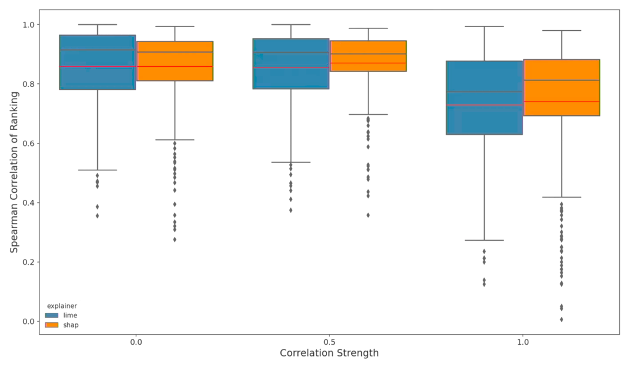
\includegraphics[width=0.7\textwidth]{experiment_details/media/image15.png}
\caption{Global ranking correlation of Explanations (LIME/SHAP) Between M and G Under Different Correlation Strength}
\label{fig:box_global}
\end{figure}


\textcolor{black}{To assess whether these discrepancies are structurally driven by data or model characteristics, we regress each evaluation metric on the five factors: \texttt{Num\_feature}, \texttt{Corr\_strength}, \texttt{Nonlinear\_num}, \texttt{Interaction\_num}, and \texttt{Accuracy}. In principle, this yields four heatmaps (two explainers $\times$ two correlation measures). Figure~\ref{heatmap_main} reports one representative result: the heatmap of factor regression using \textbf{SHAP} explanations and \textbf{Spearman} correlation. The other three heatmaps (LIME \& Spearman, LIME \& Kendall, SHAP \& Kendall) are relegated to Appendix~\ref{app:regression_results} as their conclusions are consistent with the one shown here. }


\textcolor{black}{Across metrics and explainers, we observe a consistent pattern: the four data-generation factors—\texttt{Num\_feature}, \texttt{Corr\_strength}, \texttt{Nonlinear\_num}, and \texttt{Interaction\_num}—tend to worsen the alignment between post hoc explanations and the ground truth (the corresponding cells are predominantly blue). In contrast, the \texttt{Accuracy} of $\mathcal{M}$ can partially improve alignment (red cells), but in practice managerial control over achieved accuracy is limited. Hence, even if higher accuracy offers some relief, the structural degradation induced by the underlying data characteristics remains the dominant force.}

\begin{figure}[h!]
\centering

\includegraphics[width=0.7\textwidth]{Rebuttal-R1/experiment_details/media/image37_v1.png}
\caption{Heat Map of Factor Regression Using SHAP \& Spearman (Combined Regression).}
\label{heatmap_main}
\end{figure}





% make matrix of results?
\section{Sensitivity Analyses}
    \label{sec:mitigation_strategies}
    \textcolor{black}{In this section, we use the results of our experiments and the implications of the theoretical results from Section \ref{sec:theoretical_considerations} to propose and test some means of altering what we will refer to as \emph{baseline} usage of explainers to see if alteration changes (improves) data alignment. If an alteration changes data alignment significantly, we will say that an explainer is sensitive to that alteration.} 
    
    A goal of this paper is to aid researchers by highlighting opportunities for improving use of post hoc explainers for hypothesis generation. As such, we are particularly interested in showcasing sensitive aspects of the pipeline that, when altered, may lead to increased data alignment. 
    
    This section attempts to identify sensitive aspects of both stages of the pipeline experimentally. We soften the impact of our choices for the data and model in the experiments by using the version of our loan approval dataset with mutually independent features and an NN with accuracy and test set ROC AUC equal to $.99$ in each experiment, unless otherwise stated. 

    %\subsection{sensitivity analyses for misalignment}
    %\label{sec:incorrectness_mitigation} %\textcolor{black}{move this to the end of section 4. this is the mitigation strategy for incorrectness}
    
        %We propose a few intuitive sensitivity analyses for explanation faithfulness based on data pre-processing and, model training, and explainer hyperparameters. We first demonstrate the truth of Corrolaries 1 and 2 from Section \ref{sec:theoretical_considerations}. We then verify that ensuring both that $\mathcal{M}$ has high test set accuracy and that its training data has no unobserved, correlated, or confounded features is associated with increased explanation quality. The next strategy involves ensuring that $\mathcal{M}$ has high test set ROC AUC. The final strategy involves ensuring that the underlying model of $\mathcal{E}$ correctly classifies the input being explained. When demonstrating the first, third, and fourth strategies, the training data do not have unobserved, correlated, or confounded features in order to isolate the roles of $\mathcal{E}$ and $\mathcal{M}$. 
   
    % DONT NEED HYPOTHESIS TESTING!
    % \subsection{Testing Improvement \textbf{\textcolor{black}{REMOVE OR REPOSITION???}}}
    %     \label{sec:improvement}
    %     This section introduces the hypothesis testing framework that we use to characterize whether an explanation method $\mE^\prime$ improves over a baseline explanation $\mE$ in terms of directionality, concordance, and relevance. All details, including statements of the null and alternative hypotheses we use, can be found in Appendix Section \ref{apx_sec:hypothesis_testing}.
        
        
    %     The underlying idea of our identification of improvement is to test if the mean(s) of metrics of interest is(are) higher for $\mE^\prime$ than for $\mE$ using Wilcoxon signed-rank tests on the location of mean of differences from  matched samples.
    %     %When testing for improvement of consistency of feature importance signs, we use one-sided McNemar tests for whether pairs of the pipeline with the mitigation strategy applied and baseline disagree on feature importance signs at the same rate. 
    %     All of our tests are performed with a significance level of $\alpha=.05$. 
        
    %     Our tests of improvement differ between concordance and directionality/relevance because the latter are feature-wise metrics. Since the computation of concordance involves all features, testing if it has been improved consists of a single Wilcoxon signed-rank test involving the matched pairs of concordances for each test instance. However, since directionality is computed for each feature and relevance is computed for $k=1,\ldots,D-1$, we formulate a rather strict characterization of improvement of $\mE^\prime$ over $\mE$ that takes into account the possibility that, e.g., $\mE^\prime$ may have higher relevance than $\mE$ for $k=1,2,3$ but lower relevance for $k=4$. Our tests for directionality and relevance are meant to capture when $\mE^\prime$ has a statistically significant improvement over $\mE$ in at least one respect and is not significantly worse than $\mE$ in any respect. What this means for directionality is that directionality must have a statistically significant increase for at least one feature and no statistically significant decrease for any feature. Similarly, for relevance, it means that the mean relevance of $\mE^\prime$ must be significantly larger than that of $\mE$ for at least one $k$, and not significantly smaller for any $k$.   
        
        
     


    
    
    \subsection{Explainer Specific Sensitivity Analyses}
        Before discussing general-use strategies, we present strategies applicable only to SHAP or LIME.% (but not both). 

            \subsubsection{SHAP Value Normalization}
                As discussed in Section \ref{sec:theoretical_considerations}, it follows directly from the theory underlying SHAP that SHAP explanations do not naturally extract the marginal effect values $\boldsymbol{\beta}$. It is therefore worthwhile to seek practical ways to modify our usage of SHAP. Since Equation (\ref{eqn:shap_gt}) showed that SHAP returns $e_{\text{SHAP}}(\mathbf{x}^{(i)})=\boldsymbol{\beta}^T(\mathbf{x}^{(i)} - \bar{\mathbf{x}})$ instead of $\boldsymbol{\beta}$, we proposed in Section \ref{sec:theoretical_considerations} to instead take the importance of feature $j$ to be $e_{\text{SHAP}}(x^{(i)}_j) / (x^{(i)}_j - \bar{x}_j)$ where $\bar{x}_j$ is the empirical mean of feature $j$ from the training data because this expression should be approximately $\beta_j$. Our experiments confirmed that SHAP explanations are not robust to normalization: Figure \ref{fig:shap_dividex_corr} showed that unmodified SHAP explanations perform about as well as random explanations with respect to our two metrics while the normalized SHAP explanations performed significantly better in all two metrics. Therefore, experiments involving SHAP will use SHAP normalization.% scheme by default.

                %In addition, the normalized SHAP explanations were more consistent across individuals (recall that Figure \ref{fig:shap_dividex_spearmans} showed that the concordance distribution for normalized SHAP explanations had a significantly smaller region of support which, importantly, was centered at a larger value than the mean concordance of the unmodified SHAP explanations). 
                %%Since these results were produced using the version of our dataset with correlated features, we additionally provide a comparison of SHAP without and with normalization when the input features are independent in Appendix Section \ref{apx_sec:shap_norm_indep}.



        
        \subsubsection{Changing LIME's Parameters} 
            \label{sec:lime_params}
             LIME is known to be unstable in the sense that its explanations are significantly affected by its parameters. In Appendix \ref{apx_sec:} we prove that LIME is sensitive to changes to the kernel bandwidth $\nu$ parameter and the number of perturbed samples $N$; these parameters need to be large in order for $e_{\text{LIME}}(x_j)$ to be close to $\boldsymbol{\beta}$. To show the impact of $\nu$ and $N$ experimentally, we compare the data-alignment of explanations from LIME explanations using the default choices of $\nu = .75\sqrt{D}$ (where $D$ is the number of features) and $N=1000$ used in the official LIME implementation \citep{ribeiro16lime} with explanations LIME explanations which use the larger values $\nu=N=10000$. 
            
            Figure \ref{fig:lime_tuning} demonstrates that LIME explanations are not robust to the number of samples $N$ and the kernel bandwith $\nu$ improved data-alignment. Note the large increases in directionality for ``Age," ``Cosigner," and ``Sex" and larger concordance associated with the larger $N,\nu$ values.  %For example, for directionality, increasing $\nu$ and $N$ improved directionality  significantly  ``Age," ``Cosigner," and ``Sex." The larger $\nu$ and $N$ also resulted in pairs of rankings whose concordances were significantly larger on average.
        
            \begin{figure}[ht!]
                \centering
                \begin{subfigure}[t]{.235\textwidth}
                  \centering
                  \captionsetup{justification=centering}
                      \raisebox{.2cm}{
\includegraphics[width=\textwidth]{Figures/sec4_4_lime-figure0.pdf}}%{Figures/lime_shap_Spearman_magnitude.png}
    
                  \caption{Directionality}%Spearman rank correlations of feature importance magnitudes from SHAP and LIME against the true ranking from $\mathcal{G}$. }
                   \label{fig:lime_tuning_sign_accs}
                \end{subfigure}%
                \hspace{.25cm}
                \begin{subfigure}[t]{.235\textwidth}
                  \centering
                   \captionsetup{justification=centering}
                  
\includegraphics[width=\textwidth]{Figures/sec4_4_lime-figure1.pdf}%{Figures/lime_shap_Spearman_signed.png}
                  \caption{Concordance}%Spearman rank correlations of signed feature importance from SHAP and LIME against the true ranking from $\mathcal{G}$.}
                   \label{fig:lime_tuning_spearmans}
                \end{subfigure}
                \hspace{.25cm}
                % \begin{subfigure}[t]{.28\textwidth}
                %   \centering
                %    \captionsetup{justification=centering}
                % 
\includegraphics[width=\textwidth]{Figures/sec4_4_lime-figure2.pdf}%
                % \caption{Relevance}%The average and standard error of recall of SHAP and LIME when attempting to capture the top K most important features to $\mathcal{G}$ when explaining $\mathcal{M}$, for varied $K=1,2,3,...$ number of features.}
                % \label{fig:lime_tuning_recalls}
                % \end{subfigure}
                \caption{Comparison of LIME explainer with default settings $\nu=.75\sqrt{D}\simeq 2.37,\ N=1000$ versus $\nu=N=10000$ with respect to our two metrics}
               \label{fig:lime_tuning}
            \end{figure} 
% \tw{Figure 8c looks so weird. How come it's a decreasing curve?}
            \subsubsection{Averaging Explanations of One Model by Different Explainers}
            \label{sec:averaging_one_explainer}
            As aforementioned, one of LIME's (potentially) problematic features is that, due to internal randomness (random seed, sampling, etc.), the feature importance it gives to the same instance for the same model can differ across runs \citep{alvarez18robustness}. 
            
        Researchers can easily check if their LIME explanations are not robust in the sense that qualitatively different explanations exist for their model by simply by re-running LIME with different parameters. Here, we propose that by checking if an explanation of a model constructed by averaging over a family of explanations of that model is qualitatively different than the individual explanations in the family, the averaged explanation may also have a quantitative difference in the sense of increased data alignment.
        
        Our experimental setup for this sensitivity analysis is as follows. Given a signgle model $\mathcal{M}$, for each of $M=100$ instances $\mathbf{x}$, we constructed averaged explanations by averaging the feature importance values given by 100 LIME explainers with different random seeds.
            %%To test this technique, we compare explanations averaged from 100 LIMEs with explanations from one LIME of $M=100$ applications. %The averaged explanation for each applicant is constructed by averaging over the feature importance values from 100 LIME explanations of the applicant, where the 100 explainers are created using random seeds $1,\ldots,100$ and default settings. .  %We repeat this with $\nu=n=10000$. 
            %%Our statistical tests of improvement concluded that directionality, concordance, and relevance were significantly improved by using averaged instead of single LIME explanations. 
            It is evident from our results, shown in Figure \ref{fig:lime_avg_sign_accs}, that the averaged LIME explanations had larger directionality values for ``Age," ``Sex," ``Married" and ``Cosigner." %The mitigation did not change the assignment of the other features but we were able to reject the null hypothesis of equal sign accuracies for ``Age," ``Cosigner," ``Married," and ``Sex" all with with $p<.001$. %$3.32e-3$, $2.34e-3$, $3.17e-5$, and $2.12e-6$, respectively.
            Furthermore, the concordances of the averaged explanations were significantly higher than those of the single explanations. %%Thus, when an explanation method has hyperparameters that affect the explanations it produces, it may be worthwhile to leverage the explanations of multiple instances of that explainer.%; we rejected the null hypothesis of equal concordances with $p<.001$.%a p-value of $7.39e-12$. %Figure \ref{fig:lime_avg_recalls} also shows that the averaged explanations were more likely to identify the features which were not the most or least important. 

            % \begin{table}[]
            % \centering
            % \begin{tabular}{|l|l|l|l|l|l|l|l|l|l|}
            % \hline
            % Age  & Cosigner & Credit History & Credit Score & Delinquency & Income & Inquiries & Married & Sex & Utilization \\ \hline
            % 0.98 & 1.20e-7   & n/a            & n/a          & n/a         & n/a    & 0.50      & 1.11e-4 & .12 & n/a         \\ \hline
            % \end{tabular}
            % \caption{p-values for improvement to consistency of feature importance signs by using averaged LIME explanations. Values are listed as ``n/a" if both pairs of explanations always found the correct sign for the corresponding feature.}
            % % \label{tab:lime_avg_sign_con}
            % \end{table}
                             
            \begin{figure}[!h]
            \centering
                \begin{subfigure}[t]{0.235\textwidth}
                \centering
                \raisebox{.2cm}{
\includegraphics[width=\textwidth]{Figures/sec5_2_lime_avg-figure0.pdf}}
                \caption{Directionality} \label{fig:lime_avg_sign_accs}
            \end{subfigure}\hspace{.25cm}
            \begin{subfigure}[t]{0.235\textwidth}
                \centering
                \raisebox{.05cm}{
\includegraphics[width=\textwidth]{Figures/sec5_2_lime_avg-figure1.pdf}}
                \caption{Concordance} \label{fig:lime_avg_spearmans}
            \end{subfigure}\hspace{.25cm}
            %  \begin{subfigure}[t]{0.28\textwidth}
            %     \centering
            %     
\includegraphics[width=\textwidth]{Figures/sec5_2_lime_avg-figure2.pdf}
            %     \caption{Relevance}
            %     \label{fig:lime_avg_recalls}
            % \end{subfigure}
            \caption{Comparisons of results for our two metrics for  explanations of an NN $\mathcal{M}$ by 1 LIME explainer versus those created by averaging the feature importance values of 100 LIME explanations of $\mathcal{M}$}\label{fig:lime_avg}
            \end{figure}

                
            %It was also the case that the averaging routine significantly improved consistency. To obtain this result, we created another set of average explanations from 100 more LIME explainers using random seeds $101,\ldots,200$, and tested whether the signs and rankings were more consistent between the two sets of averaged explanations compared to the signs and rankings of the two individual LIME explainers. We rejected the null hypotheses of our tests for equal consistency of feature importance signs in favor of improvement for ``age", ``cosigner", and ``married" all with $p<.001$.%of  $8.65e-3$, $1.20e-7$ and $1.11e-4$, respectively.
            %There was no change for ``credit  history", ``credit score", ``delinquency", ``income", and ``utilization" because both methods were perfect in each case.  With a p-value of $7.60e-15$, we rejected the null hypothesis of our Wilcoxon test that the means of the two concordance distributions are equal in favor of the alternative hypothesis that the mean of the concordance distribution from the averaged explanations is larger. That this is the case is also visually evident from Figure \ref{fig:lime1_v_100_incon}; the concordance distribution of the averaged explanations was more concentrated near 1 and its tail was also shorter. 

            % \begin{figure}[ht!]
            %     \centering
            %     %\begin{subfigure}{.3\textwidth}
            %       \centering
            %       \captionsetup{justification=centering}
            %       
\includegraphics[width=.28\textwidth]{Figs/sec5_2_lime_avg2-figure3.pdf}
            %       \caption{Comparison of concordances between explanations from pairs of individual LIME explainers and between pairs of averaged explanations from two sets of 100 LIME explainers.}%Spearman rank correlations of ranked feature importance magnitudes from LIME against the true ranked magnitudes from $\mathcal{G}$.}
            %        %\label{fig:lime_income}
            %     %\end{subfigure}%
            %     %\caption{}%Violin plots of feature importance values for \emph{income} from SHAP and LIME for cases when \emph{income} is unconfounded and confounded by the unobserved social support feature}
            %     \label{fig:lime1_v_100_incon}
            % \end{figure}
                
    \subsection{General Sensitivity Analyses}
        We now suggest some means of checking whether a given post-hoc explanation can be substantially improved. Note that we have been and will continue using normalized Shapley values, since default SHAP explanations are not better than random with respect to data-alignment. %To show the utility of these strategies for SHAP, we will use normalized SHAP values in each the experiments below. 

        \subsubsection{Putting Occam's Razor into Practice}
            \label{sec:decreasing_complexity}
            Hypothesis spaces, which are sets of all possible machine learning models of a given type(s), are in practice unimaginably large, making model selection challenging from the outset. Further complicating this process is the aforementioned Rashomon effect. Given that notions of complexity, such as parameter count, are fundamental distinguishing properties of models, the statistics literature on parsimony in curve fitting often appeals to Occam's razor—plurality should not be posited without necessity—suggesting that simpler models are more likely to be correct than complex ones \citep{popper2005logic}. For this reason, we %%designed a mitigation strategy that takes into account the complexity of $\mathcal{M}$. As we established in Section \ref{sec:role_of_predictive_power}, there is an association between the predictive performance of $\mathcal{M}$ and the alignment of post hoc explanations of $\mathcal{M}$ with respect to $\mathcal{G}$. This mitigation strategy 
            propose and test the idea that stage 1 is sensitive to model complexity. %in addition to finding an especially well-performing model $\mM_1$, researchers also find a set of simpler models $\mathcal{M}_2,\mathcal{M}_3,\ldots$ whose performance is reasonably close to that of $\mathcal{M}_1$. 
 %The labels predicted by $\mathcal{M}$ (after thresholding its output probabilities) agreeing with those in the test set is an incomplete representation of faithfulness to $\mathcal{G}$; even if $\mathcal{M}$ had 100\% training and testing accuracy on data with no measurement error, this does not mean $\mathcal{M}=\mathcal{G}$.  Thus, it is worth making an effort not to over-parameterize $\mathcal{M}$. %\tw{The explanation should be moved to earlier this paragraph. WE can use the argument of Ocam's razor, that low complexity is generally preferred. This point should be given a deeper discussion before proposing to get ``minimal complexity"} 
 
            A simple way to perform this sensitivity analysis is to iteratively train and evaluate models of successively lower complexity, stopping the process once a reduction in complexity results in a significant decrease in predictive performance.
   \begin{figure}[t!]
            \subfloat[SHAP Dir.]{%
                \raisebox{.2cm}{
\includegraphics[width=.22\textwidth]{Figures/sec5_mlp_complexity_shap-figure0.pdf}}%
                \label{subfig:decreasing_complexity_shap_sign_accs}%
            }\hspace{.25cm}
            \subfloat[SHAP Conc.]{%
                \raisebox{.05cm}{
\includegraphics[width=.22\textwidth]{Figures/sec5_mlp_complexity_shap-figure1.pdf}}%
                \label{subfig:decreasing_complexity_shap_spearmans}%
            }\hspace{.25cm}
            % \subfloat[SHAP Relevance]{%
            %     
\includegraphics[width=.28\textwidth]{Figures/sec5_mlp_complexity_shap-figure2.pdf}%
            %     \label{subfig:decreasing_complexity_shap_recalls}%
            % }\\
            \subfloat[LIME Dir.]{%
                \raisebox{.2cm}{
\includegraphics[width=.22\textwidth]{Figures/sec5_mlp_complexity_lime-figure0.pdf}}%
                \label{subfig:decreasing_complexity_lime_sign_accs}%
            }\hspace{.25cm}
            \subfloat[LIME Conc.]{%
                \raisebox{.05cm}{
\includegraphics[width=.22\textwidth]{Figures/sec5_mlp_complexity_lime-figure1.pdf}}%
                \label{subfig:decreasing_complexity_lime_spearmans}%
            }
            % \hspace{1cm}
            % \subfloat[LIME Relevance]{%
            %     
\includegraphics[width=.28\textwidth]{Figures/sec5_mlp_complexity_lime-figure2.pdf}%
            %     \label{subfig:decreasing_complexity_lime_recalls}%
            % }\\
            \caption{Comparisons of results for our two metrics for SHAP (top row) and LIME (bottom row) explanations of equally accurate NNs with high and low complexity.}
            \label{fig:decreasing_complexity}
        \end{figure}
        
            The settings of our implementation of this check are as follows. The first NN, $\mathcal{M}_1$, has 100 nodes in its hidden layer (the default in sklearn) and achieves a test set AUC of about 0.99. The second, simpler NN, $\mathcal{M}_2$, has just two hidden nodes, yet it still achieves a test set AUC of around 0.98. 
            
            Figure \ref{fig:decreasing_complexity} visualizes our comparison of the explanations provided by SHAP and LIME for $\mathcal{M}_1$ and $\mathcal{M}_2$. %Additional results and further motivation for this strategy can be found in Appendix Section \ref{apx_sec:appendix_inconsistency}.
            We found that, by explaining the simpler NN $\mathcal{M}_2$ instead of the more complex $\mathcal{M}_1$, it was possible to get more data-aligned explanations. %However, as shown by Figure \ref{fig:decreasing_complexity}, the improvements were marginal for the most part. \textcolor{black}{I don't think so. let's talk about it}. 
            In particular, SHAP's directionality for ``Age and ``Credit History."%% as well as SHAP's relevance for $k=1,2,4,5,6,7$ were increased significantly. 
           %For SHAP, we reject the null hypothesis of equal sign accuracies only for ``Age" with $p<001$ and ``Credit History" with a p-value of $0.04$. It is evident from Figure \ref{subfig:decreasing_complexity_shap_spearmans} that concordance did not rise significantly; we failed to reject the null hypothesis of equal concordances with a p-value of $.16$. Although relevance worsened for $k=8$ when explaining $\mathcal{M}_2$, the small improvements for $k=1,2,4,5,6,7$ were all statistically significant with $p<.001$ except for $k=4$, which had $p=.05$. 
            For LIME, directionality was improved for ``Married," concordance was significantly improved overall.%%, and relevance was significantly increased for $k=2,6$. %%Overall, these results suggest that explanations of simpler models can be more data-aligned than explanations of more complex models with equivalent predictive performance. 

            
            %For LIME, we could only conclude that the directionality of ``Married" improved by rejecting the null hypothesis of equal directionality with a p-value of $0.015$. However, the improvement to concordance was significant, as its test had $p<.001$. As for relevance, the results for $k=1$ were identical and the null hypothesis of equal relevance was rejected in favor of improvement for $k=2,6$ with p-values of $0.02$ and $0.01$. Overall, the results suggest that explanations of simpler models are more data-aligned than explanations of more complex models with equivalent predictive performance. 
            
            A reason that the explanations of the simple model $\mathcal{M}_2$ were more data-aligned is that even though $\mathcal{M}_1$ and $\mathcal{M}_2$ may have similar behavior in how they generate training and test set label predictions, the additional expressive power of $\mathcal{M}_1$ allows the local behavior of its decision boundary to be more erratic. Given that SHAP and LIME are local function approximators, incorrect local behavior of $\mathcal{M}_1$ limits how data-aligned SHAP and LIME can be when explaining $\mathcal{M}_1$. 

            
       

        \subsubsection{Accounting for the Rashomon Effect: Averaging Explanations of Different Models}
           %The rapid proliferation of new machine learning models and methods has made it increasingly challenging for researchers to decide which model to use and ultimately explain. Based on the Rashomon set theory \citep{semenova22rashomon,wang2022timbertrek,donnelly2023rashomon}
           A straightforward approach to checking how robust post hoc explanations of data are to the choice of model is to train multiple models, generate explanations for each, and then average those explanations. This idea, which is motivated by literature on Rashomon sets \citep{semenova22rashomon,wang2022timbertrek,donnelly2023rashomon},  incorporates diverse information from the hypothesis space into the final (averaged) explanation.


            We demonstrate this sensitivity analysis by repeating the experiments of Section \ref{sec:evaluating_faithfulness} twice: first using explanations for a single model, and then averaging explanations for 10 unique neural networks (NNs) with ROC AUC scores of at least 0.9. The averaged explanations are constructed separately for SHAP and LIME in the following manner. Given an applicant, one explanation is created for each NN. The resulting 10 feature importance vectors are then averaged.%% We aim to test whether these averaged explanations offer an improvement over singular explanations.% in terms of data-alignment.
            % PUT THESE DETAILS IN APPENDIX
            %Each NN is trained with 5 hidden layers and for 10 iterations as before, but each NN initializes its training with a different random seed. We control for the inconsistency of the explainers by using default hyperparameters and keeping the random seed of the explainers the same. 
             
            Our experimental results suggest that an opportunity may exist, mainly for LIME, to increase data-alignment using feature importance averaging strategies.% but the results of our Wilcoxon tests for improvement of data-alignment were not consistent between SHAP and LIME. The differences are visualized in Figure \ref{fig:mlp_increase}. 
             Regarding SHAP, Figures \ref{subfig:mlp_avg_shap_sign_accs} and Figure \ref{subfig:mlp_avg_shap_spearmans} show that there was a large improvement in directionality for ``Age" and small improvements in directionality for many other features. However, concordance for the SHAP-based pipeline seemed to be for the most part robust to importance averaging. Showing a stark contrast with SHAP, LIME's directionality and concordancewere both significantly improved. %%Given these results, we can only adduce that this strategy is effective for LIME.  %Directionality for the other features was perfect for the other features both with and without the mitigation. In contrast, for SHAP, there was no significant change to directionality for any feature, no significant change to concordance, and no significant change to relevance for any $k$.  Given these results, we can only adduce that this strategy is effective for LIME. In particular, it was effective in increasing directionality and concordance, but not relevance.  %Our results are shown in Figure \ref{fig:mlp_increase}.
            
            %Figure \ref{subfig:mlp_avg_lime_spearmans} shows that LIME's averaged explanations had a slightly larger mean and slightly lower range while Figure \ref{subfig:mlp_avg_lime_spearmans} shows that concordance was almost unchanged for SHAP. Figures \ref{subfig:mlp_avg_lime_sign_accs} and  for LIME and \ref{subfig:mlp_avg_shap_sign_accs} and \ref{subfig:mlp_avg_shap_recalls} show that, with a few exceptions, the averaged explanations were at least as good as the explanations of a single model at identifying feature importance signs and the top-$k$ features. 
            
            %However, the strategy does not seem to be particularly beneficial for finding the top-$k$ features; the curves plotting the recall for SHAP and LIME in Figures \ref{subfig:mlp_avg_lime_recalls} and \ref{subfig:mlp_avg_shap_recalls} are nearly identical for the averaged and single explanation.%Figure \ref{fig:mlp_avg_recalls} also shows that the curves representing the relationships between $K$ and recall for $n=100$ bound the other curves from above. Therefore, this strategy appears to be effective in reducing both misalignment and inconsistency.

            % This strategy can be seen as a simplified version of \citep{donnelly2023rashomon}. Instead of leveraging explanations of good models trained on one dataset, they leverage explanations of optimal decision trees or GAMs trained on bootstraps of one dataset. At the time of writing, their method is not valid for more complex models like neural networks. It also produces statistics for feature importance instead of singular feature importance values. 
    

        \begin{figure}[t!]
            \subfloat[SHAP Dir.]{%
                \raisebox{.2cm}{
\includegraphics[width=.22\textwidth]{Figures/sec5_2_mlp_avg_shap-figure0.pdf}}%
                \label{subfig:mlp_avg_shap_sign_accs}%
            }\hspace{.25cm}
            \subfloat[SHAP Conc.]{%
                \raisebox{.05cm}{
\includegraphics[width=.22\textwidth]{Figures/sec5_2_mlp_avg_shap-figure1.pdf}}%
                \label{subfig:mlp_avg_shap_spearmans}%
            }\hspace{.25cm}
            % \subfloat[SHAP Relevance]{%
            %     
\includegraphics[width=.28\textwidth]{Figures/sec5_2_mlp_avg_shap-figure2.pdf}%
            %     \label{subfig:mlp_avg_shap_recalls}%
            % }\\
            \subfloat[LIME Dir.]{%
                \raisebox{.2cm}{
\includegraphics[width=.22\textwidth]{Figures/sec5_2_mlp_avg_lime-figure0.pdf}}%
                \label{subfig:mlp_avg_lime_sign_accs}%
            }\hspace{.25cm}
            \subfloat[LIME Conc.]{%
                \raisebox{.05cm}{
\includegraphics[width=.22\textwidth]{Figures/sec5_2_mlp_avg_lime-figure1.pdf}}%
                \label{subfig:mlp_avg_lime_spearmans}%
            }
            % \hspace{1cm}
            % \subfloat[LIME Relevance]{%
            %     
\includegraphics[width=.28\textwidth]{Figures/sec5_2_mlp_avg_lime-figure2.pdf}%
            %     \label{subfig:mlp_avg_lime_recalls}%
            % }\\
            \caption{Comparisons of data-alignment for SHAP (top row) and LIME (bottom row) explanations of 1 NN versus explanations constructed by averaging the feature importance values of 10 NNs.}
            \label{fig:mlp_increase}
        \end{figure}
        

   
    
    \subsection{Summary and Discussion of Sensitivity Analyses}
            \label{sec:summary_and_strategies}
             Our investigation of sensitivity analyses suggests that SHAP and LIME are sensitive to several alterations in their usage that can increase data alignment. Stage 1 is not robust because a family of models yields a family of explanations, each of which is different than the average explanation (over the family). Stage 2 is also not robust. SHAP's ability to extract marginal effects is sensitive to SHAP value normalization. LIME is sensitive to increases in $\nu$ and $N$, as well as its random seed. 
             
             %%For LIME, it may be beneficial to aggregate the explanations from multiple LIME instances, with each individual LIME explainer configured with large values for $\nu$ and $N$. Additionally, it is recommended to select black box models that strike an optimal balance between complexity and predictive power, and to average explanations across ensembles of explainers and/or models.
            %It makes less sense to combine explanations of a single model than explanations of multiple models because of the idea that ``all models are wrong." 

            %%We discuss two unsuccessful sensitivity analyses in the Appendix, both based on aggregating explanations of a single black box. The first exchanges the previously used simple averaging of LIME explanations for a method of ranked choice voting known as the Borda count and the second averages SHAP and LIME explanations together. We believe that a core reason why these two strategies were unsuccessful is that they only involve a single black box model. Finding common (valid) patterns within multiple black boxes is possible by aggregating explanations of those models, whereas aggregations of explanations of a single black box can at best reveal the single, imperfect, pattern identified by that black box. Ignoring bias and error in the dataset, each explanation has two layers of approximation error with respect to the ground truth, whereas each black box has only its own approximation error and captures different patterns in the training data. Thus, researchers may find averaging feature importance values obtained by many models both a useful and intuitive strategy \citep{dong2020variable,donnelly2023rashomon}.  %With the configuration of data and model we used, the local error rates of both SHAP and LIME were skewed to the right, implying that the mean local fidelity over samples of SHAP and LIME models can decrease as the sample size increases. However, it is difficult to validate this claim because the local fidelity of SHAP and LIME is not an especially good measure of how faithful their explanations are to $\mathcal{G}$. That averaging SHAP and LIME together did not yield a consistent and substantial advantage is likely due to the simplicity of the technique. For this reason, we suggest that more research be done on this topic. 
            
            %%Researchers who would like to investigate the importance and impact of features in the data may find exploring the following general strategy useful.
        %First, the choice of explainer(s) used for the strategy should be guided by user preference for the types of feature importance outlined in Section \ref{sec:theoretical_considerations}. For example, LIME should be preferred to SHAP if  $\boldsymbol{\beta}$ is considered to be the ground truth feature importance representation.  %construct average explanations over a collection of good LIME explanations of good models. If situational importance is more suitable than theoretical importance for the application, researchers should instead average over SHAP explanations of good models. 
            %%When starting the prediction stage, the dataset should be pre-processed to remove highly correlated features.\footnote{If possible, adjustments can be made to account for confounding. Tools like E-values\citep{gaster2023quantifying} and Pearl's backdoor criterion can be used for this purpose.} % The causal graph can be estimated using Bayesian Networks if sufficient domain knowledge is available.}
            %%Having pre-processed the data, researchers are encouraged to train $B\geq 1$ black box models with simple enough decision boundaries to not lose too much predictive performance compared to more complex models.\footnote{Ideally, Rashomon sets of models would be constructed and the simplest models in them would be collected.} To construct a more robust explanation of a model's predicted outcome for an instance, the results of multiple explainers of that model can be aggregated by, e.g., averaging the feature importance values for each feature over the explainers. An even more robust final explanation for an instance can be produced by averaging over the importance values given in the $B\times E$ explanations of the predictions of $B$ models by $E$ explainers.
          


% \subsection{Case Study Using Real Data and Econometric Method} \textbf{\textcolor{black}{REMOVE OR REPLACE???}}
%     \label{sec:case_study}
%     To validate the efficacy of our sensitivity analyses and demonstrate their practical application, we test whether they provide an advantage over the default usage of SHAP and LIME in extracting the same marginal effects as those identified in an econometric study on home loan application approvals \citep{bane2006econometric}. Specifically, we will adapt the framework outlined in Section \ref{sec:summary_and_strategies} to create mitigated pipelines for SHAP and LIME separately.
    
%    The home loan dataset is publicly available and originates from a study by the Federal Reserve Bank of Boston \citep{hunter1996cultural}. We consider the ground truth $\boldsymbol{\beta}$ to be the coefficients of the logistic regression model obtained in \cite{bane2006econometric}'s analysis of that dataset. This assumption is justifiable because econometric modeling is well-suited to capture $\boldsymbol{\beta}$. The linear ground truth model derived from their logistic regression model is presented in Equation (\ref{eqn:econ_gt}), and the meanings and ranges of each feature are provided in Table \ref{apx_tab:case_study_features} in the Appendix.  %We will use the logistic regression coefficients to evaluate SHAP and LIME explanations in the same manner as has been done throughout this paper. We suppose that the logistic regression coefficients have the correct signs and magnitudes relative to each other, not that the logistic regression itself is the true causal model underlying home loan approvals in Boston. 

%     %\begin{tcolorbox}[title = Econometric Ground Truth Model $\mathcal{G}$]
%     \begin{equation}
%     \label{eqn:econ_gt}
%     \begin{split}
%         \mathcal{G}(X) =.8 + 3.5\cdot \text{good credit} + 4.7\cdot \text{purchaser type} -4.4 \cdot \text{PMI approved} - .4 \cdot \text{multi family} \\ -2.5 \cdot \text{unver} + .9 \cdot \text{fixed rate} - 1.4 \cdot \text{bankruptcy} - .9 \cdot \text{value rate} - .03 \cdot \text{debt rate} \\- .7 \cdot \text{old} + .8 \cdot \text{married} - .8 \cdot \text{gift}.
%     \end{split}
%     \end{equation}
%     %\end{tcolorbox}
%     %\subsection{Baseline Performance}
%     %Figure \ref{fig:econ_cmp} compares the explanation quality  for 100 applicants from the baseline pipeline and recommended pipeline. %In the Appendix, we show also compare results for importance sign accuracy, Spearman rank correlation, and recall.
    
% Our mitigated pipelines for SHAP and LIME are applications of the mitigation framework outlined in Section \ref{sec:summary_and_strategies}. First, we split the dataset into 80\% training data and 20\% testing data. Then, we trained a family of 210 neural networks (NNs) using a parameter grid with hidden layer nodes ranging from 2 to 100 and random seeds from 1 to 10. From this family, we selected the 10 NNs with the fewest hidden layer nodes that also achieved a test set AUC no more than $\epsilon = 0.02$ lower than the highest AUC observed within the family (.93). For each of these 10 NNs, we produced $E = 10$ SHAP and LIME explainers.

% The mitigated LIME pipeline utilizes all 10 NNs, with 10 LIME explainers for each NN. Each LIME explainer is configured with $\nu = N = 10,000$. Since SHAP is deterministic and the NN averaging strategy did not significantly improve directionality and concordance for SHAP, we use $B = E = 1$ for SHAP and normalize the Shapley values. For comparison, baseline explanations are derived from a single NN with an accuracy of 0.86 and a ROC AUC of 0.93, using individual SHAP and LIME explainers with default settings.




%     Both the SHAP and LIME variants of our general strategy showed improvements over the baseline in at least one respect. These improvements are illustrated in Figure \ref{fig:econ_cmp}. Specifically, our strategy applied to SHAP significantly enhanced directionality for all features except two (``gldin" and ``gift") and also substantially improved both concordance and relevance. When applied to LIME, our strategy significantly improved overall concordance, greatly enhanced directionality for the features ``fixadj," ``gift," and ``obrat," and significantly increased relevance for the top 2, 3, and 4 features.%It had worse directionality only for ``vr" and ``obrat," and worse relevance for features not in the top-4. 

%     %%\textcolor{black}{what are the econometric insight? we might have been overclaiming}
%     %Figure \ref{fig:econ_cmp} visualizes the results. The directionality values from our recommended strategy with SHAP and LIME were at least as good as those from the baseline for all features except ``pubrec" (bankruptcy filed) for LIME and ``vr" (value rate) for SHAP (see Figures \ref{subfig:econ_lime_sign_accs} and \ref{subfig:econ_shap_sign_accs}). The concordance plots for both SHAP and LIME in Figures \ref{subfig:econ_shap_spearmans} and \ref{subfig:econ_lime_spearmans} show that the recommended pipeline rankings were generally more faithful than the most faithful explanations from the equivalent baseline. Finally, it can be seen from Figures \ref{subfig:econ_lime_recalls} and \ref{subfig:econ_shap_recalls} that the recommended strategies using SHAP and LIME both have substantially higher relevance for all $k\neq 1,\ 10,\ 11$.
     
% % \begin{figure}[!h]
% % \centering
% %     \begin{subfigure}[t]{0.28\textwidth}
% %     \centering
% %     
\includegraphics[width=\textwidth]{Figs/econ_cmp-figure0.pdf}
% %     \caption{Directionality} \label{fig:econ_cmp_sign_accs}
% % \end{subfigure}\hspace{1cm}
% % \begin{subfigure}[t]{0.28\textwidth}
% %     \centering
% %     
\includegraphics[width=\textwidth]{Figs/econ_cmp-figure1.pdf}
% %     \caption{Relevance} \label{fig:econ_cmp_spearmans}
% % \end{subfigure}\hspace{1cm}
% %  \begin{subfigure}[t]{0.28\textwidth}
% %     \centering
% %     
\includegraphics[width=\textwidth]{Figs/econ_cmp-figure2.pdf}
% %     \caption{Recall}
% %     \label{fig:econ_cmp_recalls}
% % \end{subfigure}
% % \caption{Improvements due to use of recommended pipeline instead of one without any of our sensitivity analyses}\label{fig:econ_cmp}
% % \end{figure}


%         \begin{figure}[t!]
%             \subfloat[SHAP Directionality]{%
%                 \raisebox{.2cm}{
\includegraphics[width=.28\textwidth]{Figures/shap_econ-figure0.pdf}}%
%                 \label{subfig:econ_shap_sign_accs}%
%             }\hspace{1cm}
%             \subfloat[SHAP Concordance]{%
%                 \raisebox{.05cm}{
\includegraphics[width=.28\textwidth]{Figures/shap_econ-figure1.pdf}}%
%                 \label{subfig:econ_shap_spearmans}%
%             }\hspace{1cm}
%             \subfloat[SHAP Relevance]{%
%                 
\includegraphics[width=.28\textwidth]{Figures/shap_econ-figure2.pdf}%
%                 \label{subfig:econ_shap_recalls}%
%             }\\
%             \subfloat[LIME Directionality]{%
%                 \raisebox{.2cm}{
\includegraphics[width=.28\textwidth]{Figures/lime_econ-figure0.pdf}}%
%                 \label{subfig:econ_lime_sign_accs}%
%             }\hspace{1cm}
%             \subfloat[LIME Concordance]{%
%                 \raisebox{.05cm}{
\includegraphics[width=.28\textwidth]{Figures/lime_econ-figure1.pdf}}%
%                 \label{subfig:econ_lime_spearmans}%
%             }\hspace{1cm}
%             \subfloat[LIME Relevance]{%
%                 
\includegraphics[width=.28\textwidth]{Figures/lime_econ-figure2.pdf}%
%                 \label{subfig:econ_lime_recalls}%
%             }\\
%             \caption{Improvements due to use of recommended pipeline instead of one without any of our sensitivity analyses}\label{fig:econ_cmp}
%         \end{figure}
%     %\tw{Figure 12 (f) makes our strategies less convincing. The result looks weird. Did you double check?}





\section{Discussion and Conclusion}
    \label{sec:discussion}
    As post hoc explanations are gaining popularity in business research, we found an alarming trend of using them to make claims about the marginal effects of variables in the data.  However, the validity of this use of post hoc explanations has not been studied in the literature. 
    Our paper is the first effort towards this purpose. 
     In the following sections, we will summarize our findings and give some parting advice for the use of post hoc explainers for obtaining data insights in business research. 
    We also contribute to the business literature by proposing some simple and intuitive sensitivity analyses which show various ways in which both stages of the pipeline are sensitive to inputs and parameters. 
    %    
    %In this paper we have introduced and investigated issues of misalignment and inconsistency of post hoc explanations. Our thorough literature review uncovered that business researchers using post hoc explanations value data-alignment. Thus we have contributed to the business literature by providing both theoretical and empirical evidence that the two most popular explainers, LIME and SHAP, often produce misaligned explanations. Notably, we proved that SHAP is inherently unsuitable to infer information about $\boldsymbol{\beta}$. %We have also identified various factors that contribute to misalignment and inconsistency. 


    \subsection{Main Findings}
        We contribute several important findings to the use of post hoc explanations in business research.

            First, through an extensive literature review, we found that the use of post hoc explanations to infer information about the data is quite prevalent. In the 150 papers we reviewed, 63 used SHAP or LIME to draw conclusions about the $X\rightarrow Y$ relationship instead of the $\mathcal{M}(X)\rightarrow \hat{Y}$ relationship. Such use deviates from the intended purpose of post hoc explainers; they are designed to explain the machine learning model, not to extract information about the data. Identifying this misuse of post hoc explanations is an important contribution of this paper. Note that while post hoc explanations have been first introduced and widely used in the machine learning community, the issue we discuss in this paper is less of a concern for that community because computer scientists are more interested in explaining the machine learning models. They use post hoc explainers to understand a model's behavior in order to diagnose and debug the model. However, the goal of business researchers is to understand the data and the underlying phenomena, making this issue more pertinent in business research.
        % Using simulated loan application datasets, we produced ground truth application approval mechanisms $\mathcal{G}$ along with NN approximators $\mathcal{M}$ trained on $\mathcal{G}$ and investigated how well popular post hoc explainers could recover the $\boldsymbol{\beta}$ underlying $\mathcal{G}$. This investigation was motivated by the need to assess the utility of post hoc explainers to business researchers and managers. We used our results from the investigation using simulated data to propose a set of mitigations that would worth exploring in practice. Finally, we tested the efficacy of this set of mitigations in a test to see if we could use LIME to reproduce the results of an econometric study of home loan applications. We found that although it was far better to use them than not, the resulting explanations were still imperfect. 

        % When evaluating the ability of the two most popular post hoc explainers, SHAP and LIME, to extract faithful insights from both real and simulated data, we identified the following issues that are cause for concern for researchers interested in $\boldsymbol{\beta}$ estimation problems using post hoc explainers. 

       Second, we provide both theoretical and empirical evidence that SHAP and LIME explanations are, in fact, generally not data-aligned \textcolor{black}{even when the ground truth being learned by $\mathcal{M}$ is just a linear model. In our investigation, we showed that SHAP and LIME explanations of a black box model tasked with learning from data sampled from a linear ground truth model incorrectly represent the signs and relative importance of the marginal effects of the explanatory variables. Furthermore, we showed that SHAP and LIME fail to be informative about four common notions of feature importance in general.} As shown in Section \ref{sec:causes_of_misalignment}, SHAP and LIME tend to be data-misaligned even in scenarios where they explain an accurate machine learning model trained on data whose features are mutually independent and whose target is derived from a simple linear ground truth model - scenarios which are, in a sense, ideal. This observation suggests a need for caution when interpreting variable relationships based on post hoc explanations. It opens up a dialogue about the complexities of deriving accurate insights from machine learning models via post hoc explainers, contributing to a deeper understanding of their limitations and paving the way for future research in this area. In light of these insights, it may be beneficial for the academic community to revisit prior analyses that have relied heavily on post hoc explanations. This reassessment could ensure that interpretations and conclusions drawn from such models are robust and reflective of their underlying dynamics. Our findings underscore the importance of continuous critical evaluation in the field, especially as we seek to refine our understanding and application of these tools. 
        
        \textcolor{black}{Third, we identify different causes of SHAP and LIME's lack of data-alignment. Achieving data-alignment is made impractical at the outset due to the Rashomon effect, since it is extremely unlikely that even a well performing $\mathcal{M}$ represents the same decision process as $\mathcal{G}$. Additionally, we showed that due to the nature of Shapley values, SHAP is inherently unable to report marginal effects.} Shapley values represent a feature's contribution to a prediction by considering not only the feature's marginal effect but also its value and the influence of other variables within the explanation process. In the particular case where SHAP explains a linear model, the vector of Shapley values is given by $\boldsymbol{\beta}(\boldsymbol{\xi}-\bar{\mathbf{x}})$, diverging from a direct representation of $\boldsymbol{\beta}$. Moreover, LIME's data-misalignment arises from the mechanics of its default ridge regression approach. Our analysis, supported by Theorem \ref{thm:lime_thm}, indicates that LIME could achieve data-alignment by avoiding the discretization of numerical inputs, sampling many points for its synthetic regression problem, and opting for a significantly larger bandwidth than the default. Yet, even with these adjustments, common properties of real-world data such as correlated variables often hinder the attainment of data-alignment. Nonetheless, it is noteworthy that our evaluations generally reveal \textit{LIME to provide explanations more aligned with the ground truth compared to SHAP}.
 
        
         Finally, we identify several sensitivity analyses that show promise in enhancing the data-alignment of explanations across various stages of the explanation pipeline. These strategies, validated through empirical testing, offer significant improvements in aligning explanations more closely with marginal effects. However, it is important to acknowledge that none of the strategies can guarantee complete congruence with marginal effects. This absence of a full guarantee means that while explanations may sometimes align closely with the marginal effects, they cannot reliably do so. Such a scenario potentially restricts the applicability of post hoc explanations for extracting data insights, as users may remain uncertain about the extent to which these explanations accurately mirror the underlying the marginal effect structure. This limitation underscores the need for cautious interpretation and application of post hoc explanation methods in practical scenarios.
        
        
        % \textcolor{black}{what else did we *find*?}

            
        % Second, users must deal with inconsistent explanations because not only do e.g. SHAP and LIME each produce different explanations for the same outcome, but LIME may produce self-contradictory explanations of the same outcome. How to select an explanation(s) from the myriad available from different combinations of accurate black box models, explainers, and explainer hyperparameters is up to the user, but the mitigations suggested in this paper can help users make more informed decisions.%but sensitivity analyses like those presented in this paper can be used to estimate how confident users can be in their selection(s). 



        % stuff re: prescriptive removed
        %Our main finding regarding prescriptive insights is that LIME, SHAP, and DiCE seem to only be of use for actionable recourse a minority of the time. When tasked with generating new application profiles for denied loan applicants, those new application profiles would be approved by $\mathcal{G}$ less than 50\% of the time. %\textcolor{black}{May need to be removed!! We showed that... DiCE, a counterfactual explainer (as opposed to an attributive one like SHAP and LIME) was always able to produce new application profiles for rejected loan applicants that would lead to approval in our experiments (for a sufficiently small sparsity parameter). }For DiCE, if we restrict the range of feature variations (within one standard deviation) and the number of features allowed to vary, it can only provide prescriptive insights to a small number of denied applicants.
        
    % \subsection{On sensitivity analyses}
    %     We proposed some intuitive sensitivity analyses for the issues of unfaithful and inconsistent explanations. Each of them was effective with respect to at least one of our three metrics. However, none of them were fully effective solutions that would guarantee that practitioners could confidently use LIME or SHAP for $\boldsymbol{\beta}$ estimation and econometric modeling. Thus, we encourage cautionary usage of SHAP and LIME and to consider exploring the usage of our sensitivity analyses in efforts to obtain more data-aligned explanations. 
        
    %     Our principal finding regarding faithfulness was that SHAP has no chance at data-alignment unless its Shapley values are normalized by the difference between feature values and feature means. We also found that the most important strategy for increasing the faithfulness of LIME is to disable discretization of numerical features and to make the number of samples and kernel bandwidth it uses for weighted ridge regression large. 
        
    %     %We found some success in increasing the faithfulness of an explanation of a model $\mathcal{M}$ to the ground truth $\mathcal{G}$. As expected, whether $\mathcal{M}$ and $\mathcal{E}$ can correctly predict decisions from $\mathcal{G}$ affects how faithful their explanations are to $\mathcal{G}$. In addition to ensuring low generalization error of $\mathcal{M}$, we also noted that ensuring that $\mathcal{M}$'s training data without correlated or confounded features resulted in remarkably better results than otherwise. However, it is important to note that the explanations were still usually imperfect even though the model and data were ideal. 
    
    %     To combat inconsistency, we proposed techniques to construct aggregate explanations that are better on average than individual explanations. These strategies worked by  averaging feature importance values obtained from explanations obtained from different combinations of models and explainers. The motivation behind these averaging strategies was that they address uncertainty in the choices users need to make by aggregating the many combinations of models and explainers that are the root of the uncertainty. In addition to addressing inconsistency, these strategies resulted in statistically significant improvements in at least directionality, concordance, or relevance. 

    %     In exploring sensitivity analyses, we did not find evidence that LIME or SHAP can be used in a way that makes them suitable alternatives to traditional econometric modeling. Although our recommended strategies for SHAP and LIME compared favorably to their associated baselines in a test to reproduce results an actual econometric study of loan approval, they were unable to consistently extract the $\boldsymbol{\beta}$ that the econometricians found. 

%\textcolor{black}{add in the discussion that althgouh we do not know when the explanation aligns with beta, we can identify when they do not: just run  pipeline multiple times with different split of data and different ML model, if the results do not agree, it is a clear sign that the beta-alignment is low}
    
    
    \subsection{On the Use of Post Hoc Explanations}
  We want to emphasize that this paper focuses on the issue of using post hoc explanations to make inferences about the data. We do not explore their use in explaining the machine learning model $\mM$ or its predictions $\mathcal{M}(X)$, which is the primary intended purpose of post hoc explainers. However, it is important to note that even this intended use of post hoc explainers is controversial \citep{garreau2020looking,alvarez18robustness,kumar20shap,jacovi2023diagnosing}. For the scope of this paper, our discussion is solely focused on inferring ground truth information from $\mathcal{G}$ through the explanations for $\mathcal{M}$.

    \subsubsection{General Usage}
      While this paper recommends against using post hoc explanations to make any definite claims about data, it does not mean that post hoc explanations cannot be used at all. Instead of using them as a tool to \textbf{validate} hypotheses and viewing the explanations as evidence, we propose to use post hoc explanations to \textbf{propose} hypotheses that can guide subsequent efforts after they are corroborated.  %\tw{As a preliminary step, researchers can use the level of inconsistency between explanations of models trained on different splits of the data to gauge data-alignment, viewing explanations which do not share common patterns found the collection of explanations as an indication of its implausibility. Following the preliminary step, a
      %An ideal usage of a hypothesis which is deemed to be plausible and interesting would be to empirically validate it through e.g. randomized trials and with collaboration with domain experts. %(1. don't mention inconsistency. just say first use post hoc explanaitons to propose some hypothesis. While they do not guarantee 100\% accuracy, they do offer a high probability of recovering the true effect in the data. Then use follow-up analysis. Don't only say random trials or domain experts. They could use other causal analysis such as (I'll ask Jeffrey about this)}If this were not presently feasible, researchers could at least call on domain experts to validate the hypothesis \citep{donnelly2023rashomon} or do 
     Further analyses are necessary because hypotheses produced by explainers are not guaranteed to be correct and can be performed using tools that are more suited to identification of causal relationships. For example,  \cite{zhang2023can} follow up their search for important features for restaurant survival using SHAP by using causal forests to estimate the treatment effects of those features. Similarly, \cite{hanauer22boosting} use traditional regression as a trusted baseline that they compare SHAP explanations to. 
%      Additionally, as was done in \cite{tang2024china}, plausible post hoc explanations can be used to aid classical regression analyses as a feature selection method. That is, researchers can opt to use only those features which are said to be important by a post hoc explainer(s) in their regressions but should keep in mind that those features may not actually be important to $\mathcal{G}$. \textcolor{black}{I think this is controversial. This is relevance and we said relevance is not 100\%}
    
    
    
% \textbf{How to Make Fruitful use of post hoc Explainers}.
% \cite{Usc paper and the other paper using shap to select features}
%  Model-agnostic post hoc explainers certainly have legitimate use cases, but due to the nature of real business datasets and stakes associated with business problems, we urge the business community to use them with caution and with tempered expectations. The problems of data-misalignment and inconsistency make it difficult for researchers to choose explanations in a principled fashion and ascertain their truth value. Thus, without sufficient domain knowledge or evidence, a researcher can neither believe nor trust the content of a post hoc explanation, nor use it to make inductive inferences. In such a context, the only truly principled view of a post hoc explanation is as a hypothesis. 
 

    
    %Then their explanations can be used as a basis for more rigorous analysis. For example, the treatment effects of features identified as important by the explainers can be estimated using causal forests \citep{zhang2023can}.   
    
        %The outline given in Section \ref{sec:summary_and_strategies} can undoubtably be improved and tailored to user-specific situations, and so is worth expounding. We do so below, and provide additional information that could be useful in different use-cases. 


        %During Prediction stage, before even beginning model development, users should use correlation analysis and any available domain knowledge to identify correlated or colinear features, and then decide whether to drop them from the dataset. % attempt to understand the causal graph associated with their problems and employ statistical tests of unconfoundedness assumptions. With this knowledge, users need to decide whether it is worthwhile to use post hoc explainers instead of randomized experiments. If so, the data should be pre-processed to have the desirable properties we have outlined previously. Domain knowledge and knowledge of the causal graph are useful for this purpose~\citep{zhao2021causal}.% to remove redundant features, causal descendants of a collinear pairs of causally linked features. Confounders should be controlled for if possible.
        %Then, unless users are only interested in explaining a particular black box model, we propose that many be generated and used for explanations. This is due to the Rashomon Effect\citep{semenova22rashomon}, which states that models (interpretable or otherwise) with approximately the same predictive performance will represent different relationships of the input features to the target. In other words, equally good models will have different (possibly conflicting) explanations and interpretations. In the best case, users could leverage explanations entire Rashomon sets of good models from specified model classes and training datasets. We showed that this technique was useful when averaging explanations over a rather small set of NNs with high ROC AUC using LIME explainers which correctly classify the input being explained. Additionally, because we found that the complexity and generalization error of $\mathcal{M}$ was related to post hoc explanation quality and variability, we propose that researchers gather as much training data as feasible.%.qasw11111 and take care not to overfit their models. %Overfitting is especially detrimental because the complexity of the decision boundary of $\mathcal{M}$ contributes to the instability of the explainer. After all, even a perfect explainer for a model which is highly locally nonlinear must be unstable. Thus, needless complexity in a decision boundary due to overfitting could cause an explainer of the decision function to be unstable when it should not be.  

       
        %When starting the explanation stage, users should keep in mind that post hoc explanation can be accidentally misused due to a fundamental misunderstanding of the explainer. For example, \cite{kaur2020interpreting} showed that practitioners misused explanations due to having an incorrect understanding of Shapley values. \cite{jacovi2023diagnosing} also discusses the possibility of users coming away with an incorrect understanding of incomplete explanations because they fill in missing information with their own biases. Users should ensure that they have a complete understanding of how explainers they intend to use work and how their biases may affect their understanding of the explanation. Having done this, we recommend researchers to view post hoc explanations simply as hypotheses and avoid using them to assert novel findings about $\mathcal{G}$ or claiming that they confirm existing hypotheses. 
        
        %As we have discussed, due to the problems of misalignment and inconsistency, researchers should not trust that a single explanation from any explainer applied to any black box model is true unless they can corroborate the explanation. Ideally, explanations would be corroborated using domain knowledge. Otherwise, users could consider comparing the explanations with patterns found in inherently interpretable models or use explainers only for exploratory analyses that are followed up with more rigorous analysis. For example, we recommend that researchers use sensitivity analyses to figure out how confident they can be in the variability of explanations, and select or aggregate explanations from among the large set of explanations created during the sensitivity analyses. 

\subsubsection{How does SHAP Compare to Traditional Regression Methods?}
    We discuss whether SHAP can be used as an alternative to traditional econometric modeling because this type of usage was a pattern we found in our literature review. That is, researchers were motivated to use SHAP explanations of an ML model to obtain feature importance values because of perceived advantages XAI has over regression analysis. The most commonly cited advantage is that, unlike traditional least squares regression methods, SHAP explanations automatically include nonlinearities and interactions \cite{hanauer22boosting,berger2023supply,srivastava23energy,banulescu2023practical,li24roles}. For example, \cite{berger2023supply} describes their motivation to use SHAP by asserting that SHAP can provide similar economic insights to pooled OLS \emph{and} capture the non-linear impacts of features. \cite{srivastava23energy}, which expresses the desire to use and explain ML models with SHAP in order to find factors driving energy consumption because ML models can ``detect highly complex interactions between drivers of energy consumption," is an example of this. Furthermore, \cite{zhou23consumption} says that XAI methodology is appealing because it does not necessitate ``...the construction of more intermediate variables and complex statistical analysis." Similarly, \cite{banulescu2023practical} are drawn away from logistic regression because it suffers when a large number of predictors are used. \cite{hanauer22boosting} choose not to use traditional linear regression analysis used for fundamental stock analysis and instead explain random forest and XGBoost models because the ML models deal with non-linearities, interactions, and noisy features. \cite{li24roles} makes inferences about bike sharing by explaining their XGBoost model instead of examining the coefficients of their linear regression because the XGBoost had better predictive performance. 

     The fact that SHAP is a local explainer makes its use for obtaining global feature importance unnatural, and this is a shortcoming that SHAP has in comparison to econometric modeling. We found that authors often circumvented SHAP's status as a local explainer by computing the average of the absolute Shapley values over their test set and using the results as measures of global feature importance. \cite{lenaers23rent,maeng23vr,guenther2023useful} are all examples. This obviously comes at the cost of losing any indication of the directionality of impact by features. However, they must do this because the means of signed Shapley values should be 0 due to Equation \ref{eqn:shap_gt}. This is usually the case empirically; \cite{lenaers23rent,maeng23vr,jiang24churn} all show scatter plots of the signed Shapley values of each feature over their dataset and the empirical distributions of the Shapley values are almost always centered at 0. Equation \ref{eqn:shap_gt} implies that the expected absolute Shapley value for feature $X_j$ is proportional to $\beta_j$, but also a function of the mean and standard deviation of $X_j$. So, unless all of the $X_j$ are identically distributed, the expected absolute Shapley values may not be comparable for the sake of relative importance in the same way as the $\beta_j$. In other words, a ranking of the average absolute Shapley values may be different than the ranking of the $\mid \beta_j\mid$.  %For example, if $\beta_1=1$ and $\beta_2=2$ with $X_1\sim\mathcal{N}(\mu_1=100,\sigma_1=1)$ and $X_2\sim \mathcal{N}(\mu_2=0,\sigma_2=\frac{1}{10})$ that are viewed as important in the sense of the effect of a unit increase, the expected absolute Shapley value for $X_1$ is larger than the expected absolute Shapley value of $X_2$ even though $X_2$ is more important than $X_1$ because $\beta_2>\beta_1$:
    % \begin{equation*}
    %     \mathds{E}[\mid \beta_1(X_1-\mu_1)\mid] = \sqrt{\frac{2}{\pi}} > \mathds{E}[\mid \beta_2(X_2-\mu_2)] = \frac{1}{5}\sqrt{\frac{2}{\pi}}
    % \end{equation*}

% \subsection{Using post hoc Explainers on Non-linear Models}    
%     \label{sec:nonlinear} %use taylor series argument
%     \textcolor{black}{ronilo: I'm worried to talk about other explainers in this section because some of them (SmoothGrad and C-LIME actually do directly approximate the marginal effect), so if I talk about them here the reviewers would criticize us for not using those methods in all of our experiments}
%     %\textcolor{black}{it's a discussion and is not supposed to be so technical. If you can write out the maths, can we just prove it? If you can only do a hand wavy argument, can we avoid using maths or try to use less maths? I also feel it is a little short. We can consider including it in other subsections as a paragraph.}
%     Intuitively, since we demonstrated that SHAP and LIME generally cannot extract the marginal effects from linear models (i.e. the weights of the linear models), it also makes sense that they should not be expected to be able to extract the marginal effects from non-linear models (the gradient at the instance being explained $\nabla \mathcal{M}(\bxi)$). This is the case because $\nabla \mathcal{M}(\bxi)$ is not the estimand of SHAP and LIME. Consider for example cases where $\mathcal{M}$ is a scalar valued real analytic function. We will discuss how LIME and SHAP behave when explaining such $\mathcal{M}$. 
    
%     If $\mathcal{M}$ is linear, then the target in LIME's regression is $\by=\bX \nabla \mathcal{M}(\bxi)$. As LIME is a linear approximator, it will then just output $\nabla \mathcal{M}(\bxi)$ in the best case (as we saw in Theorem \ref{thm:lime_thm}. However, if $\mathcal{M}$ is non-linear, we can see that LIME will generally not be able to extract $\nabla \mathcal{M}(\bxi)$ because $\by \neq \nabla \mathcal{M}(\bxi)$. Instead, $\by$ is given in terms of a power series with higher order terms such as $\nabla^2 \mathcal{M}(\bxi)$. 

%     As shown by \cite{StrumbeljErik2014Epma}, when $\mathcal{M}$ is linear the SHAP coefficients are proportional but not equal to the marginal effects. In general, in the expression of the SHAP value for the $i$th feature in the prediction $\mathcal{M}(\bxi)$, each summand %has a factor $\frac{f(h_\bxi(z'))-f(h_\bxi(z'\setminus i))}{M!}$, where $z'$ is a coalition vector and $M$ is the maximum number of members of a coalition. 
%     includes a factor which is a  rough estimate of $\pdv{\mathcal{M}}{X_i}\big|_{\bxi}$ (a first order difference of $\mathcal{M}$). So, although SHAP values are related to the gradient of $\mathcal{M}$, SHAP is not directly computing or estimating $\nabla \mathcal{M}(\bxi)$.
    
%     %%To illustrate this more concretely, let us assume the settings of Theorem \ref{thm:lime_thm} but allow for $f$ to possibly be a real analytic function (that is, one that can be described locally by a convergent power series). As in Theorem \ref{thm:lime_thm}, suppose we want to explain the prediction of $\mathcal{M}$ at a point $\bxi\in \mathbb{R}^D$ with LIME. Let $\bH$ be the projection matrix produced by LIME's regression, so that $e_{\text{LIME}}(\bxi) = \bH \mathcal{M}(\bX)$ where $\bX$ is a random matrix whose rows are sampled around $\bxi$. If $\mathcal{M}(\bx)=\boldsymbol{\beta}^T\bx$ then $e_{\text{LIME}}(\bxi) = \bH \bX \boldsymbol{\beta}$ and that in the large sample limit, $\bH \bX \rightarrow \bI$ so that $\boldsymbol{\beta}$ is recovered. In the case that $f$ is non-linear, $\by$ is not $\bX \nabla f$. Instead, we consider that, viewing $f$ in a Taylor expansion using a  matrix form of Taylor's theorem, the product $\bH\by$ will generally not be $\bH \bX \nabla f$ and thus $\nabla f$ cannot be recovered. 
%     % the desired output is $\nabla f (\bxi)$ (the gradient of $f$ at $\bxi$). However, using the multivariate form of Taylor's theorem, we have $e_{\text{LIME}}(\bxi) \simeq  \bH(\tilde{\by}_1,\ldots,\tilde{\by}_N)^T$ where $\tilde{\by}_n$ is an approximation of $f(\bx^{(n)})$ for $n=1,\ldots,N$ and %nabla is 1xd
%     % %1x1
%     % %(1,1) + ()(1,D)
%     % \begin{equation*}
%     %     \tilde{\by}_n  = f(\bxi) + (\bx^{(n)} - \bxi)\nabla f(\bxi)^T + \frac{1}{2}(\bx^{(n)} - \bxi) \nabla^2 f(\bxi) (\bx^{(n)} - \bxi)^T
%     % \end{equation*}
%     % % Thus
%     % % % y is N x 1              nxd          dx1           nxd dxd 
%     % % \begin{equation*}
%     % %     \by = f(\bxi)\bI_N + (\bX - \bXi) \nabla f(\xi)^T + \frac{1}{2} (\bX-\bXi) \nabla^2 f(\xi) (\bX - \Xi)
%     % % \end{equation*}
%     % Comparing this to the linear case, we see that if $f(\bx)=\boldsymbol{\beta}^T\bx$ then $\tilde{\by}_n = \boldsymbol{\beta}^T \xi + \boldsymbol{\beta}^T (\bx^{(n)} - \bxi) = f(\bxi) + \nabla f(\bxi)(\bx^{(n)}-\bxi)= \nabla f(\bxi) \bxi + \nabla f(\bxi)(\bx^{(n)}-\bxi)$.
    

    

\subsection{General Concerns About Using Post Hoc Explainers to Get Data Insights}
    % Our concerns about post hoc explainers come from both practical and fundamental issues. The practical issues make obtaining data-aligned explanations from explainer methods which have been developed more difficult and represent challenges that the designers of future methods should meet. The fundamental issues are those that prevent XAI researchers from developing methods that fully address the practical issues.  
    
    % Practical issues have to do with properties of the dataset $(\bX,\by)$,  properties of $\mathcal{M}$ (the Rashomon effect, in particular), properties of $\mathcal{E}$, properties of the ground truth $\mathcal{G}$, and difficulties end-users face when using putative explanations. Regarding the data features, users of post hoc explainers should be concerned if the number of features $D$ is large or if any of the features are correlated. Due to the Rashomon effect, users of post hoc explainers must temper their expectations. 
    
    Although our paper only studies the two post hoc explainers that are most widely used, our concerns about extracting data insights through post hoc explainers are more general. 
    The Rashomon effect \citep{semenova22rashomon,donnelly2023rashomon,rudin2024amazingthingscomehaving} of machine learning models tells us that in any given learning problem there can be an abundance of models with near optimal predictive performance. Each model represents a different hypothesis about the relationship between $\bX$ and $\by$, so the fact that there are many near-optimal hypotheses means that even a perfect explanation of a single model is unlikely to be a true and comprehensive summary of the true relationships hidden in $\mathcal{G}$. Another way to view this problem is to consider the predictions of any machine learning models as the destinations and the decision-making process within a machine learning model is the route that takes an input $\mathbf{x}$ to the output $y$. While many machine learning models can reach the destination (similarly good performance), their routes (the mapping between $\mathbf{x}$ and $y$) may be very different. And there is no guarantee that any particular machine learning captures the true mapping in $\mathcal{G}$.
    
    
    On the other hand, even if a user had access to $\mathcal{G}$ itself, they would still need to be concerned about how they choose and use explainer(s) $\mathcal{E}$. As we illustrated in Section \ref{sec:mitigation_strategies}, it is challenging to decide how to use explainers in a principled manner. %Furthermore, we argued in Section \ref{sec:nonlinear} that if $\mathcal{G}$ is non-linear, the aforementioned issues are made more severe. 
    
    
    
    Explainable machine learning (XAI) is a relatively young field, having begun in the late 2010s as a subfield of machine learning and only recently being explored as a means of explaining ground truths $\mathcal{G}$ rather than models $\mathcal{M}$. A principal challenge consists in the fact that XAI has not yet figured out best practices for extracting information about $\mathcal{G}$ in a way that mitigates the Rashomon effect. After all, the first post hoc explainer that aims to directly mitigate the Rashomon effect (RID \cite{donnelly2023rashomon}) was only published in 2023.
    
    
    % \tw{I think we should remove this paragraph. don't talk about psychology at all in this paper.}
    % Second, the scope of XAI has not yet widened beyond the realms of computer science and machine learning to cover psychology. Consideration of how humans use and process explanations is of paramount importance; a pipeline which overcomes all of the technical issues we have identified in this paper would nevertheless be practically useless if the explanations it generates are incomprehensible. That post hoc explainers give explanations in forms that naturally cohere with human psychology has had deleterious effects. For example, although researchers view SHAP's rigorous game theoretic foundation as a boon, the resulting highly technical meaning of Shapley values ends up being a source of confusion for end users. Human evaluation studies \citep{kaur2020interpreting,passi18trust} have shown that that because data scientists do not fully understand Shapley values, they fill in what they didn't understand about SHAP explanations with their own biases. %This general problem of explainers themselves needing to be explained so that their explanations can be understood is applies to more than just SHAP. For example, 
    
    % Plainly worded natural language explanations are the gold standard for explanations that XAI should strive for, and the current technicality of SHAP and other explainers prevents them from achieving this goal. Whereas a natural language explanation can typically be understood by a native speaker of that language without aid, SHAP and many other explanation methods have to themselves be explained prior to use. Additional examples include Accumulated Local Effect (ALE) plots \citep{apley2020visualizing}, Anchors \citep{ribeiro2018anchors},  Convolutional Neural Network Attention mechanisms \cite{itti1998model}, and counterfactuals \citep{mothilal20dice}, which all fall short of the gold standard because of the technical expertise required for their use.  

    
    
    %Many papers employing human evaluation studies have appeared in recent years demonstrating scenarios in which post hoc explainers were not helpful to users because the explainer was wrong and/or the user misunderstood the explainer~\citep{Krishna2022TheDP,kumar20shap,weerts19human,dieber20assessing,yacoby22judges}
    
    
    %\textcolor{black}{say sth to connect to our paper first and then transition to others. sth like "while LIME and SHAP produce explanations in the form of feature importance, other post hoc explainers ...", to introduce that there are various forms of explanations, which could makes interpretation challenging} . \textcolor{black}{For example... (one example would be helpful to give readers some sense of the concern)} Even SHAP, which produces explanations in the form of feature importance that is relatively easy to understand, still confuses users. 




\subsection{Final Remarks}% and Future Work}
This paper aims to highlight the issue with a rising use of post hoc explanations that we identify as inappropriate. To demonstrate the seriousness of this problem, we show that the misalignment occurs even in the simplest context, where the ground truth $\mathcal{G}$ is linear and features are mutually independent. Even in this simple case, SHAP and LIME produce misaligned explanations. Additionally, explanation quality seems to be limited by feature dimensionality. This being the case expect that in realistic business applications, the data-alignment of post hoc explainers can only be worse that what we have shown in our paper. Real decision processes are often non-linear and involve feature interactions and unobservable features; naturally, these added complexities should reduce the efficacy of SHAP and LIME, making it even more challenging to obtain data-aligned explanations. Given the uncertainty regarding the validity of post hoc explanations, researchers should view them skeptically and consider them as hypotheses rather than definitive claims about reality. 

%\tw{should Figure 13 be updated since we are in the middle of 2024 and there should be more papers in 2024} That is the updated version. 
 
 % When feasible, we advocate for intrinsically interpretable models to be used instead. %When data have unobserved confounders, randomized experiments should be used to identify treatment effects.


    % reword to remove word MISUSE; need to say instead that users get incorrect misunderstanding
    %Throughout this paper, we have shown how and why the use of post hoc explainers could lead to confusion for business researchers and bad decision making for businesses. Our experiments demonstrated SHAP and LIME's inability to produce consistent and faithful explanations. Possible consequences of this include businesses or customers trying to improve upon some outcome, which could waste time and resources by adjusting for an irrelevant feature that LIME or SHAP implied was important, or even worsen the outcome they were trying to improve. On the surface, model-agnostic post hoc explainers are attractive because they are easy to use and applicable to any model with any dataset. However, their propensity toward unfaithful and / or inconsistent explanations decreases their efficacy. Due to the stakes involved with understanding business problems, post hoc explainers should only be used with great caution. 
        

% Acknowledgments here
\section*{Acknowledgements}
We thank Zhongju Zhang, Tat Chan, Shan Huang, and Katherine Ragodos for comments which greatly improved the manuscript. We are grateful to Palle Jorgensen for sharing his wisdom and perspective on the mathematical portions of this work. We would also like to thank the participants of the 2024 Hong Kong Quant Marketing Mini-Conference, BizAI Conference, Production and Operations Management Society (POMS) Conference, Workshop on Information Technologies and Systems (WITS), as well as the participants of the 2023 INFORMS annual meeting and INFORMS Workshop on Data Mining \& Decision Analytics.

% References here (outcomment the appropriate case)

% CASE 1: BiBTeX used to constantly update the references
%   (while the paper is being written).
%\bibliographystyle{informs2014} % outcomment this and next line in Case 1
%\bibliography{<your bib file(s)>} % if more than one, comma separated

% CASE 2: BiBTeX used to generate mypaper.bbl (to be further fine tuned)
%\input{mypaper.bbl} % outcomment this line in Case 2

%If you don't use BiBTex, you can manually itemize references as shown below.


\bibliographystyle{informs2014}
\bibliography{refs}

\newpage

% dimensions finds only 206 but indexes preprints
% scopus finds over 400 but doesn't index preprints
%% preprint not necessary
% need to ensure that the papers are actually explaining a black box
% e.g. tong will anonymize my quotations
% \section*{Appendix A: A Survey of Business Papers that Use SHAP or LIME} \label{apx_sec:lit_review}
    % The appendix contains additional details and experiments. It begins with information about how we conducted our literature review and how we judged papers for inappropriate use of explainers in Appendix Section \ref{apx_sec:lit_review}. We then provide all details relevant for Section \ref{sec:causes_of_misalignment}. First, we give proofs and experimental justification for theoretical claims in Appendix Section \ref{apx_sec:proofs}.
    % Then we detail the experimental designs used in our investigation of correlation and predictive performance in Appendix Section \ref{apx_sec:misalignment_exp_details}. %We expound upon the problem of explainer inconsistency in Appendix Section \ref{apx_sec:inconsistency} using experiments that demonstrate how and why it occurs. 
    % The next part of the Appendix is about our sensitivity analyses. Appendix Section \ref{apx_sec:mitigation_details} details our hypothesis testing framework for investigating whether a strategy improves over a baseline pipeline. Appendix Section \ref{apx_sec:additional_mitigations} demonstrates some additional sensitivity analyses that we tried that were less effective than the ones in the main body of the paper. Appendix Section \ref{apx_sec:econometric_details} has details about the dataset we used in our econometric case study. Finally, we give the results of a repetition of all experiments in the main body of the paper using a synthetic direct marketing example in Section \ref{apx_sec:marketing}
    
    % \subsection{}
       
        % As part of our literature review process, we cataloged papers at the intersection of business and explainable machine learning. We searched through each of the INFORMS journals and the Web of Science for publications citing at least one of LIME~\citep{ribeiro16lime} or SHAP~\citep{lundberg17shap} and have either ``LIME" or ``SHAP" appear in the body of the article. On Web of Science, the results were filtered by topics related to business, such as management, economics, supply chain \& logistics, operations research \& management science, etc. We also searched on SSRN because business journal papers usually take a few years to get published, so there are many preprints available on SSRN.  We plot the number of papers citing LIME or SHAP by year in Figure \ref{apx_tab:citation_count_graph}. %the following Web of Science topics: transportation, management, economics, supply chain \& logistics, economic theory, and operations research \& management science. Marketing does not appear in the table because Web of Science does not include it as a distinct category among business adjacent fields. Figure \ref{fig:citation_count_graph} shows how the frequency of such papers has increased over time. 
        % Figure \ref{fig:treemap} shows the breakdown of the papers we identified by category. %index any such papers that cited WachterCF~\citep{wachter17wachtercf} or DiCE~\citep{mothilal20dice}.

        % make paragraph or table with prototypical language forms
        % labeled with relevant metric
        % 10 examples of each
        % quotations without citation 
        %We took a close look at these papers and characterized the papers' use of explainers by following two steps. First, we searched for evidence that it was understood that SHAP and LIME explain model outputs, not the data. Next, we searched for problematic language in four forms and recorded quotations of each type (if available). Table \ref{apx_tab:mistakes} provides examples of each language form. The first form was text where the authors either asserted that features which were important to their predictive model(s) per LIME or SHAP were also drivers of their target variable in reality. The second form consisted in recommendations or implications that individuals, groups, managers, or policy-makers should change or guide their behavior on the basis of LIME/SHAP feature importance. In the third form, authors claim that SHAP and LIME explanations are evidence of (or even confirm) an existing hypothesis from prior related work.  The final form was unclear wording that could lead readers to think that the authors were making an assertion of the first form. %Having searched a paper for each form of language, we labeled each paper with 1) why the authors used LIME or SHAP in their paper and 2) whether the paper made an error in using LIME or SHAP (by using language of the first three forms), contained potentially misleading wording, or was error-free. 
        
            % \begin{table}[]
            % \centering
            % \begin{tabular}{l|c}
            % \toprule
            % \textbf{Web of Science Category}         & \textbf{Number of Papers} \\ \hline
            % Operations Research / Management Science & 159                     \\ \hline
            % Management                               & 55                      \\ \hline
            % Economics                                & 47                      \\ \hline
            % Business Finance                         & 42                      \\ \hline
            % Business                                 & 31              \\ \bottomrule
            % \end{tabular}
            % \caption{Number of papers citing either LIME or SHAP that belong to business-adjacent Web of Science categories.}
            % \label{tab:citation_count}
            % \end{table}

        % \begin{figure}[ht]
        %     \centering
        %     
\includegraphics[width=.5\textwidth]{AppendixFigures/citation_count.png}
        %     \caption{Year-by-year breakdown of number of papers citing either LIME or SHAP that belong to business-adjacent Web of Science categories.}
        %     \label{apx_tab:citation_count_graph}
        % \end{figure}
 % We went through each paper to find those that that actually used actually SHAP or LIME to explain a machine learning model instead of just citing them. We stopped at finding 150 such papers.  Out of the 150 papers, 91\% used SHAP and 14\% used LIME.
        % \begin{figure}
        %     \centering
        %     
\includegraphics[width=.5\textwidth]{Figs/treemap.png}
        %     \caption{Breakdown of number of papers citing either LIME or SHAP by web of science category.}
        %     \label{tab:treemap}
        % \end{figure}


    % Please add the following required packages to your document preamble:
    % \usepackage{booktabs}
    % \usepackage{lscape}

    % Ambiguous because it's not clear if they mean that the feature is useful for prediction of the target by their model or in reality
%     \begin{landscape}
%    \begin{table}[htbp] 
%     \tiny
%     \caption{Types of Language Used when Interpreting Explanations}
%     \begin{tabu} to 1\linewidth { | X[l] | X[l] | X[l] | X[l] | X[l] | X[l] |}
%        \hline
%        \textbf{Language Form} & \textbf{Example 1} & \textbf{Example 2} & \textbf{Example 3}& \textbf{Example 4} & \textbf{Example 5}\\
%        \hline
%        \textbf{Correct Usage} 
%        & However, as outlined in Rudin (2019), the explanations obtained may not be sufficient for a sensitive decision-making process as the results from these methods can be inaccurate representations of the original relationships and potentially misleading. 
%        & we analyze feature importance metrics to shed light on how machine learning models arrive at their decisions 
%        & We now study the importance of characteristics and their interactions for the performance of gradient boosting and random forests. 
%        & To further understand the inner workings of the language-model classifier, we employ Local Interpretable Model-agnostic Explanations 
%        & The advantage of this method is that for every prediction the RNN model makes, LIME examines nearby instances and their predictions, and tries to ascertain which parameters have influence over the output using instances in the local environment  \\ \hline 
%        \textbf{Extrapolationation}
%        & If there are more blue dots with negative SHAP values and more red dots with positive SHAP values, the
% values of that feature would be positively correlated with the prediction results. In other words, customers with higher scores for this characteristic are more likely to be churners. 
%        & Positive SHAP values indicate that the variable has a facilitative effect on bike-sharing use, while negative values indicate a suppressive effect
%        & Here, SHapley Additive exPlanations (SHAP) systematically uncover the crucial elements that govern guest satisfaction during hotel stays.
%        & XGBoost, is utilized to capture the quantitative associations, and the SHAP (Shapley Addictive exPlanation) model is used to interpret the results from XGBoost. Our results provide empirical support for prior theoretical findings based on mathematical equilibrium models  
%        & Shapley values to understand how various items explain analyst forecasts are generated by utilizing SHAP after XGBoost, when the machine learning model predicts analyst implied ETRs (using the same inputs as predicting actual future ETRs). These Shapley values measure the extent to which various financial
% statement items can explain analyst forecasts \\ \hline
%        \textbf{Advocacy for Recourse}
%        & the method used in this paper has effectively extracted the important influencing variables. On the one hand, it is convenient for investors to quickly evaluate high-polluting enterprises affected by financing, and on the other hand, it can help the government to better promote the transformation of high-polluting enterprises when introducing green credit and green finance
%        & When the product contains quad-core (blue), it has a negative impact on customer choices. This relationship implies that a higher spec is recommended for AP in the smartphone
%        & Since the number of bus stops, bus lines, bike-sharing trips, parking lots and pedestrian shed ratio have high SHAP importance and substantial effects on metro ridership, relevant last-mile transport facilities should be given sufficient attention by transport planners and operators to enhance these access modes to metro stations.
%        & Their SHAP values also raise with the increase of corresponding CV values, revealing that alternative routes with large difference in travel distances, travel speeds or signalized intersection numbers would lead to higher degrees of disequilibrium states at the road network.  
%        & The useful forecasting indicators—higher-order moments—used in this study are of great applied economic importance for helping investors, market participants, and policymakers to forecast the volatility of China’s oil futures more effectively, reduce investment risk, and achieve better returns. \\ \hline
% %        % \textbf{Unclear if Assertion Pertains To $\mathcal{M}$ or $\mathcal{G}$}
% %        &  SHAP can fairly capture the contribution of each predictor and reflect to what extent can each predictor impact the outcome variable
% %        & But credit and the slope of the yield curve, both domestically and globally are consistently the four most
% % important predictors. Together, these results strengthen the view that these key variables are robust indicators for predicting financial crises.
% %        &  According to the feature importance ranking, the top feature may be the potential indicator to trigger financial warning. 
% %        &  These information can be leveraged by the analyst to understand how to reduce the bankruptcy probability of a specific firm or to get insight in which balance sheet fields need to be improved to increase the rating, therefore providing a business instrument to actively manage clients and structured finance deals. 
% %        & By analyzing SHAP values, we identify the credit features that significantly influence borrowers' credit scores, gaining insights into the mechanisms behind these features' impact on personal credit scores. \\ \hline
%        \textbf{OLS Alternative}
%        & Hence, the applied black box algorithm in combination with Shapley values allows to unbox the black box ML approach and provides similar economic insights as provided by pooled OLS
%        & we choose to employ machine learning algorithms instead of traditional econometric techniques. The reason is that machine learning offers the following advantages: (1) Machine learning models can deal with non-linearity and complexity...
%        %, which allows better modelling of complicated relationships between variables; 
%        (2) % Traditional econometric techniques may encounter difficulties when dealing with large datasets due to computational limitations. 
%        Machine learning models are often designed to handle large datasets and can be scaled efficiently; (3) Machine learning models can learn from data without the need for explicit model specification. %They can learn patterns and relationships from the data...% and are therefore well suited for cases where the underlying relationships are not well understood and 
%        (4) Machine learning models can better capture interaction effects between variables...%, allowing a better understanding of how different factors influence each other. 
%        In this way, we then display how key features influence the severity of traffic accidents...% in the early, middle and late stages of the Covid-19 pandemic.
%        & To avoid biased estimates and capture non-linear associations, Light Gradient Boosting Machine (LightGBM) model and SHapley additive explanations (SHAP) model are combined to explore the factors affecting the competitiveness of bike-sharing to underground.
%        & ...conventional linear HAR models may falter. Additionally, the presence of nonlinearity contributing to volatility forecasting among higher-order moments cannot be identified using conventional linear models. However, machine learning (ML) methods have proven to be effective in addressing multicollinearity and accommodating more sophisticated functional forms, enabling the exploration of complex nonlinear relationships among variables 
%        & Machine learning techniques are regarded as a viable alternative to traditional models for traffic forecasting, due to their remarkable ability to capture nonlinearities and exhibit robustness against diverse distributional properties of data. For this reason, machine learning techniques are commonly perceived as a compelling approach for policy and planning analysis \\ \hline
%    \end{tabu}
%    \label{apx_tab:mistakes}
%    \end{table}
%    \end{landscape}
\end{document}

% %%%%%%%%%%%%%%%%%?